\documentclass{article}
\usepackage{amsmath}
\usepackage{amssymb}
\usepackage{tabularx}
\usepackage{mathtools}
\usepackage{graphicx}
\usepackage{xcolor}

\definecolor{darkgreen}{rgb}{0.0, 0.5, 0.0}


\setlength{\parindent}{0pt}

\title{Lineare Algebra}
\author{Vorlesung WiSe 23 \\ Prof. Dr. Alexander Engel}

\begin{document}

\maketitle

\date{Mittwoch, 18.10.23} \footnote[1]{Die Inhalte dieser Vorlesung beziehen sich ungefähr auf Seite 1 bis 3 aus Baer.}

\section{Grundlagen}
\subsection{Aussagenlogik}
\subsubsection*{Definition 1.1} Eine Aussage ist ein Satz, der entweder wahr oder falsch ist.\\
Beispiele:
\begin{itemize}
    \item "8 ist eine gerade Zahl." (wahre Aussage)
    \item "4 ist eine Primzahl." (falsche Aussage)
    \item "Es gibt unendlich viele Primzahlzwillinge." (bei dieser Aussage ist der Wahrheitsgehalt unbekannt. Nur weil wir den Wahrheitsgehalt noch nicht kennen heißt das nicht, dass es keine Aussge ist.)
    \item "Heute ist ein schöner Tag." (keine Aussage, da der Wahrheitsgehalt von der Person abhängt, die die Aussage macht.)
\end{itemize}

Aus schon gegebenen Aussagen können wir neue Aussagen bilden.
\subsubsection*{Definition 1.2}
Es seien A und B Aussagen. 

\begin{center}
    \begin{tabular}{|c|c|c|c|c|c|c|}
        \hline
        A & B & ¬A & A $\wedge$ B & A $\vee$ B & A $\rightarrow$ B & A $\leftrightarrow$ B \\
        \hline
        \hline
        w & w & f & w & w & w & w \\
        w & f & f & f & w & f & f \\
        f & w & w & f & w & w & f \\
        f & f & w & f & f & w & w \\
        \hline
    \end{tabular}
\end{center}

\subsubsection*{Bemerkung}
\begin{enumerate}
    \item $\neg A$ wird gesprochen 'nicht A'. 
    \item $A \wedge B$ wird gesprochen 'A und B'. 
    \item $A \vee B$ wird gesprochen 'A oder B'. 
    \item $A \Rightarrow B$ wird gesprochen 'A impliziert B', 'Aus A folgt B', 'A ist hinreichend für B', 'B ist notwendig für A', 'Wenn A dann B'. 
    \item $A \Leftrightarrow B$ wird gesprochen 'A äquivalent B', 'A ist notwendig und hinreichend für B', 'A genau dann wenn B'
\end{enumerate} 
    
\subsubsection*{Bemerkung}
Warum folgt aus einer falschen Aussage etwas Wahres? \footnote{Wikipedia} \\
In Beweisen müssen wir zeigen, dass etwas immer wahr ist. Wenn zum Beispiel $n$ gerade ist, dann $n^2$ gerade. Wenn $n$ ungerade, dann müssten wir diesen Fall im Beweis auch abdecken. Durch die Definition der Implikation können wir diesen Fall aber ignorieren, da die Aussage dann automatisch wahr ist. 

\subsubsection*{Lemma 1.3}
Sei A eine Aussage. Dann ist $A \vee \neg A$ wahr.

\subsubsection*{Beweis}
Wir untersuchen die zwei Fälle für A: A ist wahr oder A ist falsch. \\
Wir betrachten die Wahrheitstabelle von $A \vee \neg A$ 
\begin{center}
    \begin{tabular}{|c|c|c|}
        \hline
        A & $\neg$ A & A $\vee$ $\neg$ A \\
        \hline
        \hline
        w & f & w \\
        f & w & w \\
        \hline
    \end{tabular}
\end{center} $\square$ 


Hinweis: Ein Beweis per Wahrheitstafel ist eine valide Beweismethode. \\
Hinweis: Eine Tautologie ist eine Aussage, die immer wahr ist. 

\subsubsection*{Bemerkung}
Das $\neg$ (\textit{Negation}) Zeichen bindet stärker als die anderen Verknüpfungen. Beispiel: \\
$\neg A \vee B$ ist äquivalent zu $(\neg A) \vee B$ \\
Außerdem gibt es die Konvention, dass das 'und' und das 'oder' stärker bindet als die Implikation. \\
Die Reihenfolge der Stärke der Bindung ist also: $\neg, \wedge, \vee, \rightarrow$ 

%folgede Tabelle kontrollieren

\subsubsection*{Lemma 1.4}
Es seien $A$, $B$ und $C$ Aussagen. Dann sind die folgenden Aussagen jeweils äquivalent: 
\begin{enumerate}
    \item $A \rightarrow B$ und $\neg A \vee B$
    \item $A \leftrightarrow B$ und $(A \rightarrow B) \wedge (B \rightarrow A)$
    \item $A$ und $\neg \neg A$
    \item $A$ und $\neg A \rightarrow $ falsch
    \item $A \rightarrow B$ und $\neg B \rightarrow \neg A$
    \item $A \wedge B$ (\textit{Konjunktion}) und $B \wedge A$
    \item $A \vee B$ (\textit{Disjunktion}) und $B \vee A$
    \item $(A \wedge B) \wedge C$ und $A \wedge (B \wedge C)$
    \item $(A \vee B) \vee C$ und $A \vee (B \vee C)$
    \item $A \wedge (B \vee C)$ und $(A \wedge B) \vee (A \wedge C)$
    \item $A \vee (B \wedge C)$ und $(A \vee B) \wedge (A \vee C)$
    \item $\neg (A \wedge B)$ und $\neg A \vee \neg B$
    \item $\neg (A \vee B)$ und $\neg A \wedge \neg B$
\end{enumerate}

\subsubsection*{Bemerkungen}
Die linke Aussage ist äquivalent $\leftrightarrow$ zur rechten Aussage und damit immer wahr. \\
zu 1: Man kann in a und b auch statt $\rightarrow$ und $\leftrightarrow$ auch $\vee$ und $\wedge$ nutzen. \\
zu 4: Aufbau eines $\textit{Widerspruchsbeweises}$. d rechtfertigt also den Widerspruchsbeweis. \\
zu 5: \textit{Kontraposition} von a. \\
zu 6 und 7: \textit{Kommutativität} von $\wedge$. \\
zu 8 und 9: \textit{Assoziativität} von $\wedge$ und $\vee$. Wenn ich mehrere Aussagen mit $\wedge$ oder $\vee$ verknüpfe, dann ist es egal in welcher Reihenfolge man die Klammern setzt (und ob man sie setzt). \\
zu 10 und 11: \textit{Distributivität} von $\wedge$ und $\vee$. \\
zu 12 und 13: \textit{De Morgan'sche Regel} (oder 'Gesetze'). 

\subsubsection*{Beweis (Aussage 1)}
Beweis per Wahrheitstafel. \\
\begin{center}
    \begin{tabular}{|c|c|c|c|c|}
        \hline
        A & B & $\neg$ A & A $\rightarrow$ B & $\neg$ A $\vee$ B \\
        \hline
        \hline
        w & w & f & w & w \\
        w & f & f & f & f \\
        f & w & w & w & w \\
        f & f & w & w & w \\
        \hline
    \end{tabular}
\end{center}

Wenn wir die letzten beiden Spalten vergleichen, sehen wir, dass die Aussagen äquivalent sind. \\
Damit ist die Aussage bewiesen. $\square$ 


\date{Donnerstag, 19.10.23} \footnote{vgl. S. 11 - 18 aus Baer.}

\subsection{Mengenlehre}

\subsubsection*{Definition 1.5}

Nach Cantor 1895: "Unter einer Menge versteht man jede Zusammenfassung von bestimmten 
wohlunterschiedenen Objekten unserer Anschauung oder unseres Denkens (welche die \textit{Elemente} der Menge genannt werden) zu einem Ganzen." \footnote{Cantor} \\
Hinweis: diese Definition wäre heute nicht mehr zulässig, da sie zu ungenau ist. \\
Intuitiv: Eine Menge ist ein Sack, in dem Dinge sind. 
Notation: $a \in M$ bedeutet, dass $a$ ein Element von $M$ ist. Andernfalls schreiben wir $a \notin M$ = $\neg (a \in M)$. 

\subsubsection*{Beispiele}
% Eersetze N und Z durch die korrekten Zeichen
\begin{enumerate}
    \item $\mathbb{N} = \{1, 2, 3, 4, 5, ...\}$ (\textit{Menge der natürlichen Zahlen})
    \item $\mathbb{Z} = \{..., -3, -2, -1, 0, 1, 2, 3, ...\}$ (\textit{Menge der ganzen Zahlen})
    \item $\emptyset = \{\}$ (\textit{leere Menge})
    \item $A = \{N, 1, \emptyset\}$
\end{enumerate} 

Hinweis: die letzte Menge hat 3 Elemente. Außerdem: nutzt man die 'Sack Analogie' wird auch klar, wieso die leere Menge ein Element einer Menge sein kann. Man stellt sich einen Sack vor, der in einem anderen Sack liegt. \\
Wichtig: In Beispiel A gilt: $1 \in A$ und $N \in A$ aber $2 \notin A$. Man muss klar zwischen Elementen einer Menge und Mengen unterscheiden. \\
Man beachte außerdem: 
\begin{enumerate}
    \item Für $M := \{1, 2, 3\}$ und $N := \{1, 2, 3\}$ gilt $M = N$. Die Reihenfolge der Elemente ist egal.
    \item Für $M := \{1, 1\}$ und $N := \{1\}$ gilt $M = N$. 
\end{enumerate} 

Aussagen über Mengen werden oft über Quantoren ausgeführt.
\subsubsection*{Definition 1.7}
Der Allquantor: \\
$\forall m \in M: A(m)$ bedeutet: Für alle $m$ in $M$ gilt $A(m)$. \\
\\
Der Existenzquantor: \\
$\exists m \in M: A(m)$ bedeutet: Es gibt \textit{mindestens} ein $m$ in $M$ mit $A(m)$. \\
\\
% Es gibt genau ein m
$\exists! m \in M: A(m)$ bedeutet: Es gibt \textit{genau ein} $m$ in $M$ mit $A(m)$. \\
Hinweis: $\exists!$ hat keine eigene Bezeichnung. \\

\subsubsection*{Beispiel 1.8}
\begin{enumerate}
    \item $\exists_n \in \mathbb{Z}: n^2 = 25$ (wahr)
    \item $\exists_n! \in \mathbb{Z}: n^2 = 25$ (falsch)
    \item $\forall_q \in \mathbb{Q} \exists_n \in \mathbb{N}: q \leq n$ (wahr)
    \item $\exists_n \in \mathbb{N} \forall_q \in \mathbb{Q}: q \leq n$ (falsch)
\end{enumerate}

In 3 und 4 sieht man: die Reihenfolge der Quantoren ist wichtig. Beim Vertauschen können komplett andere Aussagen entstehen.

\subsubsection*{Regel 1.9}
\begin{enumerate}
    \item $\neg (\forall m \in M: A(m))$ ist äquivalent zu $\exists m \in M: \neg A(m)$
    \item $\neg (\exists m \in M: A(m))$ ist äquivalent zu $\forall m \in M: \neg A(m)$
\end{enumerate}

Das heißt um eine Aussage zu negieren, muss man den Quantor wechseln und die Aussage negieren! 

\subsubsection*{Definition 1.10}
Es seien $M$ und $N$ Mengen. Dann ist $M \subset N$ (\textit{M ist Teilmenge von N}) wenn folgendes gilt: 

% center alignen
\begin{center}
    $m \in M \Rightarrow m \in N$ \\
    $\forall m \in M: m \in N$
\end{center}

\subsubsection*{Beispiel 1.11}
Es gilt $\mathbb{N} \subset \mathbb{Z}$. 

\subsubsection*{Lemma 1.12}
Für jede Menge $M$ gilt $\emptyset \subset M$. 

\subsubsection*{Beweis}
Wir müssen die Aussage $x \in \emptyset \Rightarrow x \in M$ als immer wahr einsehen (Tautologie). 
Da $x \in \emptyset$ immer falsch ist, ist die Implikation $x \in \emptyset \Rightarrow x \in M$ immer wahr. $\square$ 

\subsubsection*{Anmerkung}
$\emptyset \in M$ gilt nicht unbedingt. Das hängt von der Menge M ab, aber die leere Menge ist immer Teilmenge von M. Hier sieht man erneut die Wichtigkeit der Unterscheidung von Mengen und Elementen. 

\subsubsection*{Bemerkung 1.13}
Zwei Mengen $M$ und $N$ sind gleich, wenn folgendes gilt: 
\begin{center}
    $(M \subset N) \wedge (N \subset M)$
\end{center}
Das wird sehr häufig in Beweisen benutzt um die Gleichheit von Mengen zu zeigen. 

\subsubsection*{Beispiel}
Die Gleichungen $x^2 = 4$ und $|x| = 2$ haben die gleiche Lösungsmenge. \\
Schritt 1: Sei $x$ eine Lösung von $x^2 = 4$. Dann ist $|x| = 2$. \\
Schritt 2: Sei $x$ eine Lösung von $|x| = 2$. Dann ist $x^2 = 4$. 

\subsubsection*{Definition 1.14}
Es seien $M$ und $N$ Mengen. Wir definieren die folgenden Mengen: 
\begin{center}
    $M \cup N \leftrightarrow x \in M \vee x \in N$ (\textit{Vereinigung}) \\
    $M \cap N :\leftrightarrow x \in M \wedge x \in N$ (\textit{Durchschnitt}) \\
    $M \setminus N :\leftrightarrow x \in M \wedge x \notin N$ (\textit{Differenz}) \\
\end{center}
Konvention: bei Aussagen sagt man eher, dass sie äquivalent sind. $\leftrightarrow$ kann aber durch $:=$ ersetzt werden ohne falsch zu sein. 

\subsubsection*{Lemma 1.15}
Es seien $M$ und $N$ Mengen. Dann gilt: 

\begin{center}
    $M \cap (N_1 \cup N_2) = (M \cap N_1) \cup (M \cap N_2)$ \\
    $M \cup (N_1 \cap N_2) = (M \cup N_1) \cap (M \cup N_2)$ \\
    $M \setminus (N_1 \cup N_2) = (M \setminus N_1) \cap (M \setminus N_2)$ \\
    $M \setminus (N_1 \cap N_2) = (M \setminus N_1) \cup (M \setminus N_2)$ \\
\end{center}
Es sind also eine Art Distributivgesetze. 

%Füge über den Äquivalenzpfeilen die Definitionen ein
\subsubsection*{Beweis}
Wir beweisen nur die erste Aussage. Der Rest wird in der Übung gemacht. \\
Es gilt folgende Kette von Äquivalenzen: 
\begin{center}
    $x \in M \cap (N_1 \cup N_2) \stackrel{1.14b}{\Leftrightarrow} x \in M \wedge x \in (N_1 \vee N_2)$ \\
    $\stackrel{1.14a}{\Leftrightarrow} x \in M \wedge (x \in N_1 \vee x \in N_2)$ \\ 
    $\stackrel{1.4j}{\Leftrightarrow} (x \in M \wedge x \in N_1) \vee (x \in M \wedge x \in N_2)$ \\
    $\stackrel{1.14b}{\Leftrightarrow} (x \in M \cap N_1) \vee (x \in M \cap N_2)$ \\
    $\stackrel{1.14a}{\Leftrightarrow} x \in (M \cap N_1) \cup x \in (M \cap N_2)$ \\
\end{center}

\date{Mittwoch, 25.10.23} \footnote{vgl. S. 11 - 18 aus Baer.}

\subsubsection*{Definition 1.16}
Sei M eine beliebige Menge. Die Potenzmenge $\mathcal{P}(M)$ ist die Menge aller Teilmengen von M, d.h.
\begin{center}
    $\mathcal{P}(M) := \{U: U \subset M\}$
\end{center}
Hinweis: die Formel ist nicht notwendiger Teil der Definition. Der Satz davor würde als Definition ausreichen.

\subsubsection*{Bemerkung und Beispiele 1.17}
a) in Lemma 1.12 haben wir gezeigt, dass $\emptyset \subset M$ für jede Menge M gilt. Es ist also immer $\emptyset \in \mathcal{P}(M)$. \\
Hinweis: man beachte den Unterschied zwischen dem Symbol $\subset$ und $\in$. Im ersten Fall ist es eine Teilmenge, im zweiten Fall ist es ein Element aber auch eine Teilmenge. \\
\\
b) Für $M = \{1, 2\}$ gilt $\mathcal{P}(M) = \{\emptyset, \{1\}, \{2\}, \{1, 2\}\}$ \\
Hinweis: anstatt von $\{1, 2\}$ kann man auch $M$ schreiben. \\
\\
Frage: Wie lautet die Potenzmenge von $\emptyset$? \\
\begin{center}
    $\mathcal{P}(\emptyset) = \{\emptyset\}$
\end{center}
Erklärung: die Frage ist, für welche $U$ gilt $U \subset \emptyset$. Die Antwort ist: nur für $\emptyset$, denn für $U \subset \emptyset$ gilt: \\
\begin{center}
    $x \in U \Rightarrow x \in \emptyset$ 
\end{center}
Da $U$ aber die Leere Menge ist, ist die Implikation nur wahr, wenn $x \in U$ falsch ist ('aus Falschem folgt Wahres'). Das ist aber nur für $x \in \emptyset$ der Fall. Also ist die Aussage nur für $U = \emptyset$ wahr. Damit ist die einzige Teilmenge von $\emptyset$ die leere Menge. \\

\subsubsection*{Definition 1.18}
Es seien $M$ und $N$ Mengen. Dann ist das \textit{Kartesische Produkt} $M \times N$ die Menge aller geordneten Paare $(a, b)$ mit $a \in M$ und $b \in N$:
\begin{center}
    $M \times N := \{(a, b): a \in M \wedge b \in N\}$
\end{center}

\subsubsection*{Bemerkung und Beispiele 1.19}
a) in der Regel gilt $(a, b)$ $\neq$ $(b, a)$ es sei denn $a = b$. \\
Hinweis: $(a, b)$ ist keine Menge, sondern ein geordnetes Paar. Diese Notation bezeichnet ein eigenständiges Objekt. \\
\\
b) Sei $M = \{1, 2, 3\}$ und $N = \{a, b\}$. Dann ist $M \times N = \{(1, a), (1, b), (2, a), (2, b), (3, a), (3, b)\}$ \\
\\
c) Sei $M = \{1\}$ und $N = \{1, 2\}$. Dann ist $M \times N = \{(1, 1), (1, 2)\}$ \\
Man beachte: in der Regel gilt $M \times N \neq N \times M$. In Beispiel c) gilt: 
\begin{center}
    $N \times M = \{(1, 1), (2, 1)\}$
\end{center}
Gilt $M = N$, dann ist natürlich $M \times N = N \times M$. \\
\\
Aufgabe: Es sei $M$ eine Menge. Was ist das Kartesische Produkt $M \times \emptyset$? \\
\\
Lösung: $M \times \emptyset = \emptyset$ \\
Begründung: $M \times \emptyset = \{(a, b): a \in M \wedge b \in \emptyset\}$. Da $b \in \emptyset$ immer falsch ist, ist die gesamte Aussage immer falsch. Damit ist die Menge leer. 
Der Teil hinter dem : wird als \textit{membership test} bezeichnet. Wenn dieser falsch ist, ist ein Element kein Element der Menge. In unserem Beispiel ist dieser Test immer falsch. Also ist das Kartesische Produkt leer. \\
Hinweis: Wenn das karthesische Produkt in dem Beispiel undefiniert wäre, dann wäre die Definition nicht korrekt und müsste die leere Menge als Ausnahme beinhalten. \\
\\
d) Es gilt immer $M \times \emptyset = \emptyset$ und $\emptyset \times M = \emptyset$. \\

%füge n-mal Klammer unter RxR... ein 
\subsubsection*{Anmerkung 1.20}
Man kann auch ebenso $M \times N \times Q$ definieren als die Menge aller Tripel $(a, b, c)$ mit $a \in M$, $b \in N$ und $c \in Q$. 
Ebenso natürlich auch $M_1 \times M_2 \times ... \times M_n$ für n-viele Mengen $M_1, M_2, ..., M_n$.
In der linearen Algebra begegnet uns oft $\mathbb{R}^n$ was eine Notationsabkürzung für $\mathbb{R} \times \mathbb{R} \times ... \times \mathbb{R}$ (n-mal) ist.
Aus der Schule kennen wir bereits das kartesische Koordinatensystem. Dieses ist nichts anderes als $\mathbb{R}^2$.

\subsubsection*{Definition 1.21}
Unter der $\textit{Mächtigkeit}$ bzw. der $\textit{Kardinalität}$ einer Menge $M$ verstehen wir die Anzahl der Elemente von $M$. \\
Notation: $|M|$ 

\subsubsection*{Beispiele 1.22}
a) Für $M := \{a, b, $Blauer Elefant$\}$ gilt $|M| = 3$. \\
b) Für $M = \emptyset$ gilt $|M| = 0$. \\
c) $|\mathbb{N}| = \infty$ und ebenso $|\mathbb{R}| = \infty$. \\
Hinweis: eigentlich sind es 2 unterschiedliche Unendlichkeiten. 

\subsubsection*{Lemma 1.23}
a) Für jede Menge $M$ gilt $|\mathcal{P}(M)| = 2^{|M|}$. \\
Das ist auch der Grund, warum Potenzmenge Potenzmenge heißt. Die Anzahl der Elemente der Potenzmenge ist die Potenz von 2. \\
b) Für Mengen $M$ und $N$ gilt $|M \times N| = |M| \cdot |N|$. 

\subsubsection*{Beweis}
Salopp: wir müssen für alle Teilmengen zeigen, dass sie entweder in der Potenzmenge sind oder nicht, d.h. wir haben für jede denkbare Kombination der Elemete der einzelnen Teilmengen zwei Möglichkeiten: entweder ist das Element in der Menge oder nicht. \\
Das heißt wir haben $2 \times 2 \times ... \times 2$ viele Möglichkeiten. Also $2^{|M|}$ viele. Der komplette korrekte Beweis ist wesentlich länger.

\subsection{Abbildungen}
\subsubsection*{Definition 1.24}
Es seien $M$ und $N$ Mengen. Eine Abbildung (oder auch \textit{Funktion}) $f: M \rightarrow N$ ist eine Vorschrift, die jedem Element $x \in M$ genau ein Element $f(x) \in N$ zuordnet. \\
$M$ heißt \textit{Definitionsbereich} und $N$ heißt \textit{Zielbereich} oder auch \textit{Wertebereich}. \\
Hinweis: diese Definition ist nicht ganz korrekt, da wir noch nicht wissen, was eine Vorschrift ist.

\subsubsection*{Bemerkungen}
Zu dem Datum (?) einer Funktion $f$ gehört nicht nur die Vorschrift, sondern auch ihr Definitionsbereich und ihr Zielbereich. \\
Die Funktionen $f: \mathbb{N} \rightarrow \mathbb{N}, n \mapsto n^2$ und $g: \mathbb{N} \rightarrow \mathbb{R}, n \mapsto n^2$ sind nicht gleich, da sie unterschiedliche Zielbereiche haben. \\
Eine Vorschrift kann alles mögliche sein.


\subsubsection*{Beispiele 1.25}
a) $f: \mathbb{R} \rightarrow \mathbb{R}, (x, y) \mapsto x + y$ \\
b) $f: \mathbb{R} \rightarrow \mathbb{N}, x \mapsto 
\begin{cases}
    1 & \text{falls } x \in Q \\
    0 & \text{sonst}
\end{cases}
$ \\
c) $f: M \rightarrow M, x \mapsto x$ \\
Diese Abbildung heißt \textit{Identität} von M oder auch \textit{identische Abbildung}. 

\subsubsection*{Beispiel und Nicht-Beispiel 1.26}
%Hier einfügen: 2 Mengen M und N mit 1 Abbildung, ok gar nciht zu treffen und ok mehrfach zu treffem
% Nicht Beispiel: 1 Element auf M bildet auf 2 Werte in N ab 
% Verboten ist außerdem: wenn 1 Element aus dem Definitionsbereich nirgenwo hin abbildet.

\subsubsection*{Bemerkung 1.27}
Eine Abbildung $f: M \rightarrow N$ ist eine Teilmenge des kartesischen Produktes $M \times N$ mit 
\begin{center}
    $\forall_x \in M \exists_y \in N: (x, y) \in f$
\end{center}
Hinweis: Wenn ich ein geordnetes Paar habe wird der erste Eintrag $x$ auf den zweiten Eintrag $y$ abgebildet. 
\\
\\

\date{Donnerstag, 26.10.23} \footnote{vgl. S. 19 - 23 aus Baer.}

%Füge Bild hinzu
\subsubsection*{Definition 1.28}
Es sei $f: M \rightarrow N$ eine Abbildung und $M' \subset M$ eine Teilmenge von $M$. Dann ist das \textit{Bild} von $M'$ unter $f$ definiert als
\begin{center}
    $f(M') := \{f(x'): x' \in M'\} \subset N$
\end{center}

\subsubsection*{Bemerkung 1.29}
im Falle $M' = M$ heißt $f(M')$ auch \textit{Bild von f}. 

%Füge Bild hinzu
\subsubsection*{Definition 1.30}
Es sei $f: M \rightarrow N$ eine Abbildung und $N' \subset N$ eine Teilmenge von $N$. Dann ist das \textit{Urbild} von $N'$ unter $f$ definiert als
\begin{center}
    $f^{-1}(N') := \{x \in M: f(x) \in N'\} \subset M$
\end{center}
Hinweis: $f^{-1}(N)$ hat 3 Bedeutungen: das Urbild, die Umkehrfunktion (falls $f$ umkehrbar) und manchmal wird es benutzt um das Reziproke zu bezeichnen.

\subsubsection*{Beispiele 1.31}
a) Für $f: \mathbb{N} \rightarrow \mathbb{N}, n \mapsto n^2$ ist das Bild von f die Menge aller Quadratzahlen. \\
Hinweis: das Bild kann man sich vorstellen als all das, was $f$ produziert, also den Output von $f$.\\
\\
b) Für $f: \mathbb{R} \rightarrow \mathbb{R}, (x, y) \mapsto x + y$ ist beispielsweise $f^{-1}(\{0\})= \{(x, -x): x \in \mathbb{R}\}$ \\
Hinweis: dies ist die Addition in $\mathbb{R}$. Außerdem muss die $0$ in $\{0\}$ stehen, da wir in das Urbild eine Menge geben müssen und nicht ein einzelnes Element. \\
\\
c) Für $f: \mathbb{N} \rightarrow \mathbb{N}, n \mapsto 2n$ ist $f^{-1}(\{3 ,5 ,7 \}) = \emptyset$ 

%Fix indentation Fr. Gerhold fragen
\subsubsection*{Lemma 1.32}
Es sei $f: A \rightarrow B$ eine Abbildung. \\
a) Es seien ferner $A_1, A_2 \subset A$ Teilmengen von $A$. Dann gilt: \\
\hspace{1cm} i) $f(A_1 \cup A_2) = f(A_1) \cup f(A_2)$ \\
\hspace{1cm} ii) $f(A_1 \cap A_2) \subset f(A_1) \cap f(A_2)$ \\
b) Es seien ferner $B_1, B_2 \subset B$ Teilmengen von $B$. Dann gilt: \\
\hspace{1cm} i) $f^{-1}(B_1 \cup B_2) = f^{-1}(B_1) \cup f^{-1}(B_2)$ \\
\hspace{1cm} ii) $f^{-1}(B_1 \cap B_2) = f^{-1}(B_1) \cap f^{-1}(B_2)$

\subsubsection*{Beweis}
Wir beweisen exemplarisch nur i) von a).\\ 
\underline{Schritt 1:} Wir zeigen 
\begin{center}
    $f(A_1 \cup A_2) \subset f(A_1) \cup f(A_2)$ 
\end{center}
Sei also $x \in f(A_1 \cup A_2)$. Wir müssen zeigen, dass $x \in f(A_1) \cup f(A_2)$ gilt. 
Es ist 
\begin{center}
    $f(A_1 \cup A_2) = \{f(x'): x' \in A_1 \cup A_2\}$
\end{center}
(Definition 1.28). Für unser $x$ heißt das
\begin{center}
    $\exists x' \in A_1 \cup A_2: x = f(x')$
\end{center}
Für dieses $x'$ gilt $x' \in A_1$ oder $x' \in A_2$. \\
\underline{Fall 1: $x' \in A_1$.} \\
Wegen $x=f(x')$ gilt $x \in f(A_1)$. Dann gilt ebenso 
\begin{center}
    $x \in f(A_1) \vee x \in f(A_2)$, d.h. $x \in f(A_1) \cup f(A_2)$
\end{center}
\underline{Fall 2: $x' \in A_2$.} \\
Wegen $x=f(x')$ gilt $x \in f(A_2)$. Dann gilt ebenso 
\begin{center}
    $x \in f(A_1) \vee x \in f(A_2)$, d.h. $x \in f(A_1) \cup f(A_2)$
\end{center}
\underline{Schritt 2:} Wir führen diesen Schritt weniger ausführlich durch. Zu zeigen ist also 
\begin{center}
    $f(A_1) \cup f(A_2) \subset f(A_1 \cup A_2)$
\end{center}
Sei $x \in f(A_1) \cup f(A_2)$. Dann gibt es ein $x' \in A_1$ mit $x=f(x')$ oder ein $x' \in A_2$ mit $x=f(x')$. 
In beiden Fällen gilt dann $x \in f(A_1 \cup A_2)$. $\square$

\subsection{Surjektiv und Injektiv}

%Füge Bild hinzu
\subsubsection*{Definition 1.33}
Eine Abbildung $f: M \rightarrow N$ heißt \textit{surjektiv}, wenn gilt:
\begin{center}
    $\forall y \in N \exists x \in M: f(x) = y$
\end{center}
Anders ausgedrückt: $f(M) = N$. Das Bild der Funktion ist also die gesamte Zielmenge. Nochmal anders ausgedrückt: 
\begin{center}
    $\forall y \in N: | f^{-1}(\{y\}) | \geq 1$
\end{center}

\subsubsection*{Beispiele 1.34}
a) Die Abbildung $f: \mathbb{Z} \rightarrow \mathbb{N}, m \mapsto |m|$ ist surjektiv. \\
b) Die Abbildung $f: \mathbb{Z} \rightarrow \mathbb{Z}, m \mapsto |m|$ ist nicht surjektiv. \\
Hier sieht man wie wichtig der Zielbereich für die Surjektivität ist. 

%Füge Bild hinzu
\subsubsection*{Definition 1.35}
Eine Abbildung $f: M \rightarrow N$ heißt \textit{injektiv}, wenn gilt:
\begin{center}
    $\forall x_1, x_2 \in M:( f(x_1) = f(x_2) \Rightarrow x_1 = x_2)$
\end{center}
Die Kontraposition der Definition macht die Aussage etwas anschaulicher:
\begin{center}
    $\forall x_1, x_2 \in M:( x_1 \neq x_2 \Rightarrow f(x_1) \neq f(x_2))$
\end{center}
Anders ausgedrückt: 
\begin{center}
    $\forall y \in N: | f^{-1}(\{y\}) | \leq 1$
\end{center}
Hinweis zu den Klammern: alles was nach einem Doppelpunkt kommt kann man sich als geklammert vorstellen. Vor dem Doppelpunkt stehen Quantoren, welche für die Aussagen hinter dem Doppelpunkt gelten.

%ersetze N durch N_0
\subsubsection*{Beispiele 1.36}
a) Die Abbildung $f: \mathbb{N} \rightarrow \mathbb{N}, m \mapsto m^2$ ist injektiv. \\
b) Die Abbildung $f: \mathbb{Z} \rightarrow \mathbb{N}, m \mapsto m^2$ ist nicht injektiv. \\

\subsubsection*{Definition 1.37}
Eine Abbildung heißt \textit{bijektiv}, wenn sie injektiv und surjektiv ist.

\subsubsection*{Beispiele 1.38}
a) Für eine Menge $M$ ist die Identität $id_M: M \rightarrow M$ bijektiv (siehe Beispiel 1.25c) \\
\\
b) Die Abbildung $f: \mathbb{Z} \rightarrow \mathbb{Z}, m \mapsto m^3$ ist injektiv aber nicht surjektiv und somit nicht bijektiv. Auch hier haben wir wieder ein Beispiel dafür, dass bei gleicher Vorschrift sowohl Definitions- als auch Zielbereich wichtig sind. \

Das Arbeiten mit Injektivität und Surjektivität ist zu Beginn schwierig. Die Begriffe sind aber sehr wichtig.

\subsubsection*{Lemma 1.39}
Sei $f: X \rightarrow Y$ eine Abbildung und $A \subset X, B \subset Y$ Teilmengen. \\
a) Es gilt stets $f^{-1}(f(A)) \supset A$. \\
\\
b) Es ist $f$ injektiv genau dann, wenn:
\begin{center}
    $\forall_A \subset X: f^{-1}(f(A)) = A$
\end{center}

c) Es gilt stets $f(f^{-1}(B)) \subset B$. \\
\\
d) Es ist $f$ surjektiv genau dann, wenn:
\begin{center}
    $\forall_B \subset Y: f(f^{-1}(B)) = B$
\end{center}

\subsubsection*{Beweis}
Hier nur a). Sei also $x \in A$. Es ist $f^{-1}(f(A)) = \{x \in X: f(x) \in f(A)\}$ laut Definition des Urbilds 1.38. 
Wegen $x \in A$ gilt $f(x) \in f(A)$, d.h. $x \in f^{-1}(f(A))$. $\square$
\\
\\
\\
\date{Mittwoch, 01.11.23} \footnote{vgl. S. ? aus Baer.}

\subsubsection*{Definition 1.40}
Es seien $g: X \rightarrow Y$ und $f: Y \rightarrow Z$ Abbildungen. Dann heißt:
\begin{center}
    $f \circ g: X \rightarrow Z, x \mapsto f(g(x))$
\end{center}
die \textit{Komposition oder Verkettung} von $f$ mit $g$. \\
Hinweis: wenn "f nach g" gesagt wird, ist $f \circ g$ gemeint, nicht $g \circ f$.

\subsubsection*{Beispiele 1.41}
a) Sei $g: \mathbb{R} \rightarrow \mathbb{R}, x \mapsto x+2$ und $f: \mathbb{R} \rightarrow \mathbb{R}, x \mapsto x^2$. Dann ist 
\begin{center}
    $(f \circ g)(x) = f(g(x)) = f(x+2) = (x+2)^2$
\end{center}
andererseits: 
\begin{center}
$(g \circ f)(x) = g(f(x)) = g(x^2) = x^2 + 2$ \\
\end{center}
Hinweis: wir könnten auch $f: \mathbb{R} \rightarrow \mathbb{R}, f(a) = a^2$ definieren. Trotz verändertem Variablen Namen handelt es sich nach wie vor um die gleiche Funktion. Durch das Ändern des Variablen Namens wird alles etwas übersichtlicher. \\
\\
b) Sei $g: \mathbb{R_\infty} \rightarrow \mathbb{R}, g(x) = \frac{x}{x+1}$ und $f: \mathbb{R} \rightarrow \mathbb{R}, f(x) = x - 1$. Dann ist
\begin{center}
    $f \circ g: \mathbb{R_\infty} \rightarrow \mathbb{R}, x \mapsto \frac{x}{x+1} - 1$
\end{center}

\subsubsection*{Bemerkung 1.42}
Es ist $f \circ g$ nur dann definiert, wenn der Zielbereich von $g$ \underline{exakt} mit dem Definitionsbereich von $f$ übereinstimmt (Beispiel 1.41b). \\
Sind sowohl $f \circ g$ als auch $g \circ f$ definiert, brauchen sie in der Regel nicht übereinstimmen. (Beispiel 1.41a)\\

\subsubsection*{Bemerkung 1.43}
(Hinweis: Die Klammern bei den folgenden Dreier-Kompositionen fehlen, weil wir die Komposition von 2 Abbildungen definiert haben, nicht aber von 3.) Seien $h: A \rightarrow B, g: B \rightarrow C$ und $f: C \rightarrow D$ Abbildungen. Es kann dann $f \circ (g \circ h)$ interpretiert werden als $(f \circ g) \circ h$ oder $f \circ g \circ h$. Das ist aber dasselbe: \\
Für $a \in A$ gilt: 
\begin{center}
    $((f \circ g) \circ h)(a) = (f \circ g)(h(a)) = f(g(h(a)))$
\end{center}
und auch 
\begin{center}
    $(f \circ (g \circ h))(a) = f((g \circ h)(a)) = f(g(h(a)))$
\end{center}
Die beiden Klammerungen produzieren dasselbe, ähnlich wie beim Asoziaitivgesetz. \\
Hinweis: Wenn wir 2 Abbildungen klammern, erhalten wir eine neue Abbildung.


\subsubsection*{Lemma 1.44}
Es seien $g: X \rightarrow Y$ und $f: Y \rightarrow Z$ Abbildungen.\\
a) Ist $f \circ g$ surjektiv, so ist $f$ surjektiv. \\
b) Ist $f \circ g$ injektiv, so ist $g$ injektiv. \\

%Hier Bild einfügen
\subsubsection*{Beweis}
a) Sei $z \in Z$. Da $f \circ g$ surjektiv ist, gibt es ein $x \in X$ mit $(f \circ g)(x) = z$. Das heißt aber $f(g(x)) = z$, d.h. $z$ ist im Bild von $f$. $\square$ \\
%Hier Bild einfügen
\\
b) Seien $x_1, x_2 \in X$ mit $g(x_1) = g(x_2)$. Dann ist auch $f(g(x_1)) = f(g(x_2))$, d.h. $(f \circ g)(x_1) = (f \circ g)(x_2)$. Da $f \circ g$ injektiv ist, folgt $x_1 = x_2$. Das bedeutet, dass $g$ injektiv ist. Hinweis: 
Auf Grund der Definition von Injektiv sieht man sofort, dass aus $(f \circ g)(x_1) = (f \circ g)(x_2)$ folgt, dass $x_1 = x_2$ gilt. $\square$ \\

\subsubsection*{Lemma 1.45}
Es sei $f: M \rightarrow N$ eine Abbildung. \\
a) $f$ ist surjektiv genau dann, wenn es eine Abbildung $g: N \rightarrow M$ gibt (man beachte, dass sich Ziel- und Definitionsbereich gedreht haben), mit $f \circ g = id_N$. Hier sagt man $g$ ist die \textit{Rechtsinverse} von $f$. \\
\\
b) $f$ ist injektiv genau dann, wenn es eine Abbildung $g: N \rightarrow M$ gibt, mit $g \circ f = id_M$. Hier sagt man $g$ ist die \textit{Linksinverse} von $f$. \\
\\
c) $f$ ist bijektiv genau dann, wenn es eine Abbildung $g: N \rightarrow M$ gibt, mit $f \circ g = id_N$ und $g \circ f = id_M$. Man sagt hier auch $g$ ist die \textit{Umkehrabbildung} oder \textit{Inverse} von $f$. Vor allem dieses c) wird häufig benutzt.\\

\subsubsection*{Beweis}
a) \\
Hinweis: wir starten mit der "schnellen" Richtung. \\
\textit{Beweisschritt 1:} \\
Es existiere ein $g: N \rightarrow M$ mit $f \circ g = id_N$ (da $id_N$ bijektiv ist, ist $f$ nach 1.44b surjektiv und $g$ ist injektiv, was aber irrelevant ist). Da $id_N$ surjektiv ist, ist $f$ nach 1.44a surjektiv. \\
\textit{Beweisschritt 2:} \\
Sei $f$ surjektiv. Wir konstruieren $g$ wie folgt (Hinweis: das Problem ist, dass einige Elemente in $N$ von mehreren Elementen aus $M$ getroffen werden können. Da wir in einer "Rückwärts" Abbildung $g$, die etwas mit $f$ zu tun haben muss, nicht ein Element aus $N$ auf mehrere Elemente aus $M$ abbilden können, müssen wir uns für eines entscheiden. Das machen wir mit der Auswahl von $g$): \\
Für $y \in N$ existiert ein (von $y$ abhängiges) Element $x_y \in M$ mit $f(x_y) = y$ da $f$ surjektiv ist. Wir definieren dann $g(y) := x_y$ für jedes $y \in N$. Damit ist die Abbildung $g$ definiert. (Hinweis: wir wissen eigentlich nicht was $g$ macht, aber wir wissen, dass $g$ existiert. Das ist ein wichtiger Unterschied.) \\
Dann gilt:  
\begin{center}
    $(f \circ g)(y) = f(g(y)) = f(x_y) = y = id_N (y)$
\end{center}
b) \\
% kann man die letzte Zeile hier so stehen lassen, also idMx = x?
\textit{Beweisschritt 1:} \\
Es existiere ein $g: N \rightarrow N$ mit $g \circ f = id_M$. Da $id_M$ injektiv ist, ist $f$ nach 1.44b injektiv. \\
\textit{Beweisschritt 2:} \\
(Hinweis: auch hier ist wieder die Idee, dass wir die Pfeile, die von $M$ nach $N$ gehen, umdrehen. Das Problem ist hier, dass wir alle Elemente aus $N$ abbilden müssen. Bisher werden durch $f$ nicht alle Elemente in $N$ getroffen. Unsere Lösung ist, dass wir die bisher von $f$ nicht getroffenen Elemente auf Elemente in $M$ abbilden, die bereits durch $f$ nach $N$ abbilden. Wir treffen diese Elemente also mehrmals.) \\
Sei $f$ injektiv. Wir wählen ein $x_0 \in M$. Dieser Schritt funktioniert nur, wenn $M \neq \emptyset$. Die Abbildung $g: N \rightarrow M$ definieren wir als: \\
\begin{center}
    $g(y) := 
    \begin{cases}
        $(eindeutiges) $ x \in M $ mit $ f(x)=y & \text{falls } y \in f(M) \\
        x_0 & \text{sonst }
    \end{cases}$
\end{center}
Dann gilt für $x \in M$:
\begin{center}
    $(g \circ f)(x) = g(f(x)) = g(y) = x$ (der 1. Fall in der Definition von g) \\
    ($id_M(x) = x$)?
\end{center} 
c) \\
\textit{Beweisschritt 1:} \\
Es existiere ein $g: N \rightarrow M$ mit $f \circ g = id_N$ und $g \circ f = id_M$. Dann ist $f$ nach a) und b) surjektiv und injektiv, also bijektiv. \\
\textit{Beweisschritt 2:} \\
Hinweis: hier könnte man auch auf die Idee kommen a) und b) zu benutzen. Das Problem ist jedoch, dass wir verschiedene $g$ erhalten könnten. Wir wissen nicht, ob die $g$ aus a) und b) gleich sind. \\
Sei $f$ bijektiv. Aus a) folgt die Existenz eines $g_1: N \rightarrow M$ mit $f \circ g_1 = id_N$. Aus b) folgt die Existenz eines $g_2: N \rightarrow M$ mit $g_2 \circ f = id_M$. Wir zeigen, dass $g_1 = g_2$ gilt: \\
\begin{center}
    $g_1 = id_M \circ g_1 = (g_2 \circ f) \circ g_1 = g_2 \circ (f \circ g_1) = g_2 \circ id_N = g_2$
\end{center}
$\square$ \\

\subsubsection*{Bemerkung 1.46}
Aus dem Beweis von Lemma 1.45c) folgt, dass die Umkehrabbildung $f^{-1}$ einer bijektiven Abbildung eindeutig ist. \\
Die Rechts- bzw. Linksinverse einer Abbildung ist im Allgemeinen nicht eindeutig. Das sieht man auch in den Beweisen. In a) sieht man beispielsweise, dass die Eindeutigkeit schief geht, da wir uns für ein Element entscheiden mussten. \\
\newpage


\date{Donnerstag, 02.11.23} \footnote{vgl. S. ? aus Baer.}
\section{Lineare Gleichungssysteme und Matrizen}
\subsection{Lineare Gleichungssysteme}
\subsubsection*{Beispiele 2.1}
a) Wir führen Bezeichnungen ein: \\
\begin{center}
    $A$: Gewicht der Apfelsinen (in kg) \\
    $B$: Gewicht der Bananen (in kg)
\end{center}
Wir erhalten folgende Gleichungen: 
\begin{center}
    $A \cdot 15 + B \cdot 40 = 2 \cdot 50$ \\
    $A \cdot 25 = 2 \cdot 25 + B \cdot 50$ \\
\end{center}
Umsortieren und Kürzen ergibt:
\begin{center}
    $A \cdot 3 + B \cdot 8 = 20$ \\
    $A - B \cdot 2 = 2$ \\
\end{center}
Jetzt ziehen wir von der ersten Zeile das 3-fache der zweiten Zeile ab und erhalten:
\begin{center}
    $B \cdot 14 = 14$, d.h. $B = 1$ \\
\end{center}
Einsetzen von $B = 1$ in eine der obigen Gleichungen ergibt dann $A = 4$. \\
Es gibt also eine eindeutige Lösung. \\ 
\\
b) Wir betrachten folgende Reaktionsgleichung aus der Chemie zur Hersetllung von Trinitrotoluol (TNT): \\
\begin{center}
    $x \cdot C_7H_8 + y \cdot HNO_3 \rightarrow z \cdot C_7H_5O_6N_3 + W \cdot H_2O$ \\   
\end{center}
Wir stellen Gleichungen für die einzelnen Elemente auf: \\
\begin{center}
    Kohlenstoff $C$: $7x + 0y = 7z + 0w$ \\
    Wasserstoff $H$: $8x + 1y = 5z + 2w$ \\
    Stickstoff $N$: $0x + 1y = 3z + 0w$ \\
    Sauerstoff $O$: $0x + 3y = 6z + 1w$ \\
\end{center}
Wir wollen x,y und w abhängig von z wissen. Wir sehen sofort $x=z$ und $y=3z$. Setzen wir das noch in die Formel für den Sauerstoff ein, folgt als letztes $w=3z$. \\
Wir haben also unendlich viele Lösungen, nämlich für jedes $z \in \mathbb{R}$ Eine. \\
\\
c) Es gibt auch lineare Gleichungssysteme ohne Lösung. \\
\begin{center}
    $3x + 3y + z = 1$ \\
    $x + 2y + 3z = 4$ \\
    $-2x -4y -6z = 6$ \\
\end{center}
Addieren wir das Doppelte der zweiten Zeile zur dritten Zeile, erhalten wir:
\begin{center}
    $0 = 14$
\end{center}
Es gibt also keine $x,y \in \mathbb{R}$, welche dieses Gleichungssystem lösen. \\
Hinweis: wir arbeiten dieses Semester mit den reellen Zahlen. Es gibt aber auch andere Zahlenmengen, z.B. die komplexen Zahlen, mit denen wir lineare Gleichungssysteme aufstellen können. \\
\\
\subsubsection*{Definition 2.2}
Ein lineares Gleichungssystem \textit{LGS} ist eine Kollektion von Gleichungen der folgenden Form: \\
\begin{center}
    $A_{11}x_1 + A_{12}x_2 + ... + A_{1n}x_n = b_1$ \\
    $A_{21}x_1 + A_{22}x_2 + ... + A_{2n}x_n = b_2$ \\
    ... \\
    $A_{m1}x_1 + A_{m2}x_2 + ... + A_{mn}x_n = b_m$ \\
\end{center}
Hierbei sind die Koeffizienten $A_{ij} \in \mathbb{R}$ für $1 \leq i \leq m$ und $1 \leq j \leq n$ und die rechten Seiten $b_i \in \mathbb{R}$ für $1 \leq i \leq m$ vorgegeben und die Unbekannten $x_1, ..., x_n \in \mathbb{R}$ sind gesucht. \\
Eine Lösung vom obigen LGS ist ein $n$-Tupel $x = (x_1, ..., x_n) \in \mathbb{R}^n$, welche alle Gleichungen erfüllt. \\
Die Lösungsmenge des LGS ist die Menge aller Lösungen des LGS. Sie ist also Teilmenge des $\mathbb{R}^n$. \\

Hinweise: \\
1. Anstatt von Kollektion kann man auch Ansammlung, Liste etc. verwenden. \\
2. Wir haben $m \cdot n$ verschiedene Koeffizienten. \\
3. Das $n$-Tupel $x = (x_1, ..., x_n) \in \mathbb{R}^n$ ist ein Element des n-fachen Produktes von $\mathbb{R}$. \\
4. Wenn die Lösungsmenge nicht als Teilmenge des $\mathbb{R}^n$ interpretiert werden kann, ist die Lösung vermutlich falsch. \\

\subsubsection*{Erklärung 2.3}
Wir betrachten Beispiel 2.1a) nochmal. Zunächst benennen wir die Variablen um, damit sie in unsere Definition passen. \\
\begin{center}
    $x_1 := A$ \\
    $x_2 := B$ \\
\end{center}
und stellen dann das LGS auf: 
\begin{center}
    $15x_1 + 40x_2 = 100$ \\
    $25x_1 - 50x_2 = 50$ \\
\end{center}
In der Notation von Definition 2.2 ist also $n = 2$ (Anzahl der Unbekannten), $m = 2$ (Anzahl der Gleichungen/Zeilen), $A_{11} = 15, A_{12} = 40, A_{21} = 25, A_{22} = -50, b_1 = 100, b_2 = 50$. \\
Die Lösungsmenge ist in diesem Fall $\{(4, 1)\} \subset \mathbb{R}^2$. \\

\subsubsection*{Definition 2.4}
Es sei ein LGS gegeben. Folgende Veränderungen davon bezeichnet man als elementare Zeilenumformungen: \\
\\
1. Vertauschen zweier Zeilen \\
2. Multiplikation einer Zeile mit einer Konstanten $\lambda \in \mathbb{R} \setminus \{0\}$ \\
3. Addition des Vielfachen einer Zeile zu einer Anderen. \\
\\
Hinweis zu 3: Das Vielfache darf auch 0 sein. \\

\subsubsection*{Satz 2.5}
Elementare Zeilenumformungen ändern die Lösungsmenge eines LGS \underline{nicht}. \\

\subsubsection*{Beweis}
Hinweis: wir nehmen ein gegebenes LGS und führen eine der 3 elementaren Zeilenumformungen durch. Wir zeigen, dass die Lösungsmenge gleich bleibt. Wir müssen also die wie üblich zeigen, dass beide Lösungsmengen ineinander enthalten sind. \\
\\
1. Vertauschen zweier Zeilen \\
Es ist klar, dass sich beim Vertauschen von Zeilen die Lösungsmenge nicht ändert, da sich die Gleichungen nicht ändern. Die Definition der Lösungsmenge gibt nur an, welche Lösungsmenge alle Gleichungen löst. Die Reihenfolge der Gleichungen ist also irrelevant. \\
\\
2. Multiplikation einer Zeile mit einer Konstanten $\lambda \in \mathbb{R} \setminus \{0\}$ \\
\textit{Beweisschritt 1:} \\
Es erfülle $x = (x_1, ..., x_n)$ eine Gleichung der Form 
\begin{center}
    $A_{i1}x_1 + ... + A_{in}x_n = b_i$
\end{center}
für ein $i \in \{1, ..., m\}$. (Hinweis: Wir haben also m Gleichungen und multiplizieren eine davon mit $\lambda \in \mathbb{R} \setminus \{0\}$. Wir ändern also nur die i-te Zeile und ändern an den anderen Gleichungen nichts.) \\
Dann erfüllt es auch die Gleichung
\begin{center}
    $\lambda A_{i1}x_1 + ... + \lambda A_{in}x_n = \lambda b_i$
\end{center}
für ein $\lambda \in \mathbb{R}$.
(Hinweis: das bisher hingeschriebene ist ein Beispiel für einen schlecht aufgeschrieben Beweis. Wir haben einfach nur aufgeschrieben, was wir zeigen wollen. Wir haben also die Behauptung, die wir zeigen wollen einfach nur aufgeschrieben und nicht begründet. Das müssen wir noch begründen, damit der Beweis vollständig wird.
Außerdem: Warum dürfen wir beide Seiten mit $\lambda$ multiplizieren und es ändert die LM nicht? Wir betrachten die Funktion $f: \mathbb{R} \rightarrow \mathbb{R}, f(x)=\lambda x$. Per Definition was eine Funktion ist gilt $a=b \rightarrow f(a)=f(b)$.) \\
Ist $\lambda \neq 0$, so gilt die Argumentation auch rückwärts, da wir mit $\frac{1}{\lambda}$ multiplizieren können. \\
\textit{Beweisschritt 2:} \\
Analog zum vorherigen Beweisschritt, da $(x,y) \mapsto \lambda x + y$ eine wohldefinierte Funktion ist. $\square$ \\
\\
\\
\\
\date{Mittwoch, 08.11.23} \footnote[1]{Die Inhalte dieser Vorlesung beziehen sich ungefähr auf Seite ? aus Baer.} \\
Zur platzsparenden Notation beim Lesen von LGS führen wir die Matrixnotation ein: \\

\subsubsection*{Definition 2.6}
Eine $m \times n$-Matrix reeller Zahlen ist ein rechteckiges Schema der Form: \\
\begin{center}
    $\begin{pmatrix}
        A_{11} & A_{12} & ... & A_{1n} \\
        A_{21} & A_{22} & ... & A_{2n} \\
        ... & ... & ... & ... \\
        A_{m1} & A_{m2} & ... & A_{mn} \\
    \end{pmatrix}$
\end{center}
wobei $A_{ij} \in \mathbb{R}$ für $i \in \{1, ..., m\}$ und $j \in \{1, ..., n\}$ die \textit{Einträge} der Matrix sind. \\
Hinweise: 1. In einer Matrix können auch andere Zahlen stehen, z.B. komplexe Zahlen aber auch Polynome usw. 2. Diese Definition ist mathematisch formal nicht ganz korrekt, da wir nicht definiert haben, was ein rechteckiges Schema ist. \\
\\
Haben wie ein LGS der Form \\
\begin{center}
    $A_{11}x_1 + A_{12}x_2 + ... + A_{1n}x_n = b_1$ \\
    $A_{21}x_1 + A_{22}x_2 + ... + A_{2n}x_n = b_2$ \\
    ... \\
    $A_{m1}x_1 + A_{m2}x_2 + ... + A_{mn}x_n = b_m$ \\
\end{center}
gegeben, so heißt die Matrix \\
\begin{center}
    $A = \begin{pmatrix}
        A_{11} & A_{12} & ... & A_{1n} \\
        A_{21} & A_{22} & ... & A_{2n} \\
        ... & ... & ... & ... \\
        A_{m1} & A_{m2} & ... & A_{mn} \\
    \end{pmatrix}$
\end{center}
die \textit{Koeffizientenmatrix} des LGS und die Matrix \\
\begin{center}
    $(A,b) = \begin{pmatrix}
        A_{11} & A_{12} & ... & A_{1n} & b_1 \\
        A_{21} & A_{22} & ... & A_{2n} & b_2 \\
        ... & ... & ... & ... & ... \\
        A_{m1} & A_{m2} & ... & A_{mn} & b_m \\
    \end{pmatrix}$
\end{center}
die \textit{erweiterte Koeffizientenmatrix} des LGS. \\
Hinweis: Matrizen werden meist mit Großbuchstaben bezeichnet. Wenn eine zusätzliche Spalte hinzu kommen soll, schreiben wir die Matrix mit runden Klammern. \\
Eine 2x3 Matrix wäre beispielsweise: 
\begin{center}
    $A = \begin{pmatrix}
        1 & 0 & \pi \\
        e^2 & \sqrt{2} & -5 \\
    \end{pmatrix}$
\end{center}

\subsubsection*{Definition 2.7}
Eine Matrix ist in \textit{Zeilenstufenform}, wenn jede Zeile mindestens eine führende Null mehr hat als die vorherige Zeile, 
es sei denn die darüberliegende Zeile hat nur Nullen. Dann hat auch die nächste Zeile nur Nullen.

\subsubsection*{Beispiele 2.8}
Die Matrizen 
\begin{center}
    $A = \begin{pmatrix}
        1 & 3 & -7 & 5 \\
        0 & 0 & 0 & 4 \\
        0 & 0 & 0 & 0 \\
    \end{pmatrix}$ und
    $B = \begin{pmatrix}
        1 & 3 & -7 & 5 \\
        0 & 0 & 0 & 0 \\
        0 & 0 & 0 & 0 \\
    \end{pmatrix}$
\end{center}
sind in Zeilenstufenform, aber \underline{nicht} die Folgenden: \\
\begin{center}
    $C = \begin{pmatrix}
        1 & 3 & -7 & 5 \\
        0 & 0 & 0 & 4 \\
        0 & 2 & 0 & 0 \\
    \end{pmatrix}$ und
    $D = \begin{pmatrix}
        1 & 3 & -7 & 5 \\
        0 & 0 & 0 & 4 \\
        0 & 0 & 0 & 2 \\
    \end{pmatrix}$
\end{center}

\subsubsection*{Fakt 2.9}
Hinweis: wir nennen es Fakt, da es nicht bewiesen wird, da der Beweis sehr lang ist. \\
Jede Matrix lässt sich durch elementare Zeilenumformungen in Zeilenstufenform bringen. \\

\subsubsection*{Gauß-Algorithmus 2.10}
Es sei ein LGS mit erweiterter Koeffizientenmatrix $(A,b)$ gegeben. \\
1. Überführe $(A,b)$ durch elementare Zeilenumformungen in $(A',b')$ in Zeilenstufenform. \\
2. Prüfe ob die Lösungsmenge leer ist. \\
3. Wenn die Lösungsmenge nicht leer ist, ermittle die Lösungsmenge durch sukzessives Einsetzen von unten nach oben. \\
\\
\subsubsection*{Bemerkung 2.11}
Sei $(A',b')$ in Zeilenstufenform. Wenn es eine Zeile gibt, in der alle Einträge von $A'$ nur aus Nullen bestehen, aber $b' \neq 0$ ist, so ist die Lösungsmenge leer. \\
Das ist die einzige Möglichkeit, in der die Lösungsmenge leer ist. Dies ist auch durch Schritt 3 aus 2.10 nachprüfbar. \\
\\
\subsubsection*{Beispiel 2.12}
Was heißt im Gauß-Algorithmus "sukzessives Einsetzen von unten nach oben"? \\
Wir betrachten die Matrix \\
\begin{center}
    $(A',b') = \begin{pmatrix}
        1 & 2 & 4 & 4 \\
        0 & 0 & 1 & 5 \\
        0 & 0 & 0 & 0 \\
    \end{pmatrix}$
\end{center}
wobei die ersten 3 Spalten die Koeffizientenmatrix $A'$ und die letzte Spalte die rechte Seite $b'$ ist. \\
Die Lösungsmenge ist: \\
\begin{center}
    $\{x=(x_1, x_2, x_3) \in \mathbb{R}^3: 1x_1 + 2x_2 + 4x_3 = 4 $ und $ 1x_3 = 5\}$
    $= \{x=(x_1, x_2, x_3) \in \mathbb{R}^3: x_3=5 $ und $ x_1 + 2x_2 + 4 \cdot 5 = 4\}$
    $= \{x=(x_1, x_2, x_3) \in \mathbb{R}^3: x_3=5 $ und $ x_1 = 2x_2 - 16 $ und $ x_2 \in \mathbb{R} $ beliebig $\}$
    $=\{\begin{pmatrix}
        -2x_2 - 16 \\
        x_2 \\
        5 \\
    \end{pmatrix} \in \mathbb{R}^3: x_2 \in \mathbb{R} $ beliebig $\}$
\end{center}
Hinweise: 1. Wir haben die Lösungsmenge hier zur besseren Übersicht untereinander geschrieben. \\
2. "Woher weiß ich, wann ich fertig bin mit dem Aufschreiben meiner Lösung? Im oberen Beispiel haben wir die Lösungsmenge mit 3 Zeilen angegeben." \\
Antwort: man hätte theoretisch auch schon nach der 2. Zeile aufhören können. Wir haben weiter umgeformt, um die Lösungsmenge übersichtlicher zu gestalten. \\
\\
Ist $(A',b')$ in Zeilenstufenform, so kann man genau ablesen, welche Variablen frei wählbar sind und welche durch die Formeln von den frei wählbaren abhängen (Vorsicht: das ist nicht eindeutig.) \\
Die frei wählbaren Variablen sind jene, die \underline{nicht} die führenden nicht-Null Einträge von Zeilen sind. \\
Die führenden nicht-Null Einträge sind also fest. Im Beispiel 2.12 hatten wir die Matrix: \\
\begin{center}
    $(A',b') = \begin{pmatrix}
        1 & 2 & 4 & 4 \\
        0 & 0 & 1 & 5 \\
        0 & 0 & 0 & 0 \\
    \end{pmatrix}$
\end{center}

Her sind die führenden nicht-Null Einträge in der 1. Zeile 1 und in der 2. Zeile 1. Das heißt, dass $x_1$ und $x_3$ nicht frei wählbar sind aber $x_2$ schon. \\
Ein weiteres Beispiel: \\
\begin{center}
    $(A',b') = \begin{pmatrix}
        * & * & * & * & * \\
        0 & * & 0 & 0 & * \\
        0 & 0 & 0 & * & * \\
        0 & 0 & 0 & 0 & 0 \\
    \end{pmatrix}$
\end{center}
Hier sind $x_1, x_2, x_4$ abhängig und $x_3$ frei wählbar. \\
\\
\\
\\
\date{Donnerstag, 09.11.23} \footnote[1]{Die Inhalte dieser Vorlesung beziehen sich ungefähr auf Seite ? aus Baer.} \\
% 1. Test Rechnen, beweisen, 1 oder 2 Definitionen, Kapitel 2 

\subsection{Struktur und Lösungsmenge eines LGS}
\subsubsection*{Definition 2.13}
Sei $n \in N$. Auf dem $\mathbb{R}^n$ definieren wir die Addition:\\
\begin{center}
    $+: \mathbb{R}^n \times \mathbb{R}^n \rightarrow \mathbb{R}^n, (x,y) \mapsto x+y$ \\
    $x+y:= (x_1+y_1, ..., x_n+y_n)$ für $ x=(x_1, ..., x_n), y=(y_1, ..., y_n).$ \\
\end{center}
und Multiplikation mit Skalaren wie folgt: \\
\begin{center}
    $\cdot: \mathbb{R} \times \mathbb{R}^n \rightarrow \mathbb{R}^n, (\lambda, x) \mapsto \lambda \cdot x$ \\
    $\lambda \cdot x := (\lambda \cdot x_1, ..., \lambda \cdot x_n)$ für $ x=(x_1, ..., x_n) \in \mathbb{R}^n.$ \\
\end{center}

\subsubsection*{Bemerkung 2.14}
Ist $x \in \mathbb{R}^n$ und $y \in \mathbb{R}^m$ mit $n \neq m$, so ist $x+y$ \underline{nicht} definiert. \\
Ebenso ist für $x \in \mathbb{R}^n$ und $y \in \mathbb{R}^n$ (bisher) noch keine Multiplikation $x \cdot y$ definiert. \\
\\
\subsubsection*{Beispiel 2.15}
Es sei $x=(1,2,-5) \in \mathbb{R}^3$ und $y=(0.5, 0, 4) \in \mathbb{R}^3$ und $\lambda = 2 \in \mathbb{R}$. \\
Dann ist $x+\lambda y = \begin{pmatrix}
    1 \\
    2 \\
    -5 \\
\end{pmatrix}$ + $2 \cdot \begin{pmatrix}
    0.5 \\
    0 \\
    4 \\
\end{pmatrix}$ = $\begin{pmatrix}
    1 \\
    2 \\
    -5 \\
\end{pmatrix}$ + $\begin{pmatrix}
    1 \\
    0 \\
    8 \\
\end{pmatrix}$ = $\begin{pmatrix}
    2 \\
    2 \\
    3 \\
\end{pmatrix}$ \\
\\
Hinweis: wir schreiben das $\lambda$ direkt vor $y$ da die Konvention "Punkt vor Strich" gilt. \\
\\
\subsubsection*{Lemma 2.16}
Es gelten folgende Rechenregeln für $x,y,z \in \mathbb{R}^n$ und $\lambda, \mu \in \mathbb{R}$: \\
a.1) $x+(y+z) = (x+y)+z$ \textit{(Assoziativität)}\\ 
a.2) $x+y = y+x$ \textit{(Kommutativität)}\\
a.3) $x+0 = x$ wobei $0=(0, ..., 0) \in \mathbb{R}^n$ \textit{(Existenz eines neutralen Elements)}\\
a.4) $x+(-x) = 0$ wobei $-x=(-x_1, ..., -x_n)$ wenn $x=(x_1, ..., x_n)$ \textit{(Existenz eines inversen Elements)}\\
b.1) $(\lambda + \mu) \cdot x = \lambda x + \mu x$ \textit{(Distributivität von Skalaren)}\\
b.2) $\lambda \cdot (x+y) = \lambda x + \lambda y$ \textit{(Distributivität von Vektoren)}\\
b.3) $(\lambda \cdot \mu) \cdot x = \lambda \cdot (\mu \cdot x)$ \textit{(Assoziativität)}\\
b.4) $1 \cdot x = x$, wobei $1 \in R$ \textit{(Existenz eines neutralen Elements)}\\
\\
Hinweis: das hier ist die Definition des Vektorraums $\mathbb{R}^n$. Die Definition für einen Vektorraum ist noch allgemeiner. \\
\\
\subsubsection*{Beweis}
Hier nur a.1): \\
Per Definition ist \\
\begin{center}
$x + (y + z) = \begin{pmatrix}
    x_1 \\
    \vdots \\
    x_n
\end{pmatrix} + \left( \begin{pmatrix}
    y_1 \\
    \vdots \\
    y_n
\end{pmatrix} + \begin{pmatrix}
    z_1 \\
    \vdots \\
    z_n
\end{pmatrix} \right) = \begin{pmatrix}
    x_1 \\
    \vdots \\
    x_n
\end{pmatrix} + \begin{pmatrix}
    y_1 + z_1 \\
    \vdots \\
    y_n + z_n
\end{pmatrix} = \begin{pmatrix}
    x_1 + (y_1 + z_1) \\
    \vdots \\
    x_n + (y_n + z_n)
\end{pmatrix} = \begin{pmatrix}
    (x_1 + y_1) + z_1 \\
    \vdots \\
    (x_n + y_n) + z_n
\end{pmatrix} = \left( \begin{pmatrix}
    x_1 \\
    \vdots \\
    x_n
\end{pmatrix} + \begin{pmatrix}
    y_1 \\
    \vdots \\
    y_n
\end{pmatrix} \right) + \begin{pmatrix}
    z_1 \\
    \vdots \\
    z_n
\end{pmatrix} = (x + y) + z$
\end{center}

$\square$ \\
\\
\subsubsection*{Definition 2.17}
Ein LGS heißt \textit{homogen}, wenn die rechte Seite davon jeweils 0 ist, d.h. $b_1=...=b_n=0$ in der Notation von Definition 2.2. 
Ansonsten heißt es \textit{inhomogen}. \\
\\
\subsubsection*{Definition 2.18}
Für ein LGS mit erweiterter Koeffizientenmatrix $(A,b)$ schreiben wir Lös$(A,b) \subset \mathbb{R}^n$ für die Lösungsmenge des LGS. \\
\\
\subsubsection*{Satz 2.19}
Es sei ein homogenes LGS mit Koeffizientenmatrix $A$ gegeben. Dann gilt: \\
%Füge eine Klammer unter die Nullen ein mit \in R^n und auch unter die 0 in der Zweiten Klammer
a) Es ist $(0,0,...,0) \in$ Lös$(A,0)$. Insbesondere also ist Lös$(A,0) \neq \emptyset$. \\
b) Für $x,y \in$ Lös$(A,0)$ gilt $x+y \in$ Lös$(A,0)$. \\
c) Ist $x \in$ Lös$(A,0)$ und $\lambda \in \mathbb{R}$, so ist $\lambda x \in$ Lös$(A,0)$. \\
\\
\subsubsection*{Beweis}
Es sei $i \in \{1, ..., m\}$ und $A_{i1}\cdot x_1 + ... + A_{in} \cdot x_n = 0$ die i-te Gleichung des LGS (es reicht aus den Beweis separat für alle i zu führen). \\
a) Es gilt offensichtlich $A_{i1} \cdot 0 + ... + A_{in} \cdot 0 = 0$. \\
Hinweis: hier sieht man schon, dass wir ein homogenes Gleichungssystem brauchen, denn mit einem inhomogenen wäre das nicht möglich. \\
b) Wegen $x,y \in$ Lös$(A,0)$ gilt 
\begin{center}
    $A_{i1} \cdot x_1 + ... + A_{in} \cdot x_n = 0$ \\
    und \\
    $A_{i1} \cdot y_1 + ... + A_{in} \cdot y_n = 0$
\end{center}
Dann gilt auch
\begin{center}
    $A_{i1} \cdot (x_1 + y_1) + ... + A_{in} \cdot (x_n + y_n)$ \\
    $= \underbrace{A_{i1} \cdot x_1 + ... + A_{in} \cdot x_n}_{\text{=0}} + \underbrace{A_{i1} \cdot y_1 + ... + A_{in} \cdot y_n}_{\text{=0}}$ \\   
    $= 0 + 0 = 0$
\end{center}
c) Wegen $x \in$ Lös$(A,0)$ gilt
\begin{center}
    $A_{i1} \cdot x_1 + ... + A_{in} \cdot x_n = 0$
\end{center}
Für $\lambda \in \mathbb{R}$ gilt dann
\begin{center}
    $A_{i1} \cdot (\lambda x_1) + ... + A_{in} \cdot (\lambda x_n)$ \\
    $= \lambda \cdot (A_{i1} \cdot x_1 + ... + A_{in} \cdot x_n)$ \\
    $= \lambda \cdot 0 = 0$
\end{center}

\subsubsection*{Satz 2.20}
a) Hat ein homogenes LGS eine Lösung $x \neq 0 \in \mathbb{R}^n$, so hat es unendlich viele verschiedene Lösungen. \\
b) Hat ein inhomogenes LGS zwei verschiedene Lösungen, so hat es unendlich viele verschiedene Lösungen. \\
\\
\subsubsection*{Satz 2.21}
Hat ein homogenes LGS mehr Unbekannte als Gleichungen, so besitzt es eine Lösung $\neq 0$. \\
Hinweis: "Warum ist dieser Satz interessant?" Er bringt 2 unterschiedliche Dinge zusammen. Die Anzahl der Unbekannten von Gleichungen und die Lösungsmenge 0. \\
\\
\subsubsection*{Beweis}
Wir bringen die Koeffizientenmatrix $A$ des LGS in Zeilenstufenform $A'$. \\
Wir wissen von letzter Vorlesung (siehe die Bemerkung ganz am Ende davon): Freie Variablen in der Lösungsmenge sind jene, die nicht die führenden nicht-Null Einträge von Zeilen von $A'$ sind. \\
Haben wir mehr Unbekannte als Gleichungen, haben wir immer mindestens eine freie Variable. \\
% Copilot Erklärung: 
% Da $A'$ weniger Zeilen als Spalten hat, gibt es eine Spalte $j$ mit $1 \leq j \leq n$, die nur aus Nullen besteht. \\
% Wir wählen $x_j = 1$ und $x_i = 0$ für $i \neq j$. \\
% Dann gilt $A' \cdot x = 0$ und $x \neq 0$. \\
$\square$ \\
\\
\subsubsection*{Satz 2.22}
Wir betrachten ein LGS mit erweiterter Koeffizientenmatrix $(A,b)$. Es sei Lös$(A,b) \neq \emptyset$ und $y \in $ Lös$(A,b)$. \\
Dann gilt: \\
\begin{center}
    Lös$(A,b) = \{x+y | x \in$ Lös$(A,0)\}$
\end{center}

\subsubsection*{Beweis}
\textit{Beweisschritt $\supset$}: \\
Sei $x \in$ Lös$(A,0)$ und $y \in$ Lös$(A,b)$.
Wir müssen zeigen, dass $x+y \in$ Lös$(A,b)$ gilt. \\
Wir betrachten die i-te Gleichung des LGS. Es gilt: \\
\begin{center}
    $A_{i1} \cdot x_1 + ... + A_{in} \cdot x_n = 0$ \\
    und \\
    $A_{i1} \cdot y_1 + ... + A_{in} \cdot y_n = b_i$
\end{center}
wobei $x=(x_1, ..., x_n)$ und $y=(y_1, ..., y_n)$ sowie $b=(b_1, ..., b_m)$ ist. \\
Dann gilt auch: \\
\begin{center}
    $A_{i1} \cdot (x_1 + y_1) + ... + A_{in} \cdot (x_n + y_n)$ \\
    $= \underbrace{A_{i1} \cdot x_1 + ... + A_{in} \cdot x_n}_{\text{=0}} + \underbrace{A_{i1} \cdot y_1 + ... + A_{in} \cdot y_n}_{\text{$=b_i$}}$ \\   
    $= 0 + b_i = b_i$
\end{center}
\textit{Beweisschritt $\subset$}: \\
Wir setzen $x:=z-y$, sodass $z=x+y$ mit $y \in $ Lös$(A,b)$ gilt. \\
Wir müssen $x \in$ Lös$(A,0)$ zeigen. \\
Das ist eine analoge Rechnung wie im vorherigen Beweisschritt. \\
Hinweis: das Minuszeichen ist bisher eigentlich undefiniert. \\
$\square$ \\
\\
\\
\date{Mittwoch, 15.11.23} \footnote{vgl. S. 11 - 18 aus Baer.}
\\
\subsection{Matrixabbildungen}
\subsubsection*{Definition 2.23}

Es sei $A$ eine $m \times n$-Matrix. Wir definieren eine Abbildung $\varphi_A: \mathbb{R}^n \rightarrow \mathbb{R}^m$ durch
\begin{center}
    $\varphi_A(x):=\begin{pmatrix}
        A_{11} \cdot x_1 + ... + A_{1n} \cdot x_n \\
        \vdots \\
        A_{m1} \cdot x_1 + ... + A_{mn} \cdot x_n \\
    \end{pmatrix}$ \\
\end{center}
wobei $x=(x_1, ..., x_n) \in \mathbb{R}^n$ ist.
\\
\subsubsection*{Bemerkung 2.24}
Aus der Definition von $\varphi_A$ sehen wir sofort: \\
Für jedes $b \in \mathbb{R}^m$ gilt Lös$(A,b) = \varphi_A^{-1}(b)$. \\
\\
\subsubsection*{Beispiel 2.25}
Für $A = \begin{pmatrix}
    1 & 0 \\
    0 & 0 \\
    0 & 2 \\
\end{pmatrix}$ ist die Abbildung $\varphi_A: \mathbb{R}^2 \rightarrow \mathbb{R}^3$ gegeben durch \\
\begin{center}
    $\varphi_A(x) = \begin{pmatrix}
        x_1 \\
        0 \\
        2x_2 \\
    \end{pmatrix}$
\end{center}
für $x=(x_1, x_2) \in \mathbb{R}^2$. \\
\\
\subsubsection*{Lemma 2.26}
Es sei eine $m \times n$-Matrix $A$ gegeben und $\varphi_A: \mathbb{R}^n \rightarrow \mathbb{R}^m$ die zugehörige Matrixabbildung. Dann gilt: \\
a) $\varphi_A(x+y) = \varphi_A(x) + \varphi_A(y)$ für alle $x,y \in \mathbb{R}^n$. \\
b) $\varphi_A(\lambda x) = \lambda \cdot \varphi_A(x)$ für alle $x \in \mathbb{R}^n$ und $\lambda \in \mathbb{R}$. \\
c) $\varphi_A(0) = 0$. \\
Hinweise: 1. Das ähnelt dem, was wir über die Lösungsmenge von homogenen LGS wissen. \\
2. Das erste Plus in a) von $\varphi_A(x+y)$ ist das Plus im $\mathbb{R}^n$ und das zweite Plus in $\varphi_A(x) + \varphi_A(y)$ ist das im $\mathbb{R}^m$. \\
\\
\subsubsection*{Beweis}
a) Schreibe $x=(x_1, ..., x_n)$, $y=(y_1, ..., y_n)$ und $A=\begin{pmatrix}
    A_{11} & ... & A_{1n} \\
    \vdots & \ddots & \vdots \\
    A_{m1} & ... & A_{mn} \\
\end{pmatrix}$. \\
Dann ist: \\
\begin{center}
    $\varphi_A(x+y) = \begin{pmatrix}
        A_{11} \cdot (x_1 + y_1) + ... + A_{1n} \cdot (x_n + y_n) \\
        \vdots \\
        A_{m1} \cdot (x_1 + y_1) + ... + A_{mn} \cdot (x_n + y_n) \\
    \end{pmatrix}$ \\
    $= \begin{pmatrix}
        A_{11} \cdot x_1 + ... + A_{1n} \cdot x_n + A_{11} \cdot y_1 + ... + A_{1n} \cdot y_n \\
        \vdots \\
        A_{m1} \cdot x_1 + ... + A_{mn} \cdot x_n + A_{m1} \cdot y_1 + ... + A_{mn} \cdot y_n \\
    \end{pmatrix}$ \\
    $= \begin{pmatrix}
        A_{11} \cdot x_1 + ... + A_{1n} \cdot x_n \\
        \vdots \\
        A_{m1} \cdot x_1 + ... + A_{mn} \cdot x_n \\
    \end{pmatrix} + \begin{pmatrix}
        A_{11} \cdot y_1 + ... + A_{1n} \cdot y_n \\
        \vdots \\
        A_{m1} \cdot y_1 + ... + A_{mn} \cdot y_n \\
    \end{pmatrix}$ \\
    $= \varphi_A(x) + \varphi_A(y)$
\end{center}
b) Analog zu a). \\
c) 
\begin{center}
$\varphi_A(0) = \begin{pmatrix}
    A_{11} \cdot 0 + ... + A_{1n} \cdot 0 \\
    \vdots \\
    A_{m1} \cdot 0 + ... + A_{mn} \cdot 0 \\
\end{pmatrix} = \begin{pmatrix}
    0 \\
    \vdots \\
    0 \\
\end{pmatrix} = 0$ \\
\end{center}
Hinweis: in der Vorlesung haben wir hier den Beweis nicht aufgeschrieben, da er trivial ist. \\
$\square$ \\
\\
\subsubsection*{Bemerkung 2.27}
a) Es gilt auch $\varphi_A(x-y) = \varphi_A(x) - \varphi_A(y)$ für alle $x,y \in \mathbb{R}^n$, denn 
\begin{center}
    $\varphi_A(x-y) = \varphi_A(x + (-1)\cdot y) = \varphi_A(x) + \varphi_A((-1)\cdot y) = \varphi_A(x) + (-1) \cdot \varphi_A(y) = \varphi_A(x) - \varphi_A(y)$
\end{center}
b) Es gilt weiterhin $\varphi_A(\lambda_1 v_1 + ... + \lambda_k v_k) = \lambda_1 \varphi_A(v_1) + ... + \lambda_k \varphi_A(v_k)$ für alle $v_1, ..., v_k \in \mathbb{R}^n$ und $\lambda_1, ..., \lambda_k \in \mathbb{R}$. \\
Hinweis zu den Indices: wir haben k-viele Elemente aus dem $\mathbb{R}^n$.
\\
\subsubsection*{Definition 2.28}
Sei $A$ eine $m \times n$-Matrix und $\varphi_A$ die zugehörige Matrixabbildung. Dann heißt \\
\begin{center}
    ker$(\varphi_A) := \varphi_A^{-1}(\{0\}) = \{x \in \mathbb{R}^n: \varphi_A(x) = 0\}$
\end{center}
der \textit{Kern} von $\varphi_A$. \\
\\
\subsubsection*{Lemma 2.29}
Für $x,y \in \mathbb{R}^n$ gilt: \\
Es ist $\varphi_A(x) = \varphi_A(y)$ genau dann, wenn $x-y \in$ ker$(\varphi_A)$. \\
\\
\subsubsection*{Beweis}
Wir formen einfach um: \\
%Über den 2. Pfeil gehört Bem. 2.27 a) und über den 3. Pfeil gehört Def 2.28
\begin{center}
    $\varphi_A(x) = \varphi_A(y) \Leftrightarrow \varphi_A(x) - \varphi_A(y) = 0$ \\
    $\overset{\text{Bem. 2.27a}}{\Leftrightarrow} \varphi_A(x-y) = 0$ \\
    $\overset{\text{Def. 2.28}}{\Leftrightarrow} x-y \in$ ker$(\varphi_A)$
\end{center}

\subsubsection*{Korollar 2.30}
Die Abbildung $\varphi_A$ ist injektiv genau dann, wenn ker$(\varphi_A) = \{0\}$. \\
\\
\subsubsection*{Beweis}
"$\Rightarrow$": \\
Sei $\varphi_A$ injektiv. Sei $x \in$ ker$(\varphi_A)$. Dann gilt $\varphi_A(x) = 0$. \\
Da $\varphi_A$ injektiv ist, folgt $x=0$. \\
Also ist ker$(\varphi_A) = \{0\}$. \\
\\
"$\Leftarrow$": \\
Sei ker$(\varphi_A) = \{0\}$. Es sei $\varphi_A(x) = \varphi_A(y)$. Dann gilt mit Lemma 2.29 $x-y \in$ ker$(\varphi_A)$. \\
Es muss dann $x-y = 0$ gelten, also $x=y$. \\
% \begin{center}
%     $\varphi_A(x) = \varphi_A(y)$ \\
%     $\Leftrightarrow \varphi_A(x) - \varphi_A(y) = 0$ \\
%     $\overset{\text{Bem. 2.27a}}{\Leftrightarrow} \varphi_A(x-y) = 0$ \\
%     $\overset{\text{Def. 2.28}}{\Leftrightarrow} x-y \in$ ker$(\varphi_A)$ \\
%     $\overset{\text{Voraussetzung}}{\Rightarrow} x-y = 0$ \\
%     $\Leftrightarrow x=y$
% \end{center}
$\square$ \\
\\
Sei $A$ eine $(m \times n)$-Matrix und $B$ eine $(k \times m)$-Matrix. Dann sind $\varphi_A: \mathbb{R}^n \rightarrow \mathbb{R}^m$ und $\varphi_B: \mathbb{R}^m \rightarrow \mathbb{R}^k$ verknüpfbar. 
Ist $\varphi_B \circ \varphi_A: \mathbb{R}^n \rightarrow \mathbb{R}^k$ wieder von einer Matrix induziert? Wir schreiben mal die Formel auf: \\
\begin{align*}
    (\varphi_B \circ \varphi_A)(x) &= \varphi_B\left(\begin{pmatrix}
        A_{11} \cdot x_1 + ... + A_{1n} \cdot x_n \\
        \vdots \\
        A_{m1} \cdot x_1 + ... + A_{mn} \cdot x_n \\
    \end{pmatrix}\right) \\
    &= \begin{pmatrix}
        B_{11} \cdot (A_{11} \cdot x_1 + ... + A_{1n} \cdot x_n) + ... + B_{1m} \cdot (A_{m1} \cdot x_1 + ... + A_{mn} \cdot x_n) \\
        \vdots \\
        B_{k1} \cdot (A_{11} \cdot x_1 + ... + A_{1n} \cdot x_n) + ... + B_{km} \cdot (A_{m1} \cdot x_1 + ... + A_{mn} \cdot x_n) \\
    \end{pmatrix} \\
    &= \begin{pmatrix}
        B_{11} \cdot A_{11} \cdot x_1 + ... + B_{1m} \cdot A_{m1} \cdot x_1 + ... + B_{11} \cdot A_{1n} \cdot x_n + ... + B_{1m} \cdot A_{mn} \cdot x_n \\
        \vdots \\
        B_{k1} \cdot A_{11} \cdot x_1 + ... + B_{km} \cdot A_{m1} \cdot x_1 + ... + B_{k1} \cdot A_{1n} \cdot x_n + ... + B_{km} \cdot A_{mn} \cdot x_n \\
    \end{pmatrix} \\
    &= \begin{pmatrix}
        (B_{11} \cdot A_{11} + ... + B_{1m} \cdot A_{m1}) \cdot x_1 + ... + (B_{11} \cdot A_{1n} + ... + B_{1m} \cdot A_{mn}) \cdot x_n \\
        \vdots \\
        (B_{k1} \cdot A_{11} + ... + B_{km} \cdot A_{m1}) \cdot x_1 + ... + (B_{k1} \cdot A_{1n} + ... + B_{km} \cdot A_{mn}) \cdot x_n \\
    \end{pmatrix}
    \end{align*}
Dies beweist folgendes Lemma: \\
\subsubsection*{Lemma 2.31}
Es sei $A$ eine $(m \times n)$-Matrix und $B$ eine $(k \times m)$-Matrix. Dann ist die Verknüpfung $\varphi_B \circ \varphi_A$ durch die Matrix \\
\begin{center}
    $\begin{pmatrix}
        B_{11} \cdot A_{11} + ... + B_{1m} \cdot A_{m1} & ... & B_{11} \cdot A_{1n} + ... + B_{1m} \cdot A_{mn} \\
        \vdots & \ddots & \vdots \\
        B_{k1} \cdot A_{11} + ... + B_{km} \cdot A_{m1} & ... & B_{k1} \cdot A_{1n} + ... + B_{km} \cdot A_{mn} \\
    \end{pmatrix}$
\end{center}
gegeben. 
\\
\subsubsection*{Definition 2.32}
Sei $A$ eine $(m \times n)$-Matrix und $B$ eine $(k \times m)$-Matrix. Wir definieren das Produkt $B \cdot A$ als die $(k \times n)$-Matrix, deren ij-ter Eintrag wie folgt ist: \\
\begin{center}
    $(B \cdot A)_{ij} := B_{i1} \cdot A_{1j} + ... + B_{im} \cdot A_{mj} = \displaystyle\sum_{r=1}^m B_{ir} \cdot A_{rj}$ \\
\end{center}

\subsubsection*{Bemerkung 2.33}
Man kann Lemma 2.31 auch so formulieren: \\
Es gilt $\varphi_B \circ \varphi_A = \varphi_{B \cdot A}$. \\
Hinweis: 
Um die Matrixmultiplikation zu definieren wäre der naive Ansatz ja: 
\begin{center}
    $\begin{pmatrix}
        a & b \\
        c & d \\
    \end{pmatrix} \cdot \begin{pmatrix}
        e & f \\
        g & h \\
    \end{pmatrix} = \begin{pmatrix}
        ae & bf \\
        cg & dh \\
    \end{pmatrix}$
\end{center}
Diese Definition ist aber nutzlos. Die Formel aus Lemma 2.31 bringt einem aber was, nämlich die Bemerkung 2.33. 
\\
\subsubsection*{Bemerkung 2.34}
Interpretieren wir ein $x \in \mathbb{R}^n$ entsprechend der Notation $x = \begin{pmatrix}
    x_1 \\
    \vdots \\
    x_n \\
\end{pmatrix}$ als eine $(n \times 1)$-Matrix, so ist $\varphi_A(x) $ dieselbe Formel wie das Matrixprodukt $A \cdot x$. \\
\begin{center}
    $A \cdot x = \begin{pmatrix}
        A_{11} ... A_{1n} \\
        \vdots \\
        A_{m1} ... A_{mn} \\
    \end{pmatrix} \cdot \begin{pmatrix}
        x_1 \\
        \vdots \\
        x_n \\
    \end{pmatrix} = \begin{pmatrix}
        A_{11} \cdot x_1 + ... + A_{1n} \cdot x_n \\
        \vdots \\
        A_{m1} \cdot x_1 + ... + A_{mn} \cdot x_n \\
    \end{pmatrix} = \varphi_A(x)$
\end{center}
-
\\
\\
\\
\date{Donnerstag, 16.11.23} \footnote{vgl. S. ? aus Baer.} \\

\subsubsection*{Das Falk Schema S.49 aus Baer}
Um 2 Matrizen miteinander zu multiplizieren kann man das Falk Schema verwenden. \\

\subsubsection*{Bemerkung 2.35}
Ist $A$ eine $(m \times n)$-Matrix und $B$ eine $(k \times m)$-Matrix, so ist zwar $B \cdot A$ definiert, aber $A \cdot B$ nicht. 
Dies ist nur definiert, wenn $k=n$ ist. Die Anzahl der Spalten muss gleich der Anzahl der Zeilen sein. \\
Selbst wenn $A$ und $B$ quadratische Matrizen derselben Größe sind sodass $A \cdot B$ und $B \cdot A$ definiert sind, müssen sie nicht unbedingt übereinstimmen: \\
\begin{center}
Für $A = \begin{pmatrix}
    1 & 0 \\
    1 & 1 \\
\end{pmatrix}$ und $B = \begin{pmatrix}
    1 & 3 \\
    2 & 4 \\
\end{pmatrix}$ gilt $A \cdot B = \begin{pmatrix}
    1 & 3 \\
    3 & 7 \\
\end{pmatrix}$ und $B \cdot A = \begin{pmatrix}
    4 & 3 \\
    6 & 4 \\
\end{pmatrix}$. 
\end{center}
Das heißt die Kommutativität gilt für die Matrixmultiplikation nicht. \\
Bei der Matrixmultiplikation kann auch folgendes passieren: \\
\begin{center}
    
$\begin{pmatrix}
    0 & 1 \\
    0 & 0 \\
\end{pmatrix} \cdot \begin{pmatrix}
    0 & 1 \\
    0 & 0 \\
\end{pmatrix} = \begin{pmatrix}
    0 & 0 \\
    0 & 0 \\
\end{pmatrix}$ 
\end{center}
Das Produkt von nicht-Null Matrizen kann also Null werden. \\
\\
\subsubsection*{Lemma 2.36}
Es sei $A$ eine $(m \times n)$-Matrix, $B$ eine $(n \times k)$-Matrix und $C$ eine $(k \times l)$-Matrix. Dann gilt: \\
\begin{center}
    $(A \cdot B) \cdot C = A \cdot (B \cdot C)$
\end{center}
Das heißt, dass Assoziativität gilt. \\
\\
\subsubsection*{Beweis}
Für $i \in \{1, ..., m\}$ und $j \in \{1, ..., l\}$ gilt: \\

\begin{align*}
    ((A \cdot B) \cdot C)_{ij} &= \displaystyle\sum_{s=1}^k (A \cdot B)_{is} \cdot C_{sj} \\
    &= \displaystyle\sum_{s=1}^k \left( \displaystyle\sum_{r=1}^n A_{ir} \cdot B_{rs} \right) \cdot C_{sj} \\
    &= \displaystyle\sum_{s=1}^k \displaystyle\sum_{r=1}^n \left(A_{ir} \cdot B_{rs} \cdot C_{sj}\right) \\
    &= \displaystyle\sum_{r=1}^n \displaystyle\sum_{s=1}^k \left(A_{ir} \cdot B_{rs} \cdot C_{sj}\right) \\
    &= \displaystyle\sum_{r=1}^n A_{ir} \cdot \left( \displaystyle\sum_{s=1}^k B_{rs} \cdot C_{sj} \right) \\
    &= \displaystyle\sum_{r=1}^n A_{ir} \cdot (B \cdot C)_{rj} \\
    &= (A \cdot (B \cdot C))_{ij}
\end{align*}
Das zeigt, dass die $ij$-ten Einträge von $(A \cdot B) \cdot C$ und $A \cdot (B \cdot C)$ übereinstimmen für alle $i,j$. $\square$ \\
Hinweise: In Zeile 3 sehen wir das Distributivgesetz. In Zeile 4 das Kommutativgesetz. In Zeile 4 können wir das Distributivgesetz anwenden, da das $A_{ir}$ den Index $s$ nicht enthält. Das heißt $A_{ir}$ ändert sich in der inneren Summe nicht und deshalb können wir es ausklammern. Das Ergebnis ist in Zeile 5. \\
\\
\subsubsection*{Bemerkung 2.37}
Es sei $E_k$ die $(k \times k)$-Matrix die wie folgt aussieht: \\
\begin{center}
    $E_k = \begin{pmatrix}
        1 & 0 & ... & 0 \\
        0 & 1 & ... & 0 \\
        \vdots & \vdots & \ddots & \vdots \\
        0 & 0 & ... & 1 \\
    \end{pmatrix}$
\end{center}
Diese Matrix hat in der Diagonalen Einsen und sonst Nullen. Dann gilt für jede $(m \times n)$-Matrix $A$: \\
\begin{center}
    $E_m \cdot A = A \cdot E_n = A$
\end{center}
%ist die Einheitsmatrix das gleiche wie das neutrale Element?
$E_k$ nennen wir die \textit{Einheitsmatrix}. \\
\\
\subsection{Untervektorräume des $\mathbb{R}^n$}
\subsubsection*{Definition 2.38}
Eine Teilmenge $U \subset \mathbb{R}^n$ heißt \textit{Untervektorraum (UVR)}, wenn: \\
a) $0 \in U$ wobei $0=(0, ..., 0) \in \mathbb{R^n}$ ist (Existenz eines neutralen Elements). \\
b) Für alle $x,y \in U$ gilt $x+y \in U$ (Abgeschlossenheit unter Addition). \\
c) Für alle $x \in U$ und $\lambda \in \mathbb{R}$ gilt $\lambda x \in U$ (Abgeschlossenheit unter Skalarmultiplikation). \\
Hinweis: a) ist redundant, weil dies auch aus $\lambda = 0$ folgt.\\
\\
\subsubsection*{Beispiele 2.39}
a) Satz 2.19 besagt, dass Lös$(A,0)$ ein UVR des $\mathbb{R}^n$ ist (Satz 2.19 hat exakt a, b und c aus obigem 2.38 als Aussagen). \\
b) $U:=\{0\}$ und $U:=\mathbb{R}^n$ sind UVR des $\mathbb{R}^n$. \\
c) Für $x \in \mathbb{R}^n$ ist $\{t\cdot x: t \in \mathbb{R}\}$ ein UVR des $\mathbb{R}^n$. \\
d) Für $x \in \mathbb{R}^n$ mit $x \neq 0$ ist $U:=\{x\}$ kein UVR des $\mathbb{R}^n$. \\
Hinweis: welche der 3 Eigenschaften aus 2.38 ist für d) nicht erfüllt? \\
e) Lös($A,b$) mit $b \neq 0$ ist kein UVR. Dies folgt aus Aufgabe 3 der Übungen 04 (dort wurde $0\in $ Lös($A,b$)$\Rightarrow b=0$ gezeigt). \\
\\
\subsubsection*{Bemerkung 2.40}
Für eine Abbildung $\varphi_A: \mathbb{R}^n \rightarrow \mathbb{R}^m$ induziert durch eine $(m \times n)$-Matrix $A$ haben wir in Satz 2.19 gezeigt, dass ker$(\varphi_A)$ ein UVR des $\mathbb{R}^n$ ist. \\
Hinweis: Warum ist das so? In Satz 2.19 haben wir gesehen, dass im Kern von $\varphi_A$ jene $x=(x_1, ... , x_n)$ liegen, die Lösungen des homogenen LGS $A \cdot x = 0$ sind. \\
1. Natürlich ist $\varphi (0) = 0$. \\
2. Wenn wir 2 Lösungen $x$ und $y$ haben, ist $\varphi_A(x+y) = \varphi_A(x) + \varphi_A(y) = 0 + 0 = 0$.\\
3. Auch wenn wir $x$ mit einem Skalar $\lambda$ multiplizieren, ist $\varphi_A(\lambda x) = \lambda \cdot \varphi_A(x) = \lambda \cdot 0 = 0$. \\
Deshalb ist ker$(\varphi_A)$ ein UVR des $\mathbb{R}^n$. \\
\\
\subsubsection*{Lemma 2.41}
Das Bild von $\varphi_A$, d.h. $\varphi_A(\mathbb{R}^n)$, ist ein UVR des $\mathbb{R}^m$. \\
\\
\subsubsection*{Beweis}
Wir überprüfen Definition 2.38. \\
a) Es gilt $\varphi_A(0) = 0$ (Bemerkung 2.27c), d.h. $0 \in \varphi_A(\mathbb{R}^n)$. \\
b) Es seien $x,y \in \varphi_A(\mathbb{R}^n)$. Es gibt also $a,b \in \mathbb{R}^n$ mit $\varphi_A(a)=x$ und $\varphi_A(b)=y$ (dieser Rechenschritt stammt aus der gestrigen Vorlesung). Dann ist: \\
\begin{center}
    $\varphi_A(a+b) = \varphi_A(a) + \varphi_A(b) = x+y$ \\
\end{center}
d.h. $x+y \in \varphi_A(\mathbb{R}^n)$. \\
c) Sei $x \in \varphi_A(\mathbb{R}^n)$ und $\lambda \in \mathbb{R}$. Dann gibt es $a \in \mathbb{R}^n$ mit $\varphi_A(a)=x$. Dann ist: \\
\begin{center}
    $\varphi_A(\lambda x) = \lambda \cdot \varphi_A(x) = \lambda \cdot x$ \\
\end{center}
d.h. $\lambda x \in \varphi_A(\mathbb{R}^n)$. \\
$\square$ \\
\\
\subsubsection*{Bemerkung 2.42}
Allgemeiner gilt: \\
Ist U ein UVR des $\mathbb{R}^n$, so ist $\varphi_A(U)$ ein UVR des $\mathbb{R}^m$. \\
Hinweis: der Beweis ist analog zum Oberen, nur dass wir statt $\mathbb{R}^n$ ein U nehmen. \\

\newpage
\date{Mittwoch, 29.11.23} \footnote[1]{Die Inhalte dieser Vorlesung beziehen sich ungefähr auf Seite ? aus Baer.}

\section{Geometrie in der Ebene}
\subsection{Skalarprodukt, Norm und Abstand}
\subsubsection*{Definition 3.1}
Für $x=(x_1, x_2)$, $y=(y_1, y_2) \in \mathbb{R}^2$ heißt \\
\begin{center}
    $\langle x,y \rangle := x_1 \cdot y_1 + x_2 \cdot y_2$
\end{center}
das \textit{Skalarprodukt} von $x$ und $y$. \\
Eine andere übliche Notation ist $x \cdot y$. \\

\subsubsection*{Anschauung 3.2}
Anschaulich gilt $\langle x,y \rangle$ ist die Länge von $x \cdot \mu$ wobei die Länge die \textit{orthogonale Projektion} von $x$ auf $y$ ist (bis auf das Vorzeichen). \\

\begin{figure}[h]
    \centering
    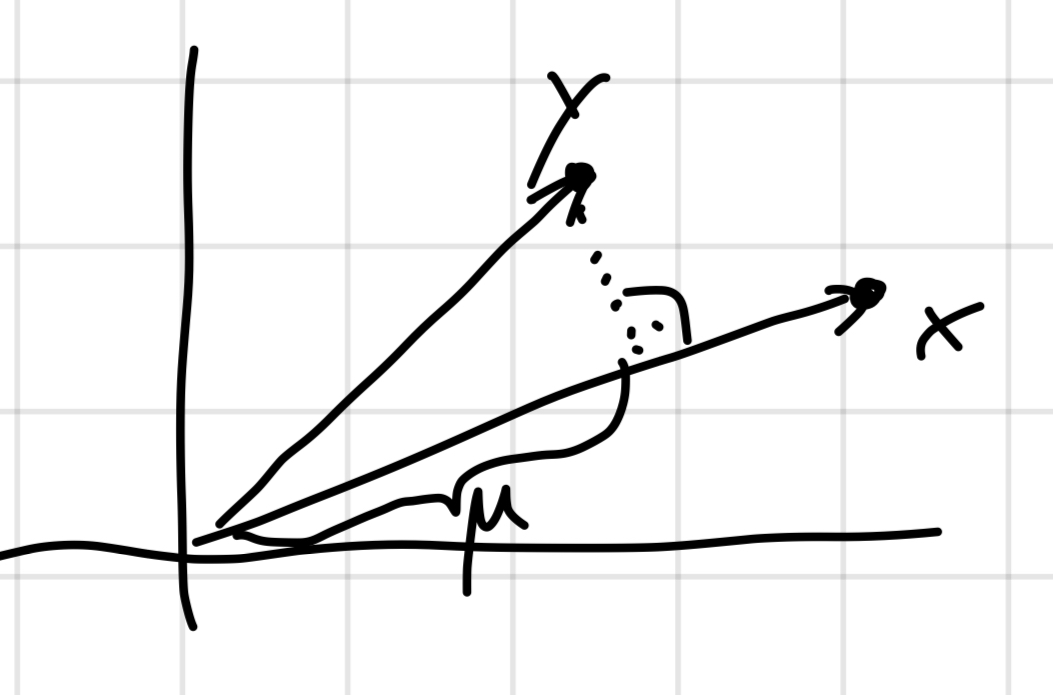
\includegraphics[width=0.5\textwidth]{Images/3.2.jpeg}
    \caption{}
\end{figure}

Das Skalarprodukt ist eine Abbildung $\mathbb{R}^2 \times \mathbb{R}^2 \rightarrow \mathbb{R}$ für welche folgende Rechenregeln gelten: \\
\subsubsection*{Lemma 3.3}
Für alle $x, x', y \in \mathbb{R}^2$ und $t \in \mathbb{R}$ gilt: \\
a) $\langle x + x', y \rangle = \langle x,y \rangle + \langle x',y \rangle$ \\
b) $\langle t \cdot x, y \rangle = t \cdot \langle x,y \rangle$ \\
c) $\langle x,y \rangle = \langle y,x \rangle$ \\
d) $\langle x,x \rangle > 0$ \\
e) $\langle x,x \rangle = 0 \Leftrightarrow x = (0,0)$ \\
Die Punkte a bis c ergeben zusammen Folgendes: \\
a') $\langle x, y+y' \rangle = \langle x,y \rangle + \langle x,y' \rangle$ \\
b') $\langle x, t \cdot y \rangle = t \cdot \langle x,y \rangle$ \\
\\
\subsubsection*{Definition 3.4}
Für $x \in \mathbb{R}^2$ heißt $\|x\| := \sqrt{\langle x,x \rangle}$ die \textit{Norm} von $x$. \\
Hinweis: Für Norm sagen wir auch Länge falls x durch einen Pfeil dargestellt wird. \\

\begin{figure}[h]
    \centering
    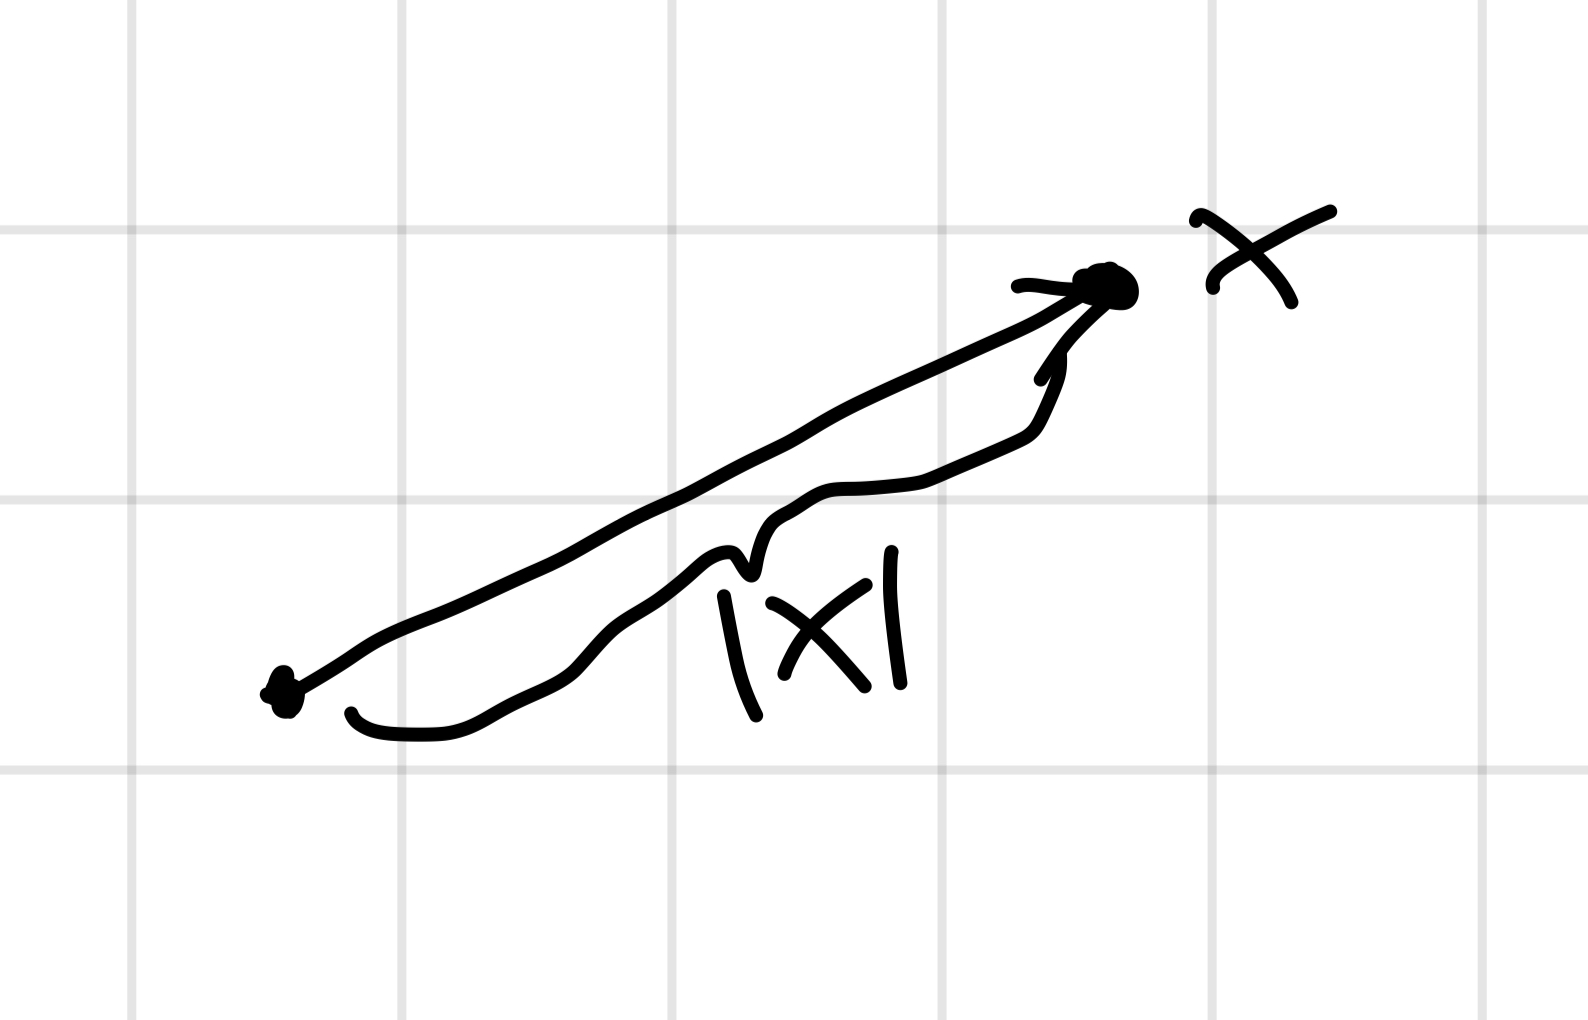
\includegraphics[width=0.5\textwidth]{Images/3.4.jpeg}
    \caption{}
\end{figure}

\subsubsection*{Bemerkung 3.5}
Wegen Lemma 3.3d ist $\sqrt{\langle x,x \rangle}$ immer wohldefiniert. \\
Für $x=(x_1, x_2)$ gilt $\|x\| = \sqrt{\langle x,x \rangle} = \sqrt{x_1 \cdot x_1 + x_2 \cdot x_2}$, was per Satz des Pythagoras wirklich die Länge von $x$ ist. \\

\begin{figure}[h]
    \centering
    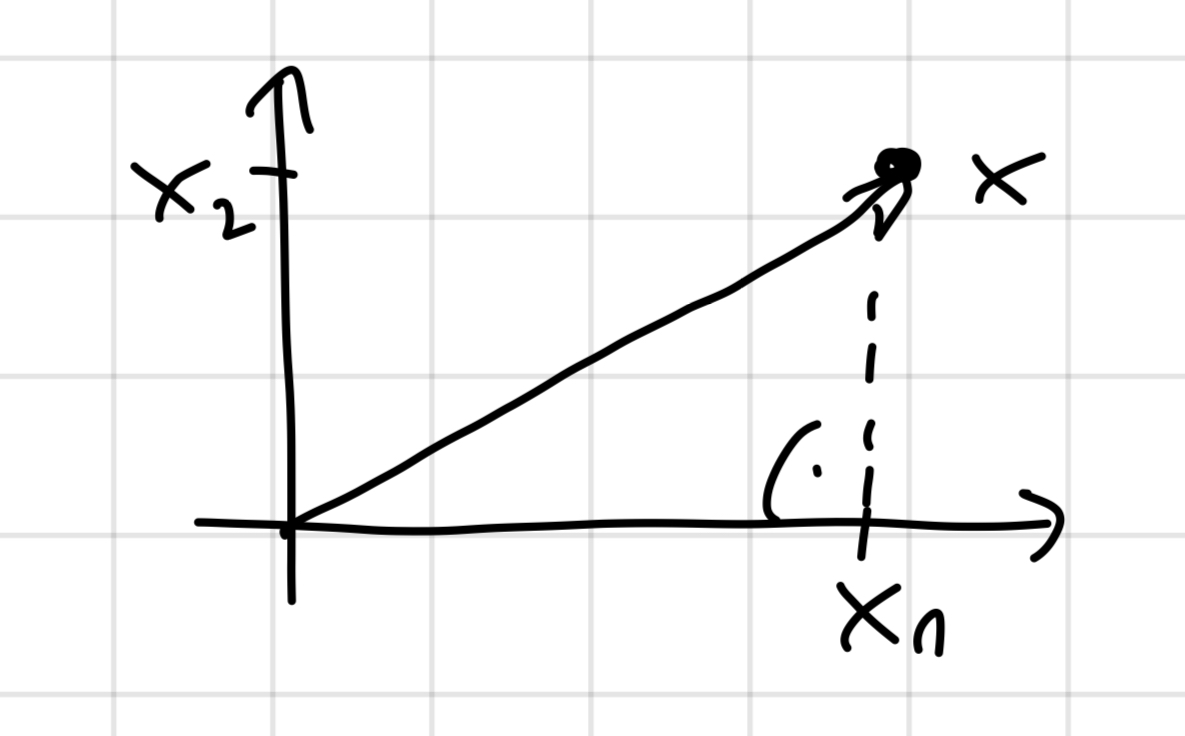
\includegraphics[width=0.5\textwidth]{Images/3.5.jpeg}
    \caption{}
\end{figure}

\subsubsection*{Satz 3.6 (Cauchy-Schwarz-Ungleichung)}
Für alle $x,y \in \mathbb{R}^2$ gilt: \\
\begin{center}
    $|\langle x,y \rangle| \leq \|x\| \cdot \|y\|$
\end{center}

\subsubsection*{Beweis}
Wir schreiben $x=(x_1, x_2)$ und $y=(y_1, y_2)$ und berechnen: \\
\begin{align*}
    (\|x\| \cdot \|y\|)^2 - (\langle x,y \rangle)^2 &= \|x\|^2 \cdot \|y\|^2 - \langle x,y \rangle^2 \\
    &= \langle x,x \rangle \cdot \langle y,y \rangle - \langle x,y \rangle^2 \\
    &= (x_1^2 + x_2^2) \cdot (y_1^2 + y_2^2) - (x_1 \cdot y_1 + x_2 \cdot y_2)^2 \\
    &= x_1^2 \cdot y_2^2 + x_2^2 \cdot y_1^2 + x_2^2 \cdot y_2^2 - (x_1^2 \cdot y_1^2 + 2 \cdot x_1 \cdot y_1 \cdot x_2 \cdot y_2 + x_2^2 \cdot y_2^2) \\
    &= x_2^2 \cdot y_1^2 + x_1^2 \cdot y_2^2 - 2 \cdot x_1 \cdot y_1 \cdot x_2 \cdot y_2 \\
    &= (x_2 \cdot y_1 - x_1 \cdot y_2)^2 \\
\end{align*}
d.h. $(\|x\| \cdot \|y\|)^2 \geq (\langle x,y \rangle)^2$. Da $\|x\| \geq 0$, $\|y\| \geq 0$ und $|\langle x,y \rangle| \geq 0$ ist, können wir die Wurzel ziehen und erhalten \\
\begin{center}
    $\|x\| \cdot \|y\| \geq |\langle x,y \rangle|$
\end{center}
$\square$ \\
Hinweise: Zeile 3: Definition des Skalarproduktes und in Zeile 4 kürzen wir. Beim Wurzelziehen im letzten Satz benutzen wir, das die Wurzelfunktion monoton steigend ist.
Was haben uns die ganzen Umformungen jetzt gebracht? Der letzte Ausdruck der Umformungen ist eine Quadratzahl und damit nicht negativ. \\

\subsubsection*{Lemma 3.7}
Für alle $x,y \in \mathbb{R}^2$ und $t \in \mathbb{R}$ gilt: \\
a) $\|x\| \geq 0$ \\
b) $\|x\| = 0 \Leftrightarrow x = (0,0)$ \\
c) $\|t \cdot x\| = |t| \cdot \|x\|$ \\
d) $\|x+y\| \leq \|x\| + \|y\|$ \\

\subsubsection*{Beweis}
a) ist klar aus der Definition $\|x\| = \sqrt{\langle x,x \rangle}$ da die Wurzelfunktion nie negative Werte produziert. \\
b) Es gilt \\
\begin{align*}
    \|x\| = 0 &\Leftrightarrow \sqrt{\langle x,x \rangle} = 0 \\
    &\Leftrightarrow \langle x,x \rangle = 0 \\
    % &\Leftrightarrow x_1^2 + x_2^2 = 0 \\
    % &\Leftrightarrow x_1 = 0 \text{ und } x_2 = 0 \\
    &\Leftrightarrow x = (0,0)
\end{align*}
Hinweis: im letzten Schritt benutzen wir das Lemma 3.3e. \\
c) Es gilt \\
\begin{align*}
    \|t \cdot x\| &= \sqrt{\langle t \cdot x, t \cdot x \rangle} \\
    &= \sqrt{t^2 \cdot \langle x,x \rangle} \\
    &= \sqrt{t^2} \cdot \sqrt{\langle x,x \rangle} \\
    &= |t| \cdot \|x\|
\end{align*}
d) Es gilt \\
\begin{align*}
    \|x+y\|^2 &= \langle x+y, x+y \rangle \\
    &= \langle x,x \rangle + \langle x,y \rangle + \langle y,x \rangle + \langle y,y \rangle \\
    &= \|x\|^2 + \overset{\text{$\leq 2 \|x\| \cdot \|y\|$ Cauchy-Schwarz}}{2 \cdot \langle x,y \rangle} + \|y\|^2 \\
    &= (\|x\| + \|y\|)^2
\end{align*}
und jetzt auf beiden Seiten die Wurzel ziehen. $\square$ \\
\\
\subsubsection*{Bemerkung 3.8}
Die Eigenschaft im Lemma 3.7d) heißt \textit{Dreiecksungleichung}: \\

\begin{figure}[h]
    \centering
    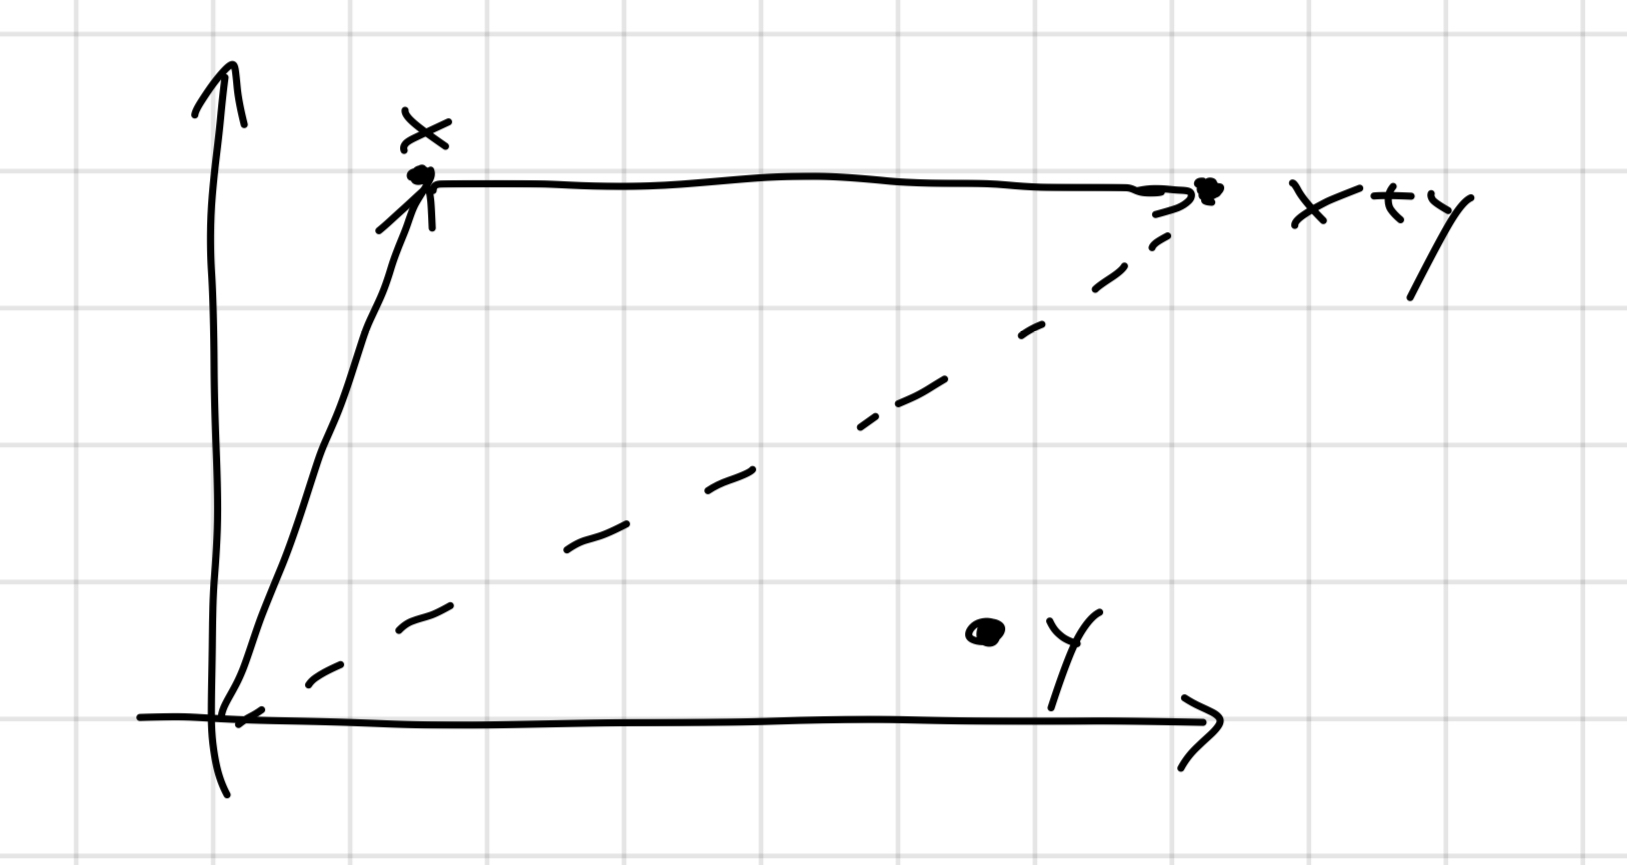
\includegraphics[width=0.5\textwidth]{Images/3.8.jpeg}
    \caption{}
\end{figure}

\subsubsection*{Definition 3.9}
Zu $x,y \in \mathbb{R}^2$ heißt \\
\begin{center}
    $d(x,y) := \|x-y\|$
\end{center}
der \textit{Abstand} von $x$ und $y$. \\

\subsubsection*{Lemma 3.10}
Für alle $x,y,z \in \mathbb{R}^2$ gilt: \\
a) $d(x,y) \geq 0$ \\
b) $d(x,y) = 0 \Leftrightarrow x = y$ \\
c) $d(x,y) = d(y,x)$ \\
d) $d(x,y) \leq d(x,z) + d(z,y)$ \\
Hinweis: Punkt d) ist die Dreiecksungleichung. \\
Der Beweis erfolgt per Nachrechnen unter unter Ausnutzung von Lemma 3.7. \\
\newpage
\date{Donnerstag, 30.11.23} \footnote{vgl. S. ? aus Baer.}
\subsection{Geraden und Dreiecke}
\subsubsection*{Definition 3.11}
Eine Gerade in der Ebene ist eine Menge der Form \\
\begin{center}
    $G_{a,v} := \{a + t \cdot v: t \in \mathbb{R}\}$ \\
\end{center}
wobei $a \in \mathbb{R}^2$ \textit{Aufpunkt} und $v \in \mathbb{R}^2\backslash\{0\}$ \textit{Richtungsvektor} der Gerade heißt. \\
\begin{figure}[h]
    \centering
    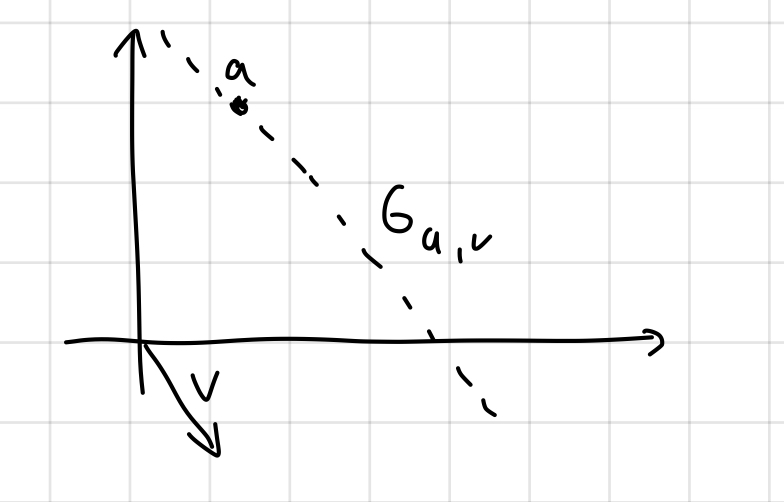
\includegraphics[width=0.5\textwidth]{Images/3.11.jpeg}
    \caption{}
\end{figure}

\subsubsection*{Anmerkung 3.12}
Wäre $v=(0,0)$ zugelassen, so wäre in diesem Fall $G_{a,v} = \{a\}$. Das ist aber anschaulich keine Gerade. \\

\subsubsection*{Lemma 3.13}
Es sei $G_{a,v}$ eine Gerade und $p \in G_{a,v}$. Dann gilt $G_{a,v} = G_{p,v}$. \\
\begin{figure}[h]
    \centering
    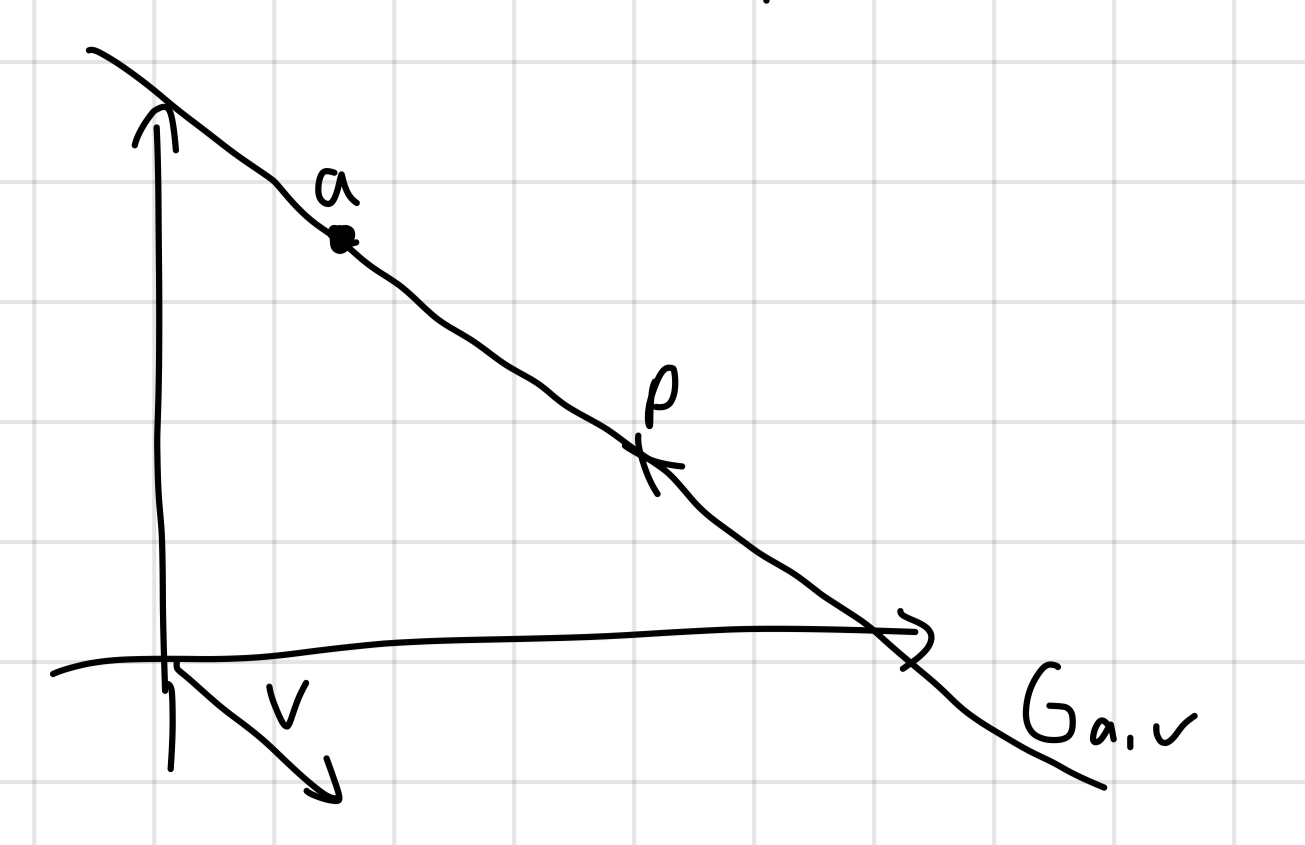
\includegraphics[width=0.5\textwidth]{Images/3.13.jpeg}
    \caption{}
\end{figure}

\subsubsection*{Beweis}
Wegen $p \in G_{a,v}$ gibt es ein $t \in \mathbb{R}$ mit $p = a + t \cdot v.^{(*)}$
\\
\underline{\textit{$G_{a,v} \supset G_{p,v}$}}: \\
Sei $q \in G_{p,v}$, d.h. es gibt ein $t_1 \in \mathbb{R}$ mit $q = p + t_1 \cdot v$. \\
Wir setzen (*) ein und erhalten \\
\begin{align*}
    q &= p + t_1 \cdot v \\
    &= (a + t_0 \cdot v) + t_1 \cdot v \\
    &= a + (t_0 + t_1) \cdot v
\end{align*}
d.h. $q \in G_{a,v}$. \\
\\
\underline{\textit{$G_{a,v} \subset G_{p,v}$}}: \\
Sei $x \in G_{a,v}$, d.h. es gibt ein $t_1 \in \mathbb{R}$ mit $x = a + t_1 \cdot v$. \\
Aus (*) folgt $a=p-t_0 \cdot v^{(**)}$ und damit \\
\begin{align*}
    x &= a + t_1 \cdot v \\
    &= p - t_0 \cdot v + t_1 \cdot v \\
    &= p + (t_1 - t_0) \cdot v
\end{align*}
d.h. $x \in G_{p,v}$. \\
$\square$ \\
\\
Hinweis: (**) wurde in Zeile 2 benutzt. \\
\\
\subsubsection*{Lemma 3.14}
Es sei $G \in \mathbb{R}^2$ eine Gerade. Sind $a,b \in G$ mit $a \neq b$, so ist \\
\begin{center}
    $G = G_{a,b-a}$  \\
\end{center}
Hinweis: 2 Punkte legen eine Gerade also eindeutig fest. \\
\\
\subsubsection*{Beweis}
$G$ ist eine Gerade, d.h. es gibt $p \in \mathbb{R}^2$ und $v \in \mathbb{R}^2\backslash\{0\}$ mit $G = G_{p,v}$. 
Wegen Lemma 3.13 gilt $G_{a,v} = G_{p,v}$. Wegen $b \in G = G_{a,v}$ gibt es ein $t_0 \in \mathbb{R}$ mit $b = a + t_0 \cdot v$. 
Wegen $b \neq a$ ist $t_0 \neq 0$. Wir zeigen jetzt, dass $G_{a,v} = G_{a,b-a}$: \\
\underline{\textit{$G_{a,v} \subset G_{a,b-a}$}}: \\
Zu jedem $x \in G_{a,v}$ gibt es ein $t_1 \in \mathbb{R}$ mit $x = a + t_1 \cdot v$.
Jetzt gilt: \\
\begin{align*}
    x &= a + t_1 \cdot v \\
    &= a + t_1 \cdot \frac{1}{t_0} \cdot (b-a) \\
\end{align*}
d.h. $x \in G_{a,b-a}$. \\
Hinweis: wir haben im Beweis genutzt, dass $b=a+t_0 \cdot v$ und $t_0 \neq 0$ und daraus folgt $v = \frac{1}{t_0} \cdot (b-a)$. \\
\\
\underline{\textit{$G_{a, b-a} \subset G_{a,v}$}}: \\
Für $y \in G_{a,b-a}$ existiert ein $t_2 \in \mathbb{R}$ mit $y = a + t_2 \cdot (b-a)$. \\
Dann gilt: \\
\begin{align*}
    y &= a + t_2 \cdot (b-a) \\
    &= a + t_2 \cdot t_0 \cdot v \\
\end{align*}
d.h. $y \in G_{a,v}$. \\
Hinweis: wir haben im Beweis genutzt, dass $b=a+t_0 \cdot v$ und daraus folgt $b-a = t_0 \cdot v$. \\
$\square$ \\
\\
\subsubsection*{Lemma 3.15 (Mittelpunktslemma)}
Sei $G \subset \mathbb{R}^2$ eine Gerade und $a,b \in G$ mit $a \neq b$. Dann existiert genau ein Punkt $c \in G$ mit $d(a,c) = d(b,c)$.
Für diesen Punkt $c$ gilt ferner: \\
\begin{center}
    $c = \frac{1}{2} \cdot (a+b)$
    und 
    $d(a,c) = \frac{1}{2} \cdot d(a,b) = d(b,c)$
\end{center}
Hinweis: in diesem Lemma sind 2 Aussagen versteckt: \\
1. Es gibt einen Punkt c, der von a und b den gleichen Abstand hat. \\
2. Dieser Punkt ist eindeutig definiert. Für diesen Punkt gilt, dass wir ihn als Mittelpunkt ausrechnen können. \\
Das kann man mit der Aussage verbinden, dass der kürzeste Weg zwischen 2 Punkten eine Gerade ist, da wenn ich die halbe Strecke laufe und auf dem Mittelpunkt lande, dann bin ich auf der Geraden. \\
\\
\subsubsection*{Beweis}
Nach Lemma 3.14 gilt, dass $G = G_{a,b-a}$ ist. Sei $q = a+t_0 \cdot (b-a) \in G$ für ein $t_0 \in \mathbb{R}$.
Dann gilt: \\
\begin{align*}
    d(a,q) &= \|a-q\| \\
    &= \|a-(a+t_0 \cdot (b-a))\| \\
    &= \|-t_0 \cdot (b-a)\| \\
    &= |-t_0| \cdot \|b-a\| \\
    &= |t_0| \cdot \|b-a\| \\
\end{align*}
und ebenso \\
\begin{align*}
    d(b,q) &= \|b-q\| \\
    &= \|b-(a+t_0 \cdot (b-a))\| \\
    &= \|b-a\underbrace{-t_0 \cdot (b+t_0 \cdot a)}_{=t_0(-b+a)}\| \\
    &= \|(1-t_0) \cdot (b-a)\| \\
    &= |1-t_0| \cdot \|b-a\| \\
\end{align*}
Damit gilt dann: \\
\begin{align*}
    d(a,q) = d(b,q) &\Leftrightarrow |t_0| \cdot \|b-a\| = |1-t_0| \cdot \|b-a\| \\
    &\Leftrightarrow |t_0| = |1-t_0| \\
    &\Leftrightarrow t_0^2 = (1-t_0)^2 \\
    &\Leftrightarrow t_0^2 = 1 - 2 \cdot t_0 + t_0^2 \\
    &\Leftrightarrow t_0 = \frac{1}{2} \\
\end{align*}
Damit ist $c = a + \frac{1}{2} \cdot (b-a) = \frac{1}{2} \cdot (a+b)$ der einzige Punkt auf $G$ der von $a$ und $b$ den gleichen Abstand hat. 
Für diesen Abstand gilt $d(a,c) = \frac{1}{2} \cdot \|b-a\| = d(b,c)$. \\
$\square$ \\
Hinweis: in Zeile 2 haben wir benutzt, dass $\|b-a\| \neq 0$ ist. 

\subsubsection*{Definition 3.16}
Ein Dreieck ist ein Tripel $(a,b,c)$ von Punkten $a,b,c \in \mathbb{R}^2$. Das Dreieck $(a,b,c)$ heißt \textit{entartet}, falls die Punkte $a,b,c$ auf einer Geraden liegen. \\
\\
\subsubsection*{Definition 3.17}
Eine Seitenhalbierende in einem nicht entarteten Dreieck ist eine Gerade durch eine der Ecken des Dreiecks sowie den Mittelpunkt der anderen beiden Ecken. \\
Die 3 Seitenhalbierenden sind: \\
\begin{center}
    $G_a,\frac{1}{2}(b+c)-a$ \\
    $G_b,\frac{1}{2}(a+c)-b$ \\
    $G_c,\frac{1}{2}(a+b)-c$ \\
\end{center}

\subsubsection*{Satz 3.18}
In jedem nicht-entarteten Dreieck schneiden sich die 3 Seitenhalbierenden im Punkt $\frac{1}{3}(a+b+c)$. \\
\begin{figure}[h]
    \centering
    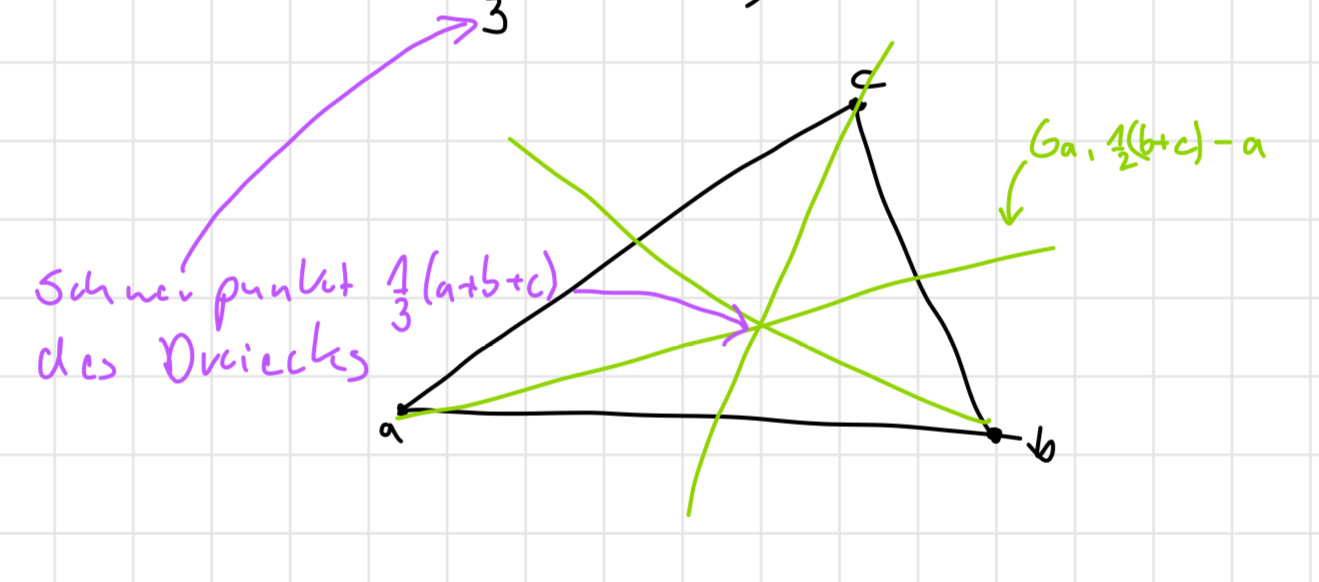
\includegraphics[width=0.5\textwidth]{Images/3.18.jpeg}
    \caption{}
\end{figure}

\subsubsection*{Beweis}
Wir zeigen, dass $\frac{1}{3}(a+b+c)$ auf allen Seitenhalbierenden liegt. \\
Für \\
\begin{center}
    $G_a, \frac{1}{2}(b+c)-a = \{a+t \cdot (\frac{1}{2}(b+c)-a): t \in \mathbb{R}\}$ \\
\end{center}
wählen wir $t = \frac{2}{3}$ und erhalten \\
\begin{align*}
    a + \frac{2}{3} \cdot (\frac{1}{2}(b+c)-a) &= a + \frac{1}{3}(b+c) - \frac{2}{3}a \\
    &= \frac{1}{3}(a+b+c)\\
\end{align*}
Analog verfährt man mit den beiden anderen Seitenhalbierenden. \\
$\square$ \\
\\
\subsubsection*{Anmerkung 3.19}
Der Schnittpunkt teilt die Seitenhalbierenden im Verhältnis $2:1$. \\
\begin{figure}[h]
    \centering
    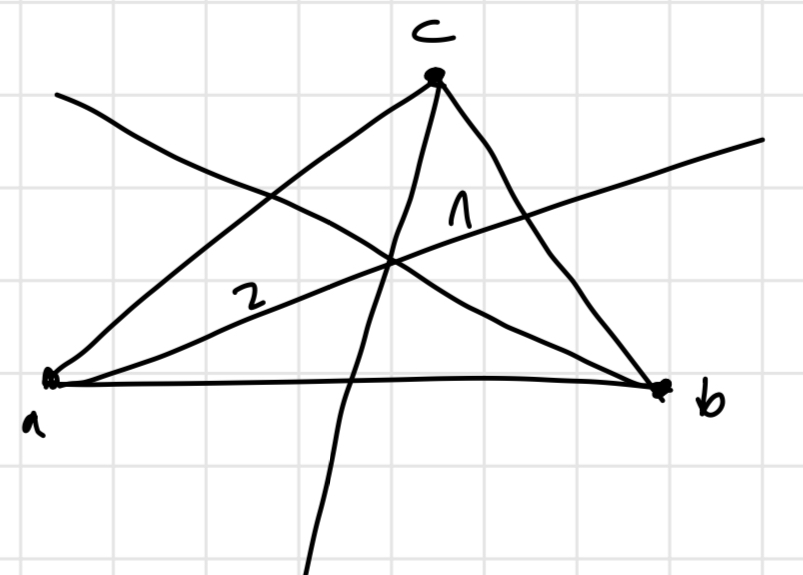
\includegraphics[width=0.5\textwidth]{Images/3.19.jpeg}
    \caption{}
\end{figure}

\newpage
\date{Mittwoch, 06.12.23} \footnote[1]{Die Inhalte dieser Vorlesung beziehen sich ungefähr auf Seite ? aus Baer.}
\subsection{Winkel}
Sind $x,y \in \mathbb{R}^2\backslash\{0\}$, so gilt \\
\begin{center}
    $\left| \frac{\langle x,y \rangle}{\|x\| \cdot \|y\|} \right| = \frac{|\langle x,y \rangle|}{\|x\| \cdot \|y\|} \leq \frac{\|x\| \cdot \|y\|}{\|x\| \cdot \|y\|} = 1$
\end{center}
d.h. $\frac{\langle x,y \rangle}{\|x\| \cdot \|y\|} \in [-1,1]$. \\
Wir erinnern uns an die Kosinusfunktion $\cos: [0,\pi] \rightarrow [-1,1]$, welche mit diesem Definitionsbereich und Zielbereich bijektiv ist. \\
\begin{figure}[h]
    \centering
    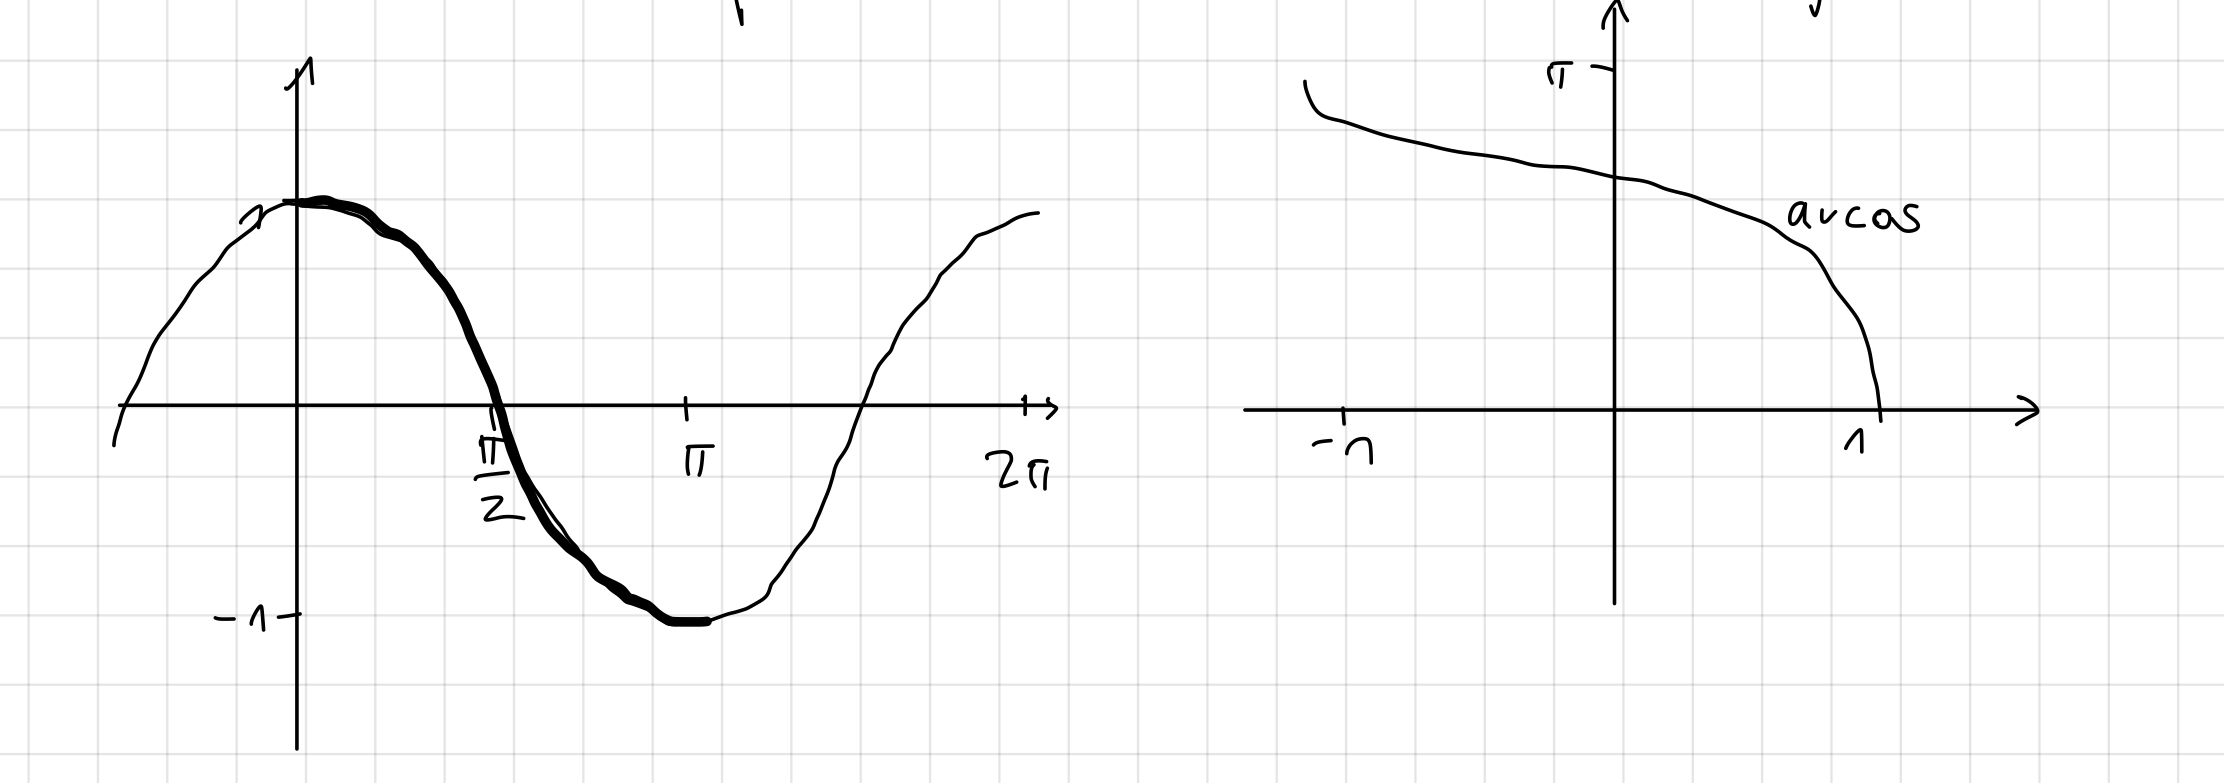
\includegraphics[width=0.5\textwidth]{Images/3.3.jpeg}
    \caption{}
\end{figure}
Sie hat also eine Umkehrfunktion $\arccos: [-1,1] \rightarrow [0,\pi]$. \\
\\
\subsubsection*{Definition 3.20}
Für $x,y \in \mathbb{R}^2\backslash\{0\}$ heißt die Zahl \\
\begin{center}
    $\measuredangle (x,y) := \arccos \left( \frac{\langle x,y \rangle}{\|x\| \cdot \|y\|} \right)$
\end{center}
der \textit{Innenwinkel} von $x$ und $y$ (nie mehr als 180 Grad). \\
\begin{figure}[h]
    \centering
    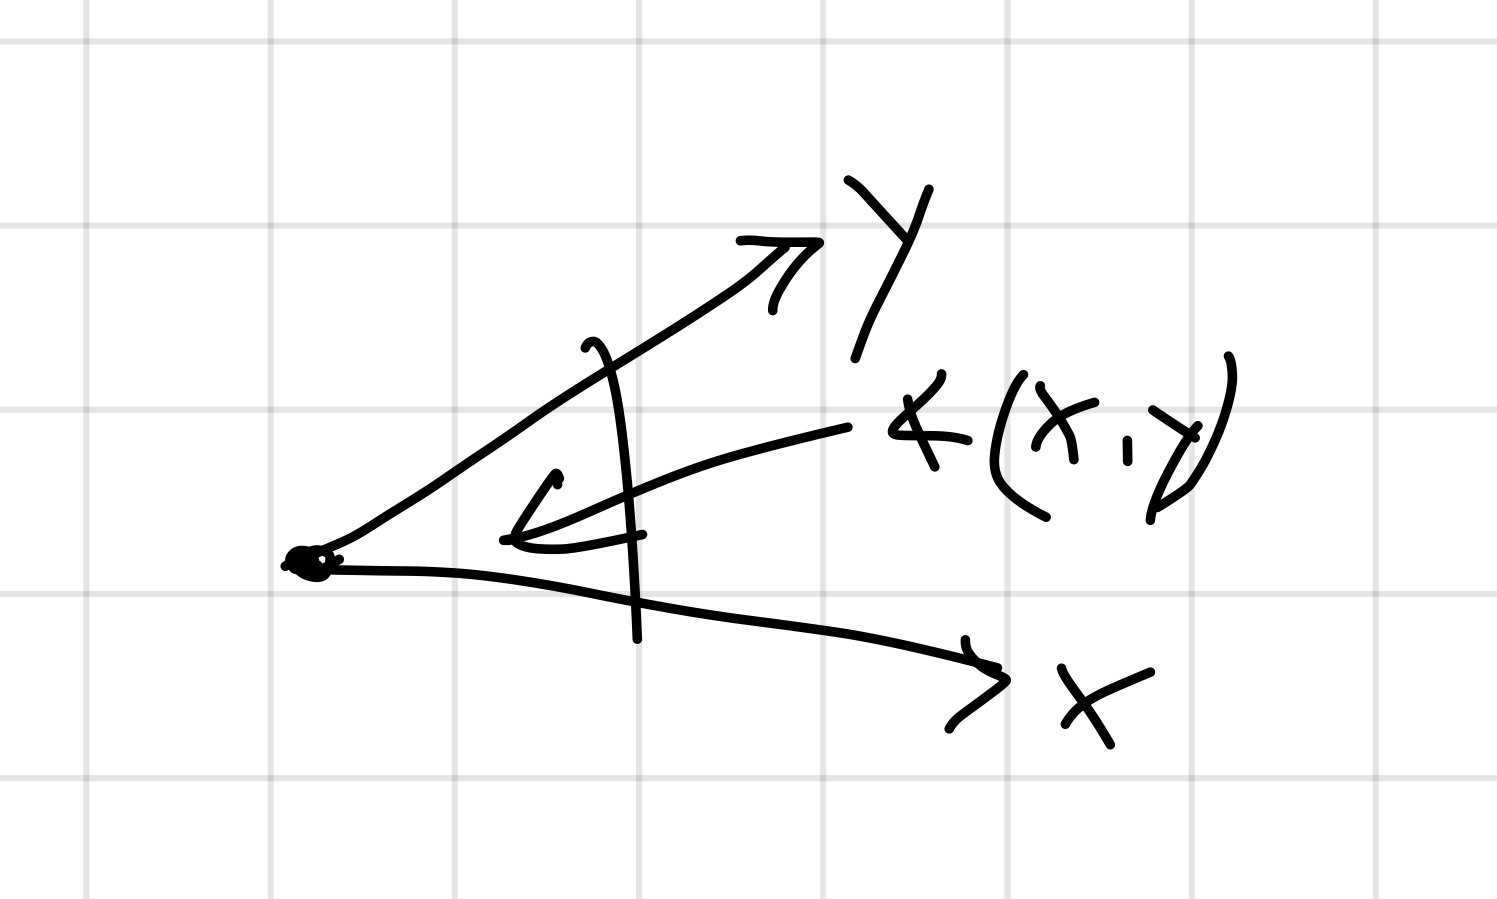
\includegraphics[width=0.5\textwidth]{Images/3.20.jpeg}
    \caption{}
\end{figure}
Obige Definition gibt den Winkel in Bogenmaß an, wo ein voller Kosinus dem Bogenmaß $\alpha \pi$ entspricht. \\
\\
\subsubsection*{Beispiele 3.21}
a) 
\begin{align*}
    \measuredangle (x,x) = \arccos \left( \frac{\langle x,x \rangle}{\|x\| \cdot \|x\|} \right) = \arccos \left( \frac{\|x\|^2}{\|x\| \cdot \|x\|} \right) = \arccos(1) = 0 \\
\end{align*}
b) 
\begin{align*}
    \measuredangle (x,-x) &= \arccos \left( \frac{\langle x,-x \rangle}{\|x\| \cdot \|-x\|} \right)\\
    &= \arccos \left( \frac{-\langle x,x \rangle}{\|x\| \cdot \|x\|} \right) \\
    &= \arccos(-1) \\
    &= \pi \triangleq 180^\circ \\
\end{align*}
\begin{figure}[h]
    \centering
    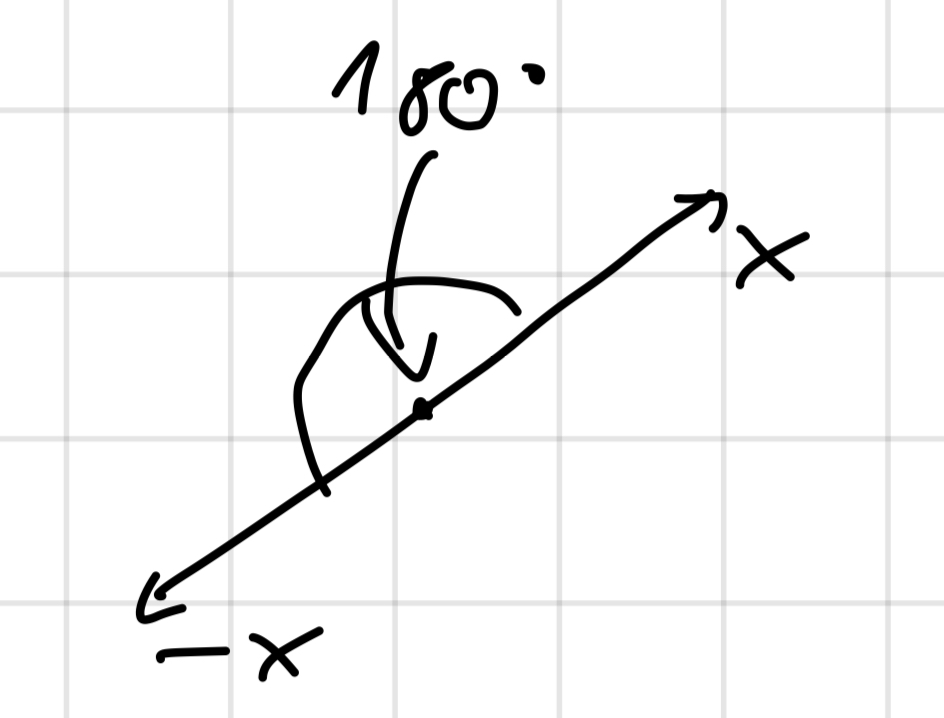
\includegraphics[width=0.5\textwidth]{Images/3.21b.jpeg}
    \caption{}
\end{figure}
c) 
Ist $\langle x,y \rangle = 0$, so gilt $\measuredangle (x,y) = \arccos \left( \frac{\langle x,y \rangle}{\|x\| \cdot \|y\|} \right) = \arccos(0) = \frac{\pi}{2} \triangleq 90^\circ$. \\
\begin{figure}[h]
    \centering
    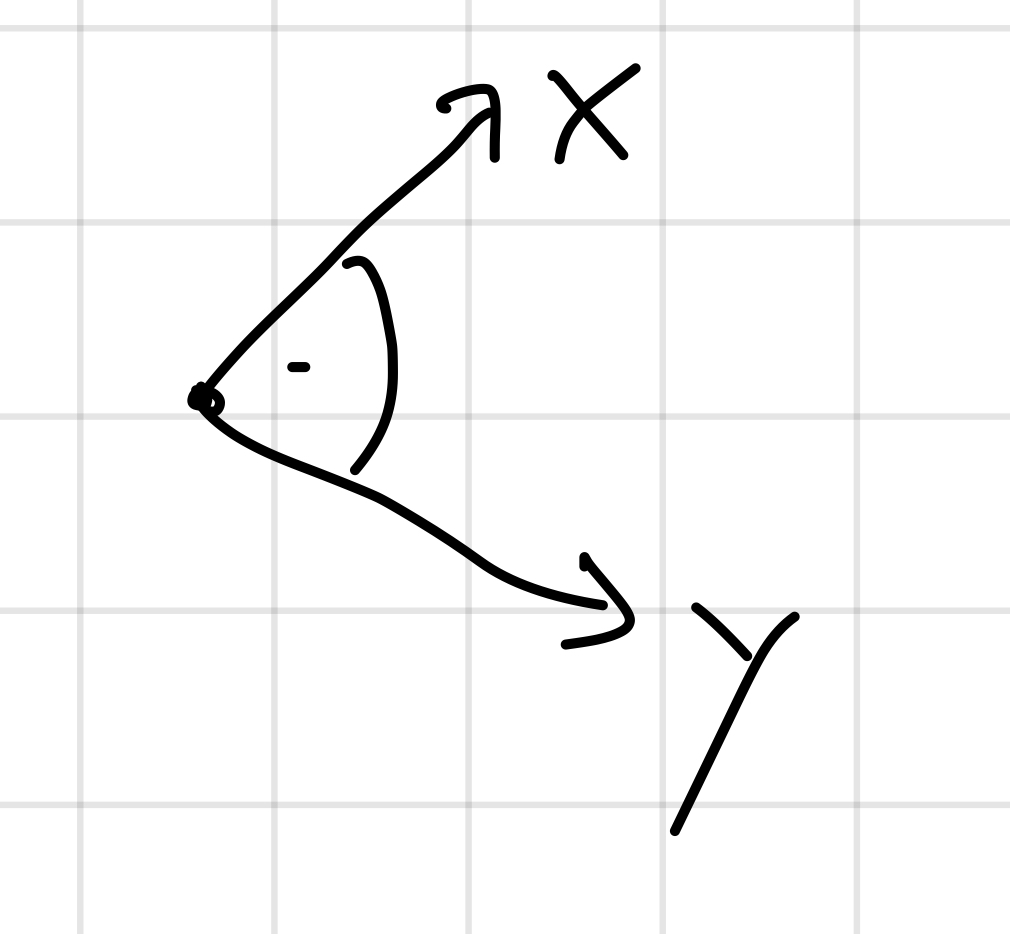
\includegraphics[width=0.5\textwidth]{Images/3.21c.jpeg}
    \caption{}
\end{figure}
\\
\subsubsection*{Definition 3.22}
Falls $\langle x,y \rangle = 0$, so heißen $x$ und $y$ \textit{orthogonal} zueinander, d.h. sie stehen senkrecht aufeinander. \\
\\
\subsubsection*{Satz 3.23 (Kosinussatz)}
Sei $(a,b,c)$ ein nicht-entartetes Dreieck und sei $\alpha = \measuredangle (b,c)^2 = d(a,b)^2 + d(a,c)^2 - 2 \cdot d(a,b) \cdot d(a,c) \cdot \cos(\alpha)$. \\
\begin{figure}[h]
    \centering
    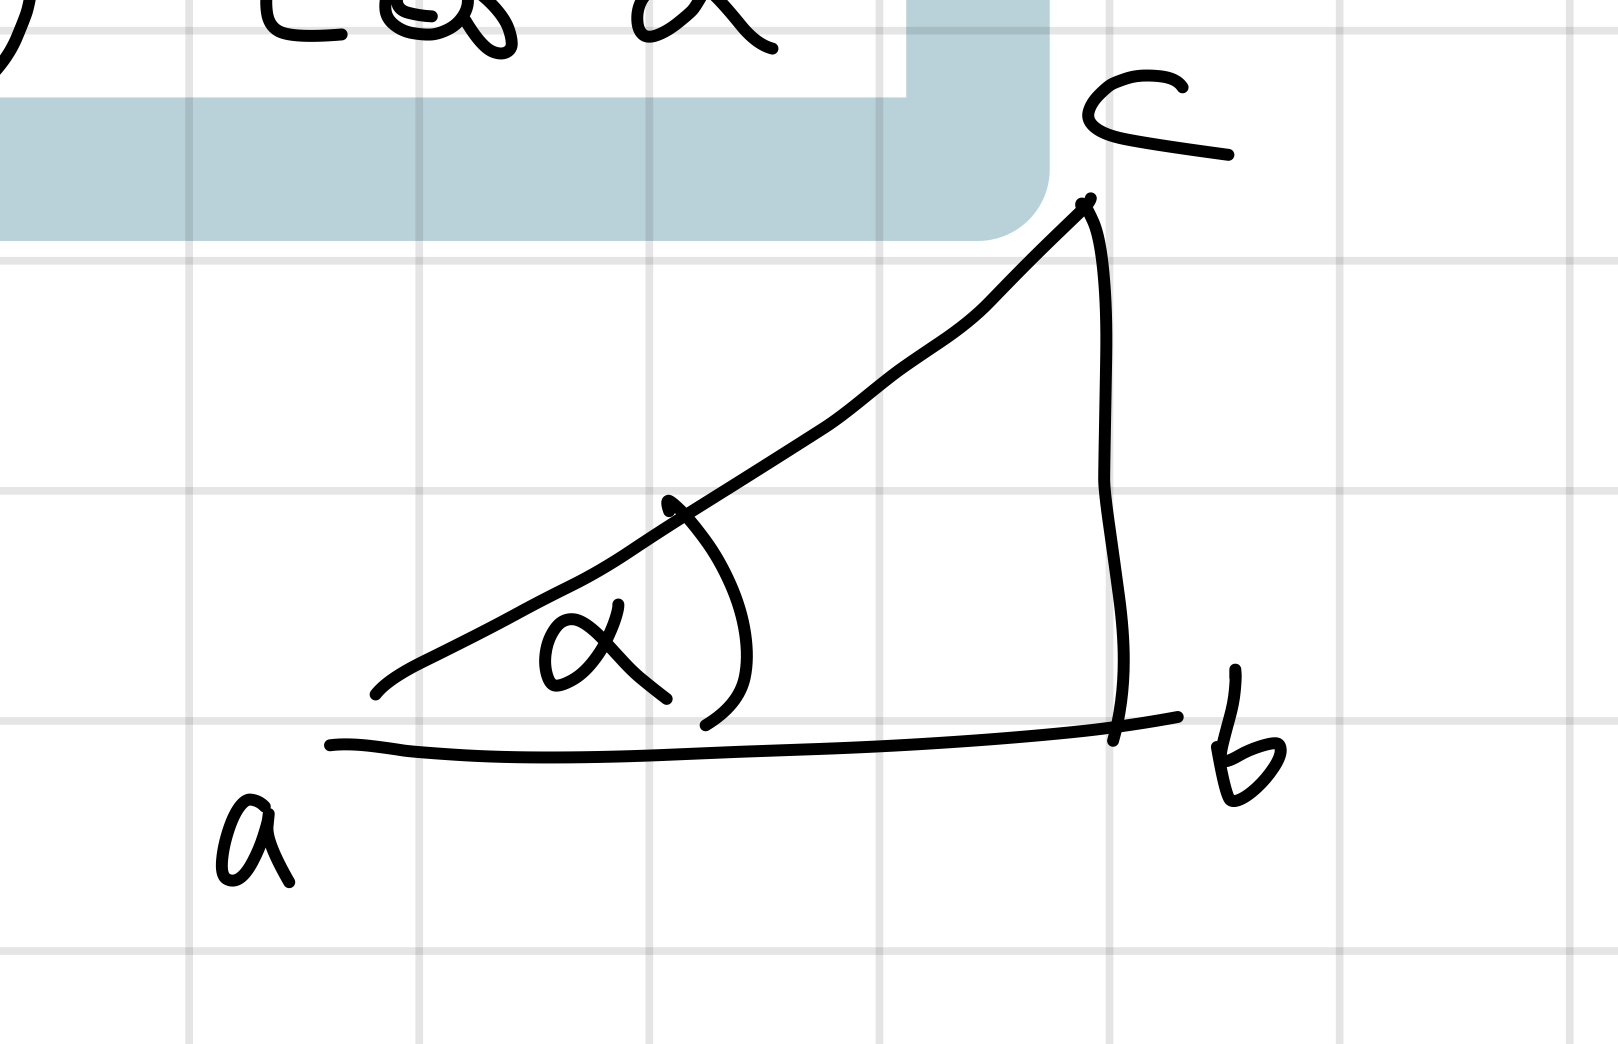
\includegraphics[width=0.5\textwidth]{Images/3.23.jpeg}
    \caption{}
\end{figure}  
\\
\subsubsection*{Beweis}
Wir weisen die umgestellte Gleichung \\
\begin{center}
    $d(b,c)^2 - d(a,b)^2 - d(a,c)^2 = -2 \cdot d(a,b) \cdot d(a,c) \cdot \cos(\alpha)$ \\
    % $\textcolor{red}{\langle \cancel{a-b},a-b \rangle \cdot \langle \cancel{a-c},a-c \rangle \cdot \frac{\langle b-a, c-a \rangle}{\cancel{\|b-a\|} \cdot \cancel{\|c-a\|}}}$ \\
\end{center}
nach: \\
\begin{align*}
    d(b,c)^2 - d(a,b)^2 - d(a,c)^2 &= \|c-b\|^2 - \|b-a\|^2 - \|c-a\|^2 \\
    &= \langle c-b,c-b \rangle - \langle b-a,b-a \rangle - \langle c-a,c-a \rangle \\
    &= \langle c,c \rangle - 2 \cdot \langle b,c \rangle + \langle b,b \rangle - (\langle b,b \rangle - 2 \cdot \langle a,b \rangle + \langle a,a \rangle) \\
    &- (\langle c,c \rangle - 2 \cdot \langle a,c \rangle + \langle a,a \rangle) \\
    &= -2 \cdot \langle b,c \rangle + 2 \cdot \langle a,b \rangle + 2 \cdot \langle a,c \rangle - 2 \cdot \langle a,a \rangle \\
    &= -2 \cdot (\langle b,c \rangle - \langle a,b \rangle - \langle a,c \rangle + \langle a,a \rangle) \\
    &= -2 \cdot \langle b-a,c-a \rangle \\
    &= -2 \cdot \langle b-a,c-a \rangle \cdot \frac{\langle b-a,c-a \rangle \cdot \langle a-c, a-c \rangle}{\|b-a\| \cdot \|c-a\|} \\
    &= -2 \cdot d(a,b) \cdot d(a,c) \cdot \cos(\alpha) \\
\end{align*}
$\square$ \\

\subsubsection*{Korollar 3.24}
Die Seitenlängen eines nicht entarteten Dreiecks legen die Innenwinkel eindeutig fest. \\
\\
\subsubsection*{Korollar 3.25 (Satz des Pythagoras)}
Ist $\alpha = \frac{\pi}{2}$, so gilt $d(a,b)^2 + d(a,c)^2 = d(b,c)^2$. \\
\\

\subsubsection*{Definition 3.26}
Für $\theta \in \mathbb{R}$ definieren wir die Drehmatrix \\
\begin{center}
    $R_\theta := \begin{pmatrix}
        \cos \theta & -\sin \theta \\
        \sin \theta & \cos \theta \\
    \end{pmatrix}$
\end{center}
Anschaulich ist $R_\theta \cdot v$ die Drehung von $v$ gegen den Uhrzeigersinn im Winkel $\theta$ (im Bogenmaß). \\

%Bild
\subsubsection*{Lemma 3.27}
a) Für $\theta := 0$ gilt $\varphi_{R_\theta} = \text{id}_{\mathbb{R}^2}$ \\
b) Für $\theta_1, \theta_2 \in \mathbb{R}$ gilt $R_{\theta_1} \cdot R_{\theta_2} = R_{\theta_1 + \theta_2}$ \\
c) Für $\theta \in \mathbb{R}$ gilt $R_\theta \cdot R_{-\theta} = \varepsilon_2 = R_{- \theta} \cdot R_\theta$ \\
Hinweise: in a ist $\varphi_{R_\theta}$ die induzierte Abbildung $\mathbb{R}^2 \rightarrow \mathbb{R}^2$ \\
In c ist $\varepsilon_2$ die Einheitsmatrix. \\
\\
\subsubsection*{Beweis}
Der Beweis erfolgt durch Nachrechnen (siehe Übung). \\


\subsubsection*{Lemma 3.28}
Für alle $v,w \in \mathbb{R}^2$ und alle Drehmatrizen $R_\theta$ gilt: \\
a) $\langle R_\theta \cdot v, R_\theta \cdot w \rangle = \langle v,w \rangle$ \\
b) $\|R_\theta \cdot v\| = \|v\|$ \\
c) $\measuredangle (R_\theta \cdot v, R_\theta \cdot w) = \measuredangle (v,w)$ \\
d) $\langle R_\theta \cdot v, v \rangle = \cos \theta \cdot \langle v,v \rangle$ \\
Interpretation von d: 
Wir haben:
\begin{align*}
    \measuredangle (R_\theta \cdot v, v) &= \arccos \left( \frac{\langle R_\theta \cdot v, v \rangle}{\|R_\theta \cdot v\| \cdot \|v\|} \right) \\
    &= \arccos \left( \frac{\cos \theta \langle v,v \rangle}{\|v\| \cdot \|v\|} \right) \\
    &= \arccos (\cos \theta) \\
    &= \theta \\
\end{align*}
Das heißt $R_\theta$ rotiert um den Winkel $\theta$. \\
\begin{figure}
    \centering
    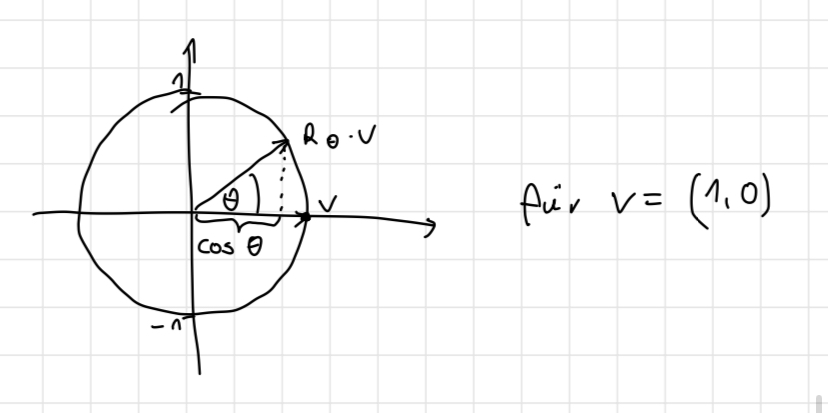
\includegraphics[width=0.5\textwidth]{Images/3.28.jpeg}
    \caption{}
\end{figure}

\subsubsection*{Beweis}
a) Für alle $v=(v_1, v_2), w=(w_1, w_2)$ und $\theta \in \mathbb{R}$ berechnen wir: \\
\begin{align*}
    \langle R_\theta \cdot v, R_\theta \cdot w \rangle &= \langle \begin{pmatrix}
        \cos \theta \cdot v_1 - \sin \theta \cdot v_2 \\
        \sin \theta \cdot v_1 + \cos \theta \cdot v_2 \\
    \end{pmatrix}, \begin{pmatrix}
        \cos \theta \cdot w_1 - \sin \theta \cdot w_2 \\
        \sin \theta \cdot w_1 + \cos \theta \cdot w_2 \\
    \end{pmatrix} \rangle \\
    &= (\cos \theta \cdot v_1 - \sin \theta \cdot v_2) \cdot (\cos \theta \cdot w_1 - \sin \theta \cdot w_2) \\
    &+ (\sin \theta \cdot v_1 + \cos \theta \cdot v_2) \cdot (\sin \theta \cdot w_1 + \cos \theta \cdot w_2) \\
    &= (\cos \theta)^2 \cdot v_1 w_1 - \sin \theta \cos \theta \cdot v_2 w_1 - \cos \theta \sin \theta \cdot v_1 w_2 + (\sin \theta)^2 \cdot v_2 w_2 \\
    &+ (\sin \theta)^2 \cdot v_1 w_1 + \cos \theta \sin \theta \cdot v_2 w_1 + \sin \theta \cos \theta \cdot v_1 w_2 + (\cos \theta)^2 \cdot v_2 w_2 \\
    &= v_1 w_1 + v_2 w_2 \\
    &= \langle \begin{pmatrix}
        v_1 \\
        v_2 \\
    \end{pmatrix}, \begin{pmatrix}
        w_1 \\
        w_2 \\
    \end{pmatrix} \rangle \\
    &= \langle v,w \rangle \\
\end{align*}
b) Folgt sofort aus a: \\
\begin{center}
    $\|R_\theta \cdot v\| = \sqrt{\langle R_\theta \cdot v, R_\theta \cdot v \rangle} = \sqrt{\langle v,v \rangle} = \|v\|$
\end{center}
c) Wir berechnen: \\
\begin{align*}
    \measuredangle (R_\theta \cdot v, R_\theta \cdot w) &= \arccos \left( \frac{\langle R_\theta \cdot v, R_\theta \cdot w \rangle}{\|R_\theta \cdot v\| \cdot \|R_\theta \cdot w\|} \right) \\
    &= \arccos \left( \frac{\langle v,w \rangle}{\|v\| \cdot \|w\|} \right) \\
    &= \arccos \left( \frac{\langle v,w \rangle}{\|v\| \cdot \|w\|} \right) \\
    &= \measuredangle (v,w) \\
\end{align*}
Ist a erfüllt, so sind auch b und c erfüllt. \\
d) Es gilt: \\
\begin{align*}
    \langle R_\theta \cdot v, v \rangle &= \langle \begin{pmatrix}
        \cos \theta \cdot v_1 - \sin \theta \cdot v_2 \\
        \sin \theta \cdot v_1 + \cos \theta \cdot v_2 \\
    \end{pmatrix}, \begin{pmatrix}
        v_1 \\
        v_2 \\
    \end{pmatrix} \rangle \\
    &= (\cos \theta \cdot v_1 - \sin \theta \cdot v_2) \cdot v_1 + (\sin \theta \cdot v_1 + \cos \theta \cdot v_2) \cdot v_2 \\
    &= \cos \theta \cdot v_1 \cdot v_1 + \cos \theta \cdot v_2 \cdot v_2 \\
    &= \cos \theta \cdot (v_1 v_1 + v_2 v_2) \\
    &= \cos \theta \cdot \langle v,v \rangle \\
\end{align*}

\date{Donnerstag, 07.12.23} \footnote{vgl. S. ? aus Baer.}
\subsection{Orthogonalität}
Wir definieren die Matrix \\
\begin{center}
    $\mathcal{J} := R_{\frac{\pi}{2}} = \begin{pmatrix}
        0 & -1 \\
        1 & 0 \\
    \end{pmatrix}$
\end{center}

\begin{figure}[h]
    \centering
    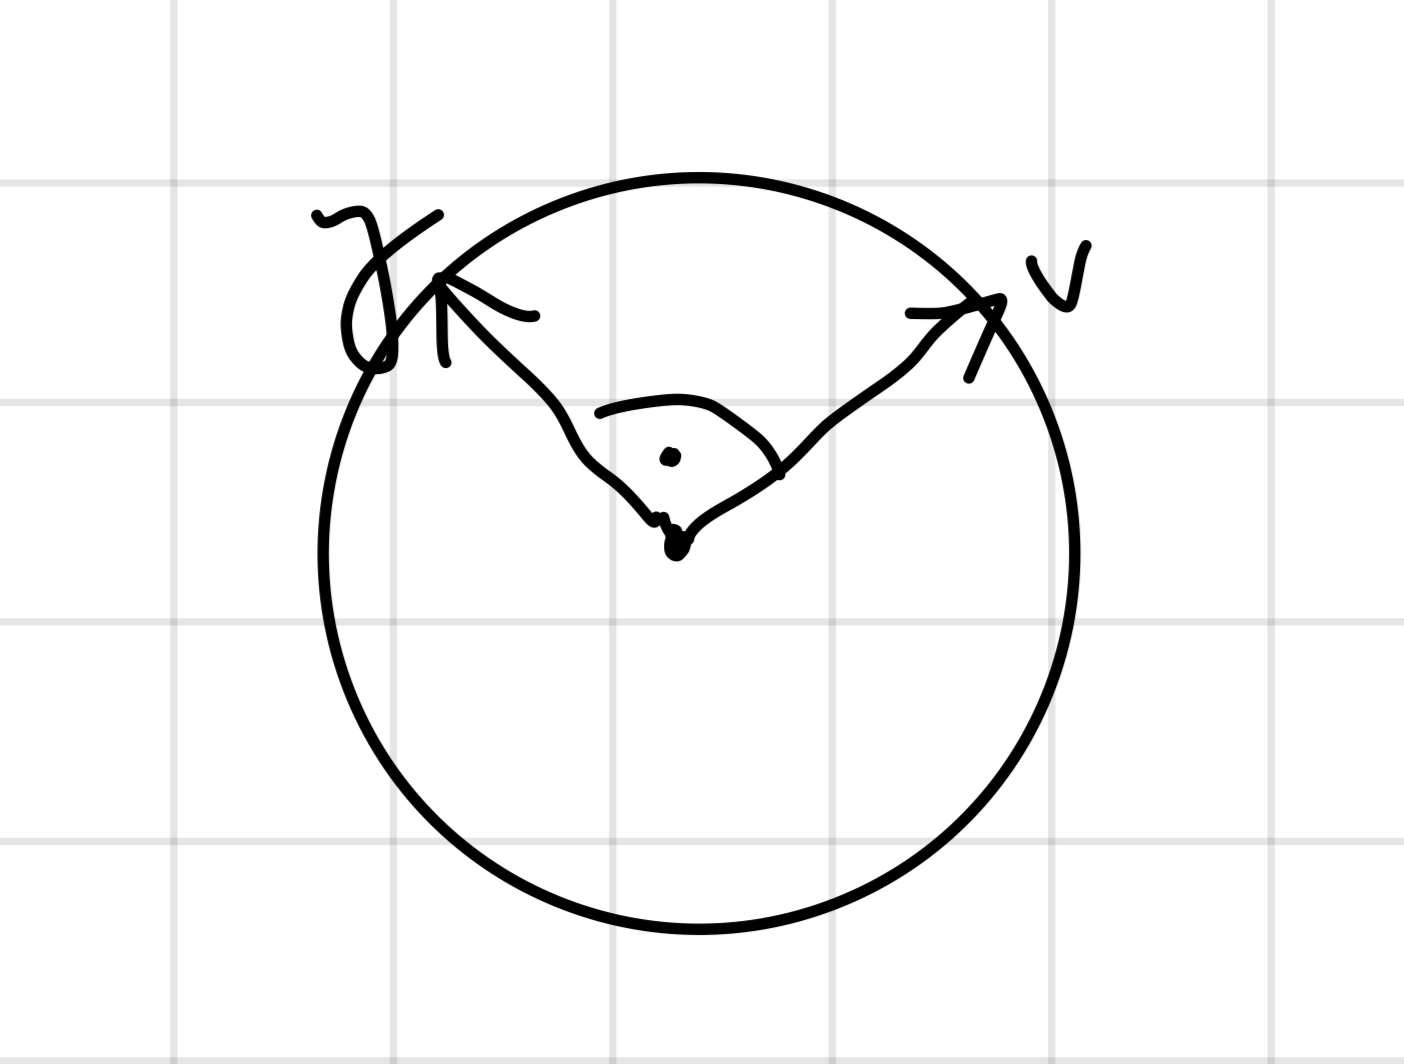
\includegraphics[width=0.5\textwidth]{Images/3.40.jpeg}
    \caption{$\mathcal{J}$ stellt die Drehung um 90 Grad gegen den Uhrzeigersinn dar.}
\end{figure}

\subsubsection*{Definition 3.29}
Für $\theta \in \mathbb{R}$ definieren wir die \textit{Spiegelungsmatrix} \\
\begin{center}
    $S_\theta := \begin{pmatrix}
        \cos 2\theta & \sin 2\theta \\
        \sin 2\theta & -\cos 2\theta \\
    \end{pmatrix}$
\end{center}
\begin{figure}[h]
    \centering
    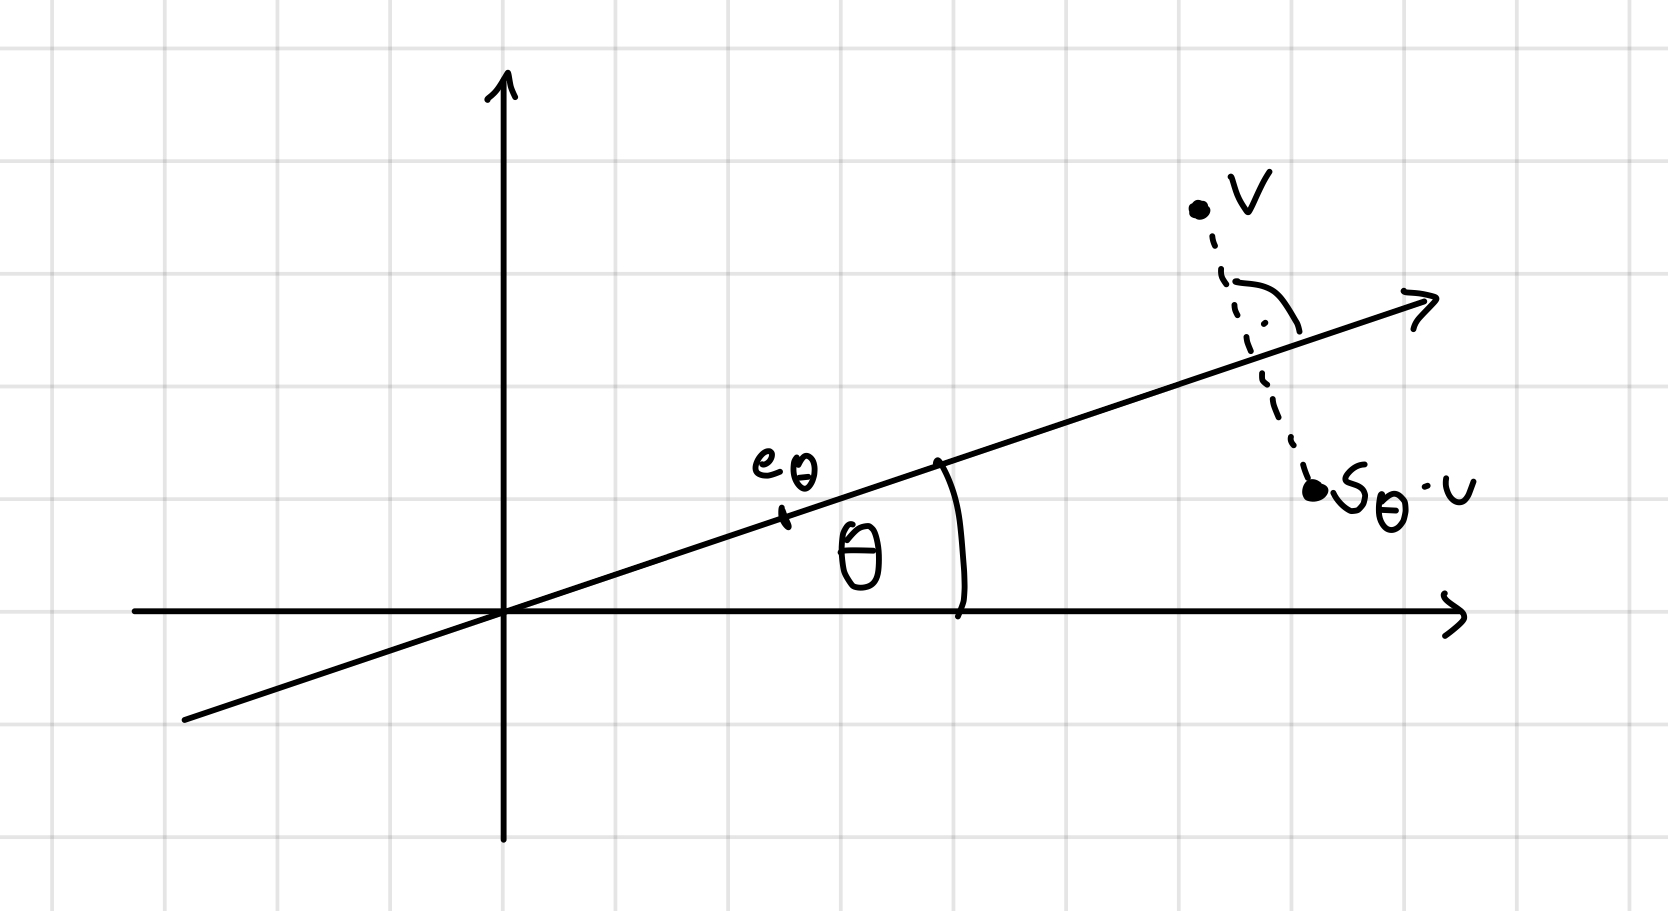
\includegraphics[width=0.5\textwidth]{Images/3.29.jpeg}
    \caption{Anschaulich ist $S_\theta \cdot v$ die Spiegelung von $v$ an der Geraden mit dem Winkel $\theta$ zur $x$-Achse.    }
\end{figure}

\subsubsection*{Lemma 3.30}
Sei $\theta \in \mathbb{R}$ und setze $e_\theta := \begin{pmatrix}
    \cos \theta \\
    \sin \theta \\
\end{pmatrix} \in \mathbb{R}^2$. Dann gilt: \\
a) $S_\theta \cdot e_\theta = e_\theta$ \\
b) $S_\theta \cdot (\mathcal{J} \cdot e_\theta) = -(\mathcal{J} \cdot e_\theta)$ \\
Die beiden Punkte zeigen die genaue Interpretation von $S_\theta$ als Spiegelung. \\
\\
\subsubsection*{Beweis}
a) Es gilt: \\
\begin{align*}
    S_\theta \cdot e_\theta &= \begin{pmatrix}
        \cos 2\theta \cdot \cos \theta + \sin 2\theta \cdot \sin \theta \\
        \sin 2\theta \cdot \cos \theta - \cos 2\theta \cdot \sin \theta \\ 
    \end{pmatrix} \\
    &= \begin{pmatrix}
        \cos \theta \\
        \sin \theta \\
    \end{pmatrix} \\
    &= e_\theta \\
\end{align*}
Hinweis: in der 2. Zeile haben wir die Additionstheoreme benutzt.
b) Analog zur selbstständigen Übung.
$\square$ \\
\\
\subsubsection*{Lemma 3.31}
Für alle $v,w \in \mathbb{R}^2$ und alle $\theta \in \mathbb{R}$ gilt: \\   
a) $\langle S_\theta \cdot v, S_\theta \cdot w \rangle = \langle v,w \rangle$ \\
b) $\|S_\theta \cdot v\| = \|v\|$ \\
c) $\measuredangle (S_\theta \cdot v, S_\theta \cdot w) = \measuredangle (v,w)$ \\
\\
\subsubsection*{Beweis}
Der Beweis ist komplett analog zu dem von Lemma 3.28. \\
\\
\subsubsection*{Lemma 3.32}
Für alle $\theta_1, \theta_2 \in \mathbb{R}$ gilt: \\
a) $S_{\theta_1} \cdot S_{\theta_2} = R_{2 (\theta_1 - \theta_2)}$ \\
b) $S_{\theta_1} \cdot R_{\theta_2} = S_{\theta_1 - \frac{\theta_2}{2}}$ \\
c) $R_{\theta_1} \cdot S_{\theta_2} = S_{\theta_2 + \frac{\theta_1}{2}}$ \\
Beweis per direktem Nachrechnen mit Hilfe der Additionstheoreme in den Übungen. \\
% \begin{figure}[h]
%     \centering
%     \includegraphics[width=0.5\textwidth]{Images/3.32.jpeg}
%     \caption{}
% \end{figure}

\subsubsection*{Satz 3.33}
Es sei $T$ eine $(2 \times 2)$-Matrix. Dann sind die folgenden beiden äquivalent zueinander: \\
a) Es gilt $\langle T \cdot v, T \cdot w \rangle = \langle v,w \rangle$ für alle $v,w \in \mathbb{R}^2$. \\
b) Es ist $T$ eine Rotations- oder Spiegelungsmatrix. \\
\\
\subsubsection*{Beweis}
a) $b \Rightarrow a$: \\
Die Implikation ist Lemma 3.28 a) bzw. Lemma 3.31 a). \\
Es gelte $\langle T \cdot v, T \cdot w \rangle = \langle v,w \rangle$ für alle $v,w \in \mathbb{R}^2$. \\
Dann gilt für $e_1 = (1,0) \in \mathbb{R}^2$: \\
\begin{align*}
    \|T \cdot e_1\| &= \sqrt{\langle T \cdot e_1, T \cdot e_1 \rangle} \\
    &= \sqrt{\langle e_1, e_1 \rangle} \\
    &= \|e_1\| \\
    &= 1 \\
\end{align*}
d.h. $T \cdot e_1 = (\cos \theta, \sin \theta)$ für ein $\theta \in \mathbb{R}$. \\
Analog sieht man $\|T \cdot e_2\| = 1$ für $e_2 = (0,1)$ und außerdem gilt $\langle T \cdot e_1, T \cdot e_2 \rangle = \langle e_1, e_2 \rangle = 0$, d.h. $T \cdot e_1$ steht senkrecht auf $T \cdot e_2$. 
Daher ist $T \cdot e_2 \pm (\sin \theta, \cos \theta)$. Im Falle $T \cdot e_2 = (-\sin \theta, \cos \theta)$ gilt: \\
\begin{align*}
    T = \begin{pmatrix}
        \cos \theta & -\sin \theta \\
        \sin \theta & \cos \theta \\
    \end{pmatrix}
\end{align*}
(Hinweis: die erste Spalte ist $T \cdot e_1$ und die 2. Spalte ist $T \cdot e_2$. Außerdem: wenn wir die i-te Spalte einer Matrix wissen wollen, dann multiplizieren wir die Matrix mit dem i-ten Einheitsvektor.)
und im Falle $T \cdot e_2 = (-\sin \theta, \cos \theta)$ gilt: \\
\begin{align*}
    T = \begin{pmatrix}
        \cos \theta & \sin \theta \\
        \sin \theta & -\cos \theta \\
    \end{pmatrix}
    = S_{\frac{\theta}{2}}
\end{align*}
$\square$ \\
% \begin{figure}[h]
%     \centering
%     \includegraphics[width=0.5\textwidth]{Images/3.33.jpeg}
%     \caption{}
% \end{figure}
\\
\subsubsection*{Definition 3.34}
Wir definieren $\mathcal{O}(2)$ als die Menge aller $(2 \times 2)$-Matrizen $T$ für die gilt: \\
\begin{center}
    $\langle T \cdot v, T \cdot w \rangle = \langle v,w \rangle$ für alle $v,w \in \mathbb{R}^2$ \\
\end{center}

\subsubsection*{Lemma 3.35}
a) Für alle $S, T \in \mathcal{O}(2)$ gilt $S \cdot T \in \mathcal{O}(2)$. \\
b) Für alle $R, S, T \in \mathcal{O}(2)$ gilt $R \cdot (S \cdot T) = (R \cdot S) \cdot T$. \\
c) Es ist $E \in \mathcal{O}(2)$ und für alle $T \in \mathcal{O}(2)$ gilt $T \cdot E_2 = T = E_2 \cdot T$. \\
d) Für alle $T \in \mathcal{O}(2)$ gibt es ein $S \in \mathcal{O}(2)$ mit $T \cdot S = E_2 = S \cdot T$. \\
Hinweis: das ist die Definition einer Gruppe in einem Spezialfall. \\
\\
\subsubsection*{Beweis}
a) Für alle $v,w \in \mathbb{R}^2$ gilt: \\
\begin{align*}
    \langle (S \cdot T) \cdot v, (S \cdot T) \cdot w \rangle &= \langle S (T \cdot v), S (T \cdot w) \rangle \\
    &= \langle T \cdot v, T \cdot w \rangle \\
    &= \langle v,w \rangle \\
\end{align*}
d.h. $S \cdot T \in \mathcal{O}(2)$. \\
b) Schema gezeigt in Lemma 2.36. \\
c) $E_2 \in \mathcal{O}(2)$ ist offensichtlich, da $E_2 \cdot v = v$ für alle $v \in \mathbb{R}^2$ und $T \cdot E_2 = T = E_2 \cdot T$ ist schon in Bemerkung 2.37 erwähnt worden. \\
d) Wir betrachten Satz 3.33. \\
\underline{Fall 1:} Wähle $S := R_{-\theta}$. 
\underline {Fall 2:} Wähle $S := S_\theta$. \\
$\square$ \\

\newpage
\subsection{Kongruenzabbildungen}
\subsubsection*{Definition 3.36}
Eine Abbildung $F: \mathbb{R}^2 \rightarrow \mathbb{R}^2$ der Form $F(x)=Ax+b$ mit $A \in \mathcal{O}(2)$ und $b \in \mathbb{R}^2$ heißt \textit{Kongruenzabbildung} oder auch \textit{euklidische Bewegung in der Ebene}. \\
Wir beweisen heute: \\
\subsubsection*{Satz 3.37}
Es sei $F: \mathbb{R}^2 \rightarrow \mathbb{R}^2$ eine Abbildung. Dann sind äquivalent: \\
a) $F$ ist eine euklidische Bewegung. \\
b) $F$ ist Abstandserhaltend, d.h. für alle $p,q \in \mathbb{R}^2$ gilt $d(F(p),F(q)) = d(p,q)$. \\
Was ist z.B. mit einer Drehung um den Winkel $\theta$ um einen Punkt $p$? \\
So eine Abbildung ist eine Verkettung der Verschiebung um $-p$, der Drehung um $\theta$ um den Koordinatenursprung und der anschließenden Rückverschiebung um $p$: \\
\begin{center}
    $x \mapsto R_\theta (x-p)+p = R_\theta \cdot x + (p-R_\theta \cdot p)$ \\
\end{center}
Also eine Kongruenzabbildung im Sinne der Definition 3.36. \\
\\
\subsubsection*{Beweis}
\textit{a) $\Rightarrow$ b)}: \\
Sei $F$ von der Form $F(x)=Ax+b$ mit $A \in \mathcal{O}(2)$ und $b \in \mathbb{R}^2$. Dann gilt für $x,y \in \mathbb{R}^2$: \\
\begin{align*}
    d(F(x),F(y)) &= \|F(x)-F(y)\| \\
    &= \|Ax+b-(Ay-b)\| \\
    &= \|Ax-Ay\| \\
    &= \|A(x-y)\|\\
    &= \|x-y\| \\
    &= d(x,y) \\
\end{align*}
Hinweise: \\
In Zeile 4 haben wir das Lemma 2.26 und Bemerkung 2.34 benutzt. \\
In Zeile 5 haben wir das Lemma 3.28 b) bzw. Lemma 3.31 b) benutzt. \\
\\
\textit{b) $\Rightarrow$ a)}: \\
Sei $F$ abstandserhaltend. Wir setzen $b = F(0)$ und $\varphi(x) := F(x) - b$ für $x \in \mathbb{R}^2$. Dann ist $\varphi(0) = F(0) - b = 0$ und wir zeigen gleich, dass $\varphi$ eine Matrixabbildung ist, deren Matrix in $\mathcal{O}(2)$ liegt. \\
\textit{Schritt 1}: \\
Wir zeigen $\langle \varphi(x), \varphi(y) \rangle = \langle x,y \rangle$ für alle $x,y \in \mathbb{R}^2$. Wir betrachten das Dreieck $(0,x,y)$. Die Abbildung $F$ bildet es auf $(b, F(x), F(y))$ ab und die Seitenlängen bleiben gleich! Translationen sind ebenso abstandserhaltend und deswegen hat dann das Dreieck $(0,\varphi(x),\varphi(y))$ ebenso die selben Seitenlängen wie das Dreieck $(0,x,y)$. \\
Wegen Korollar 3.24 sind also die Innenwinkel von $(0,\varphi(x),\varphi(y))$ und $(0,x,y)$ gleich, insbesondere also $\measuredangle (\varphi(x),\varphi(y)) = \measuredangle (x,y)$. Damit ergibt sich: \\
\begin{align*}
    \langle \varphi(x), \varphi(y) \rangle &= \cos (\measuredangle (\varphi(x),\varphi(y))) \cdot \|\varphi(x)\| \cdot \|\varphi(y)\| \\
    &= \cos (\measuredangle (x,y)) \cdot d(\varphi(x),0) \cdot d(\varphi(y),0) \\
    &= \cos (\measuredangle (x,y)) \cdot d(F(x),b) \cdot d(F(y),b) \\
    &= \cos (\measuredangle (x,y)) \cdot d(F(x), F(0)) \cdot d(F(y), F(0)) \\
    &= \cos (\measuredangle (x,y)) \cdot d(x,0) \cdot d(y,0) \\
    &= \cos (\measuredangle (x,y)) \cdot \|x\| \cdot \|y\| \\
    &= \langle x,y \rangle \\
\end{align*}
\textit{Schritt 2}: \\
Wir zeigen, dass $\varphi$ eine Matrixabbildung ist. \\
Es sei $e_1 = (1,0)$ und $e_2 = (0,1)$ und wir setzen $f(e_1) := \varphi(e_1)$ und $f(e_2) := \varphi(e_2)$. Für $i \in \{1,2\}$ gilt dann sowohl \\
\begin{center}
    $\|f_i\|^2 = \langle f_i, f_i \rangle = \langle \varphi(e_i), \varphi(e_i) \rangle = \langle e_i, e_i \rangle = \|e_i\|^2 = 1$ \\
\end{center}
als auch \\
\begin{center}
    $\langle f_i, f_j \rangle = \langle \varphi(e_i), \varphi(e_j) \rangle = \langle e_i, e_j \rangle = 0$ \\
\end{center}
Es sei nun $x \in \mathbb{R}^2$ und wir schreiben $x = (x_1, x_2)$. Wegen Aufgabe 4 des Blatts für die Übungen 7 können wir \\
\begin{center}
    $\varphi(x) \overset{\textcolor{red}{(*)}}{=} \alpha_1 f_1 + \alpha_2 f_2$
\end{center}
mit geeigneten Koeffizienten $\alpha_1, \alpha_2 \in \mathbb{R}$ schreiben. \\
Dann gilt einerseits:\\
\begin{align*}
    \langle \varphi(x), f_i \rangle &= \langle \varphi(x), \varphi(e_i) \rangle = \langle x, e_i \rangle = x_i \\
\end{align*}
und andererseits \\
\begin{align*}
    \langle \varphi(x), f_i \rangle &= \langle \alpha_1 f_1 + \alpha_2 f_2, f_i \rangle \\
    &= \alpha_1 \langle f_1, f_i \rangle + \alpha_2 \langle f_2, f_i \rangle \\
    &= \alpha_i \\
\end{align*}
für $i \in \{1,2\}$. \\
Wir folgern $x_1 \overset{\textcolor{darkgreen}{(*)}}{=} \alpha_1$ und $x_2 \overset{\textcolor{darkgreen}{(*)}}{=} \alpha_2$ und damit gilt, mit der Notation $f_1 \overset{\textcolor{darkgreen}{(*)}}{=} (\alpha_11, \alpha_21)$ und $f_2 \overset{\textcolor{darkgreen}{(*)}}{=} (\alpha_12, \alpha_22)$: \\
\begin{align*}
    \varphi(x) &\overset{\textcolor{red}{(*)}}{=} \alpha_1 f_1 + \alpha_2 f_2 \\
    & \overset{\textcolor{darkgreen}{(*)}}{=} x_1 \cdot \begin{pmatrix}
        \alpha_{11} \\
        \alpha_{21} \\
    \end{pmatrix} + x_2 \cdot \begin{pmatrix}
        \alpha_{12} \\
        \alpha_{22} \\
    \end{pmatrix} \\
    &= \begin{pmatrix}
        x_1 \\
        x_2 \\
    \end{pmatrix} \cdot \begin{pmatrix}
        \alpha_{11} & \alpha_{12} \\
        \alpha_{21} & \alpha_{22} \\
    \end{pmatrix} \\
\end{align*}
d.h. $\varphi$ ist eine Matrixabbildung mit Matrix \\
\begin{center}
    $A := \begin{pmatrix}
        \alpha_{11} & \alpha_{12} \\
        \alpha_{21} & \alpha_{22} \\
    \end{pmatrix}$ \\
\end{center}
Wir wissen jetzt, dass $\varphi$ eine Matrixabbildung ist (Schritt 2), welche das Skalarprodukt erhält (Schritt 1), d.h. mit Satz 3.33 ist $A \in \mathcal{O}(2)$. 
Weil dann insgesamt $F(x) = \varphi(x) + b = Ax + b$ mit $A \in \mathcal{O}(2)$ gilt, ist der Beweis fertig. $\square$ \\


\newpage
\date{Mittwoch, 03.01.24} \footnote{vgl. S. ? aus Baer.}
\section{Vektorräume und Lineare Abbildungen}
\subsection{Vektorräume}
\subsubsection*{Definition 4.1}
Ein Vektorraum über $\mathbb{R}$ ist ein Tripel $(V, +, \cdot )$, wobei $V$ eine Menge ist und + sowie $\cdot$ Abbildungen \\
\begin{center}
    $+: V \times V \rightarrow V$, $(v,w) \mapsto v+w$ $\textit{(Vektoraddition)}$ \\
    $\cdot: \mathbb{R} \times V \rightarrow V$, $(\lambda, v) \mapsto \lambda \cdot v$ $\textit{(Skalarmultiplikation)}$ \\
\end{center}
sind, sodass für $u,v,w$ aus $V$ und $\lambda, \mu$ aus $\mathbb{R}$ gilt: \\
a.1) $u+(v+w) = (u+v)+w$ \\
a.2) $v+w = w+v$ \\
a.3) Es gibt ein $0 \in V$ sodass gilt: $v+0 = v$ für alle $v \in V$ \textit{(Nullelement)} \\
a.4) Zu jedem $v \in V$ gibt es ein $v' \in V$ sodass gilt: $v+v' = 0$ \textit{(Additiv Inverses)} \\
b.1) $(\lambda + \mu) \cdot v = \lambda \cdot v + \mu \cdot v$ \\
b.2) $(\lambda \cdot \mu) \cdot v = \lambda \cdot (\mu \cdot v)$ \\
b.3) $1 \cdot v = v$ \\
Hinweise: \\
In b.1 bis b.3 sehen wir die Doppeldeutigkeit von $\cdot$ und $+$. \\
Aus b.3 erkennen wir, dass $1$ zwangsläufig $ \in \mathbb{R}$ ist. \\
Elemente in $V$ heißen \textit{Vektoren}. \\

\subsubsection*{Beispiele 4.2}
a) \\
In Lemma 2.16 haben wir bereits bewiesen, dass $\mathbb{R}^n$ mit den beiden Abbildungen + und $\cdot$ aus Definition 2.13 ein Vektorraum (kurz $\textit{VR}$) ist. \\
b) \\
Es sei Mat($m \times n$) die Menge aller $(m \times n)$-Matrizen mit Einträgen in $\mathbb{R}$. Wir definieren die Abbildungen + und $\cdot$ komponentenweise: \\
\begin{center}
    $(A+B)_{i,j} := A_{i,j} + B_{i,j}$ \\
    $(\lambda \cdot A)_{i,j} := \lambda \cdot A_{i,j}$ \\
\end{center}
für $i \in \{1,...,n\}$ und $j \in \{1,...,m\}$. \\
Man überprüft komplett analog wie in Lemma 2.16, dass dies ein VR ist. Das Nullelement ist die Nullmatrix \\
\begin{center}
    $0 := \begin{pmatrix}
        0 & ... & 0 \\
        \vdots & \ddots & \vdots \\
        0 & ... & 0 \\
    \end{pmatrix}$ \\
\end{center}
c) \\
Es sei $X$ eine nicht-leere Menge. Wir setzen $V := $ Abb($X, \mathbb{R}$), d.h. $V$ ist die Menge aller Abbildungen $f: X \rightarrow \mathbb{R}$. Wir definieren + und $\cdot$ komponentenweise: \\
\begin{center}
    $f+g: X \rightarrow \mathbb{R}$, $x \mapsto f(x)+g(x)$ \\
    $\lambda \cdot f: X \rightarrow \mathbb{R}$, $x \mapsto \lambda \cdot f(x)$ \\
\end{center}
Ebenso wie vorher prüfen wir nach, ob dies ein VR ist. Das Nullelement $ 0 \in$ Abb($X, \mathbb{R}$) ist die Nullabbildung \\
\begin{center}
    $0: X \rightarrow \mathbb{R}$, $x \mapsto 0$ \\
\end{center}
Die zu $f \in$ Abb($X, \mathbb{R}$) inverse Abbildung (a.4 in Definition 4.1) ist gegeben als \\
\begin{center}
    $-f: X \rightarrow \mathbb{R}$, $x \mapsto -f(x)$ \\
\end{center}
\subsubsection*{Spezialfälle aus der Analysis}
\begin{enumerate}
    \item $X:= \mathbb{N}$: Abb($X, \mathbb{R}$) der VR der Folgen in $\mathbb{R}$
    \item $X:= (a,b) \subset \mathbb{R}$: Abb($X, \mathbb{R}$) der VR der Funktionen $(a,b) \rightarrow \mathbb{R}$.
\end{enumerate}

d) \\
Wir betrachten eine glatte Fläche im Raum und an einem Punkt $p$ dieser Fläche die Tangentialebene: \\

\begin{figure}[h]
    \centering
    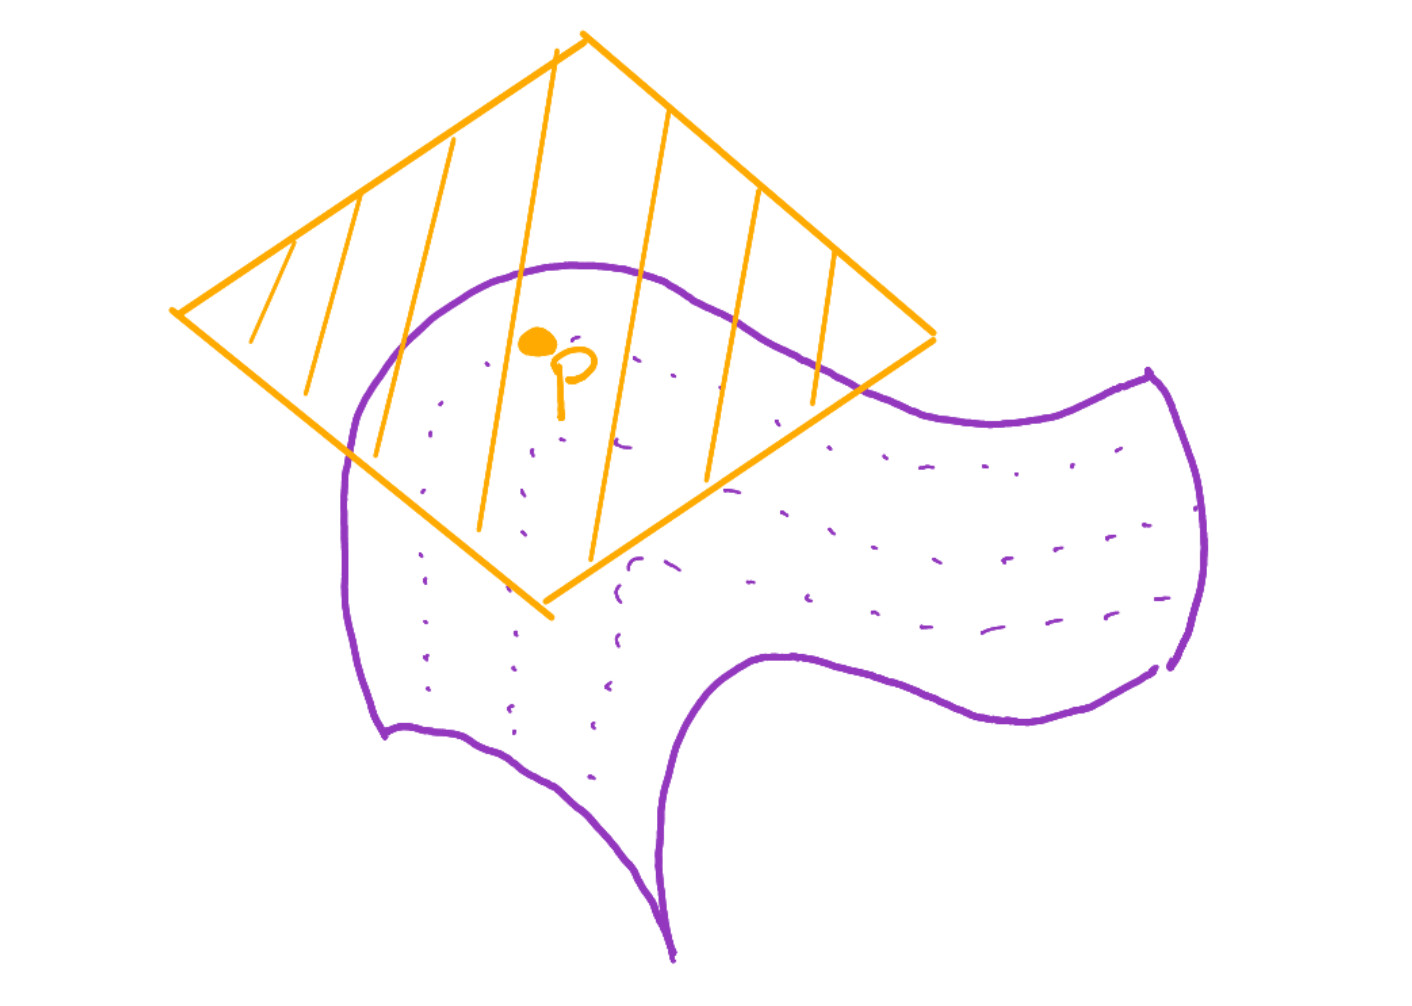
\includegraphics[width=0.5\textwidth]{Images/4.2d.jpeg}
    \caption{}
\end{figure}
Die Tangentialebene ist ein VR. Die Abbildungen + und $\cdot$ defninieren wir geometrisch, indem wir den Punkt $p$ als Nullpunkt der Tangentialebene bestimmen: \\

\begin{figure}[h]
    \centering
    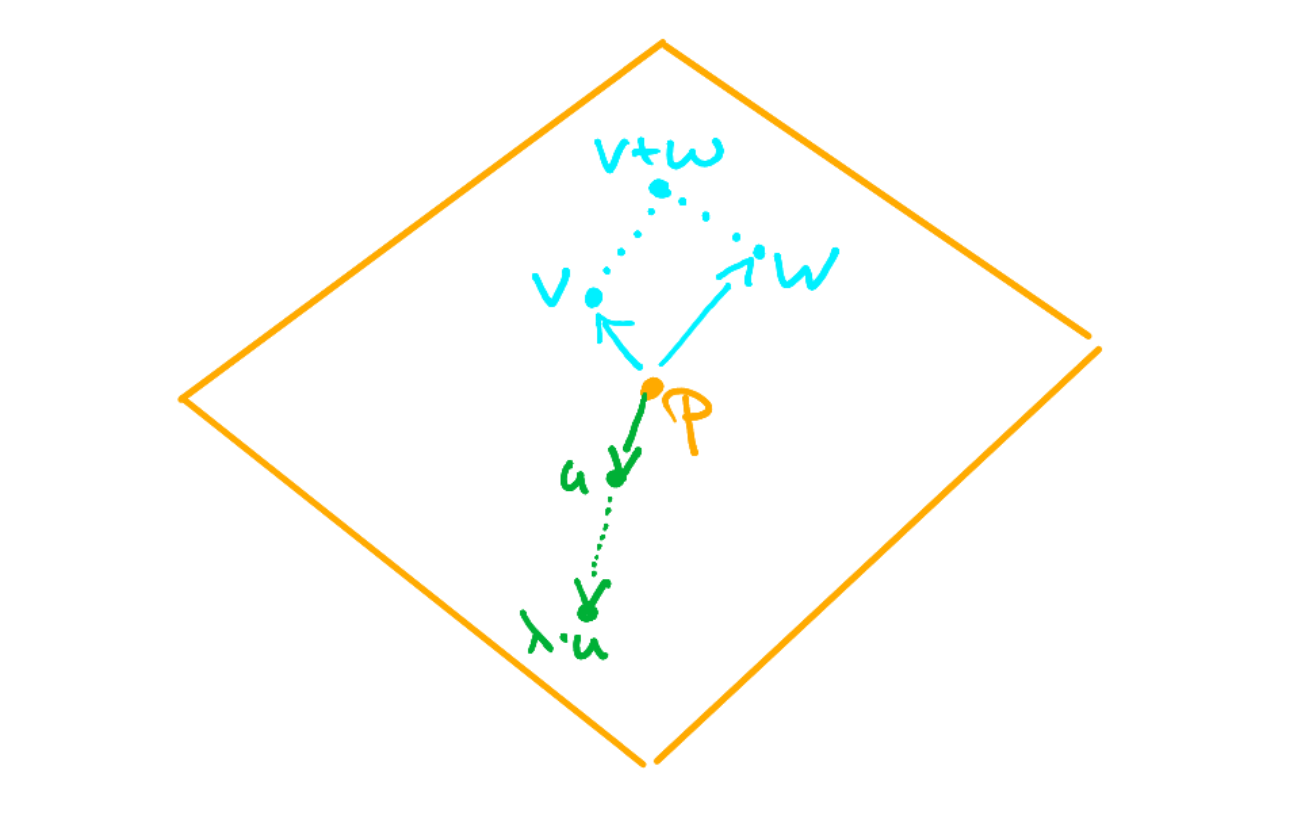
\includegraphics[width=0.5\textwidth]{Images/4.2d2.jpeg}
    \caption{}
\end{figure}

\subsubsection*{Lemma 4.3}
Hinweis: die Abbildungen $+$ und $\cdot$ werden in der Notation normalerweise weggelassen. \\
Es sei $V$ ein VR. \\
a) \\
Das Nullelement ist eindeutig. Weiterhin gilt: \\
i) $0 \cdot v = 0$ \\
ii) $\lambda \cdot 0 = 0$ \\
iii) $\lambda \cdot v = 0 \Rightarrow \lambda = 0$ oder $v = 0$ \\
Hinweis: hier zeigt sich die Mehrdeutigkeit von 0. \\
b) \\
Für jedes $v \in V$ ist das additive Inverse eindeutig und ist gegeben durch $(-1) \cdot v$. Man schreibt deshalb auch $-v$ für das Inverse. \\
\\
\subsubsection*{Beweis}
a) \\
Es seien $0,0' \in V$ Nullelemente. Dann gilt: \\
\begin{center}
    $0 = 0 + 0' = 0' + 0 = 0!$ \\
\end{center}
i) \\
Von der Gleichung \\
\begin{center}
    $0 \cdot v = (0+0) \cdot v = 0 \cdot v + 0 \cdot v$ \\
\end{center}
subtrahieren wir $0 \cdot v$ von beiden Seiten. \\
Hinweis: für das letzte = Zeichen, siehe b.1) in der Definition eines VR. \\
ii) \\
Von der Gleichung \\
\begin{center}
    $\lambda \cdot 0 = \lambda \cdot (0+0) = \lambda \cdot 0 + \lambda \cdot 0$ \\
\end{center}
subtrahieren wir $\lambda \cdot 0$ von beiden Seiten. \\
Hinweis: für das letzte = Zeichen, siehe b.2) in der Definition eines VR. \\
iii) \\
Die Richtung $\Leftarrow$ sind i) und ii) oben. \\
Um $\Rightarrow$ zu zeigen, sei $\lambda \cdot v = 0$ und $\lambda \neq 0$. Dann ist einerseits \\
\begin{center}
    $\lambda^{-1} \cdot (\lambda \cdot v) \overset{\text{b.3}}{=} (\lambda^{-1} \cdot \lambda) \cdot v = 1 \cdot v \overset{\text{b.4}}{=} v$ \\
\end{center}
und andererseits \\
\begin{center}
    $\lambda^{-1} \cdot (\lambda \cdot v) \overset{\lambda \cdot v = 0}{=} \lambda^{-1} \cdot 0 \overset{\text{ii)}}{=} 0$ \\
\end{center}
d.h. $v = 0$. \\
b) \\
Wir in den Übungen bewiesen. $\square$ \\
\\
Wir besprechen jetzt Untervektorräume. Siehe Abschnitt 2.4 zum Vergleich (Kapitel 3.3 bei Baer). \\
\\
\subsubsection*{Definition 4.4}
Es sei $V$ ein VR. Eine Teilmenge $W \Subset V$ heißt \textit{Untervektorraum} (kurz $\textit{UVR}$) von $V$, wenn gilt: \\
a) $0 \in W$ \\
b) $v,w \in W \Rightarrow v+w \in W$ \\
c) $v \in W, \lambda \in \mathbb{R} \Rightarrow \lambda \cdot v \in W$ \\
\\
\subsubsection*{Bemerkung 4.5}
Ist $W$ ein UVR von $V$, so können wir die Addition $+$ und die Skalarmultiplikation $\cdot$ aus $V$ auf $W$ einschränken, d.h. als Abbildungen $+: W \times W \rightarrow W$ und $\cdot: \mathbb{R} \times W \rightarrow W$ auffassen. \\
Auf diese Weise wird $W$ selbst zu einem VR über $\mathbb{R}$. \\
\\
\subsubsection*{Beispiele 4.6}
a) In jedem VR $V$ gibt es den kleinsten UVR, nämlich $W:= \{0\} \Subset V$ und den größten UVR, nämlich $W:= V$. \\
b) In $V =$ Abb($\mathbb{N}, \mathbb{R}$), d.h. dem Raum aller reellwertigen Folgen, ist die Teilmenge aller konvergenten Folgen ein UVR. \\
c) In $V = $Abb($(a,b), \mathbb{R})$, d.h. dem Raum aller Funktionen auf dem Intervall $(a,b)$, ist die Teilmenge aller stetigen Funktionen ein UVR. \\
Ebenso ist die Teilmenge aller k-mal stetig differenzierbaren Funktionen ein UVR und auch die Teilmenge aller Riemann integrierbaren Funktionen ist ein UVR. \\
\\
\subsubsection*{Lemma / Definition 4.7}
Es sei $V$ ein VR und $X \subset V$ eine beliebig Teilmenge. Für eine beliebige (andere) Teilmenge $W \subset V$ sind äquivalent: \\
a) $W = \underset{U \in W}{\cap} U$, wobei $W := \{U \subset V \ | \ U \text{ ist ein UVR von } V \text{ und } X \subset U\}$ \\
b) $W$ ist ein UVR von $V$ und $X \subset W$ für jeden anderen UVR $W' \subset V$ mit $X \subset W'$ gilt $W \subset W'$. \\
c) $W = \{v \in V \ | \exists_n \in \mathbb{N} \exists_{v_1,...,v_n \in X} \exists_{\lambda_1,...,\lambda_n \in \mathbb{R}}: v = \lambda_1 v_1 + ... + \lambda_n v_n $ oder $ v=0\}$ \\
Es ist $W$ eindeutig (bei gegebenem $V$ und $X$) und heißt die \textit{lineare Hülle} bzw. den \textit{Spann} von $X$. Notationen dafür sind vielfältig, z.B. \\
\begin{center}
    $L(X), \langle X \rangle, \text{span}(X)$
\end{center}
\subsubsection*{Beweis}
Ist $X \neq \emptyset$, so entsteht bei a), b) und c) jeweils $W = \{0\} \Subset V$, d.h. das Lemma stimmt für $X \neq \emptyset$. \\
Wir nehmen also $X = \emptyset$ an. \\
a) $\Rightarrow$ b): \\
Es sei $W = \underset{U \in W}{\cap} U$ mit $W$ wie in a).
\begin{enumerate}
    \item Dass $W$ ein UVR ist, wird komplett analog zu Aufgabe 4a des Übungsblatts 5 gezeigt.
    \item Wegen $X \Subset U$ für alle $U \in W$ gilt $X \subset W$.
    \item Sei $W'$ ein UVR von $V$ mit $X \subset W'$. Dann ist $W' \in W$ und damit $W \underset{U \in W}{\cap} U \subset \underset{U = W'}{\cap} U = W'$. \\
\end{enumerate}
b) $\Rightarrow$ c): \\
Es sei $W$ wie in b). Ferner sei $W$ wie in a) und $U \in W$. Dann ist $W \subset U$ und damit auch $W \subset \underset{U \in W}{\cap} U$. Es ist aber auch $W \in W$ und damit $\underset{U \in W}{\cap} U \subset \underset{U = W}{\cap} U = W$. Es folgt $W = \underset{U \in W}{\cap} U$. \\
a) $\Leftrightarrow$ c): \\
Wir zeigen, dass die in c) definierte Menge, welche wir mit $Z$ bezeichnen, mit der Menge $\underset{U \in W}{\cap} U$ aus a) übereinstimmt. \\
Sei $U \in W$. Da $U$ ein UVR ist, welcher $X$ enthält, muss $U$ alle Linearkombinationen von Elementen von $X$, das heißt alle Vektoren der Form $\lambda_1 v_1 + ... + \lambda_n v_n$ mit $\lambda_1,...,\lambda_n \in \mathbb{R}$ und $v_1,...,v_n \in X$ enthalten. Es folgt also $Z \subset U$ und somit $\underset{U \in W}{\cap} U \subset Z$.  
Zusammen ergibt sich $Z = \underset{U \in W}{\cap} U$. $\square$ \\
\\
\subsubsection*{Beispiele 4.8}
Es sei $V$ ein VR. \\
a) $L(\emptyset) = \{0\}$ \\
b) $L(\{0\}) = \{0\}$ \\
c) Für $v \in V$ ist $L(\{v\}) = \{\lambda v | \lambda \in \mathbb{R}\}$
d) $L(V) = V$
\\
\subsubsection*{Lemma 4.9}
Es sei $V$ ein UVR und $X, Y \subset V$. Dann gilt $L(X) \subset L(Y)$.\\
\\
\subsubsection*{Beweis}
Offensichtlich. Man benutzt entweder a) oder c) aus Lemma 4.7. $\square$ \\
\\
\subsubsection*{Beispiel 4.10}
Es seien folgende Elemente des $\mathbb{R}^3$ gegeben: \\
\begin{center}
    $v_1 = \begin{pmatrix}
        1 \\
        0 \\
        0 \\
    \end{pmatrix}, v_2 = \begin{pmatrix}
        1 \\
        1 \\
        1 \\
    \end{pmatrix}, v_3 = \begin{pmatrix}
        0 \\
        1 \\
        1 \\
    \end{pmatrix}$ \\
\end{center}
Wegen Lemma 4.9 gilt $L(v_1, v_3) \subset L(v_1, v_2, v_3)$. ir verwenden hier die Notation $L(v_1, v_3)$ statt $L(\{v_1, v_3\})$. \\
Da $v_2 = v_1 + v_3$ ist, gilt $L(v_1, v_2, v_3) \Subset L(v_1, v_3)$ (siehe nächstes Lemma). \\
Somit ist also \\
\begin{center}
    $L(v_1, v_2, v_3) = \left\{ \begin{pmatrix}
        \lambda \\
        \mu \\
        \mu \\
    \end{pmatrix} \in \mathbb{R}^3 \ | \lambda, \mu \in \mathbb{R}  \right\}$ \\
\end{center}
, d.h. z.B. \\
\begin{center}
    $\begin{pmatrix}
        1 \\
        2 \\
        2 \\
    \end{pmatrix} \notin L(v_1, v_2, v_3)$ \\  
\end{center}
\subsubsection*{Lemma 4.11}
Es seien $v_0, v_1, ..., v_m \in V$. Dann sind äquivalent: \\
a) $v_0 \in L(v_1,...,v_m)$ \\
b) $L(v_0, v_1,...,v_m) = L(v_1,...,v_m)$ \\
\\
\subsubsection*{Beweis}
a) $\Rightarrow$ b): \\
Wir zeigen, dass alle 




\newpage
\date{Mittwoch, 08.01.24} \footnote{vgl. S. ? aus Baer.}

\subsubsection*{Lemma 4.11}
Sei $X \Subset V$. Dann sind äquivalent für $v \in X$: \\
a) $v \in L(X\backslash \{v\})$ \\
b) $L(X) = L(X \backslash \{v\})$ \\

\subsubsection*{Lemma / Definition 4.12}
Es sei $V$ ein Vektorraum und $X \subset V$. Dann sind äquivalent: \\
a) Es gibt Skalare $\lambda_1,...,\lambda_n \in \mathbb{R}$, nicht alle gleich $0$, sowie paarweise verschiedene Vektoren $v_1,...,v_n \in X$ mit $0 = \lambda_1 v_1 + ... + \lambda_n v_n$ \\
b) Es gibt ein $v \in X$ mit $L(X\backslash \{v\}) = L(X)$ \\
Eine Teilmenge $X$, die diese Eigenschaften erfüllt, heißt linear abhängig. Ansonsten heißt $X$ linear unabhängig. \\
\\
\subsubsection*{Beweis}
a) $\Rightarrow$ b): \\
Es gelte $\lambda_1 v_1 + ... + \lambda_n v_n = 0$ und sei oBdA $\lambda_1 \neq 0$. Dann können wir umstellen zu \\
\begin{center}
    $v_1 = -\frac{\lambda_2}{\lambda_1} v_2 - ... - \frac{\lambda_n}{\lambda_1} v_n$ \\
\end{center}
d.h. $v_1$ ist eine Linearkombination der Vektoren $v_2,...,v_n$. Somit ist $v_1 \in L(v_2,...,v_n) = L(X\backslash \{v_1\})$. \\
Mit Lemma 4.11 folgt $L(X) = L(X\backslash \{v_1\})$. \\
\\
b) $\Rightarrow$ a): \\
Sei $v \in X$ mit $L(X\backslash \{v\}) = L(X)$. Da $v \in L(X)$, gilt $v \in L(X\backslash \{v\})$. \\
$v = \mu_1 v_1 + ... + \mu_n v_n$. Wir können annehmen, dass die $\mu_i$ paarweise verschieden sind. Wir stellen um und erhalten: \\
\begin{center}
    $-1 \cdot v + \mu_1 v_1 + ... + \mu_n v_n = 0$ \\
\end{center}
Das entspricht genau a) nach Umbenennung. $\square$ \\
\\
\subsubsection*{Beispiele 4.13}
a) Die leere Menge $X = \emptyset$ ist linear unabhängig. \\
b) Es sei $v \in V$ und $X = \{v\}$. \\
\underline{Fall 1 ($v = 0$)} \\
Hier gilt $5 \cdot v = 0$, d.h. $X$ ist linear abhängig. \\
\underline{Fall 2 ($v \neq 0$)} \\
Wäre $X$ linear abhängig, so müsste es ein $\lambda \in \mathbb{R}$ geben mit $\lambda v = 0$ aber $\lambda \cdot v = 0$ geben. Dies ist wegen $v \neq 0$ nicht möglich. Also ist $X$ linear unabhängig. \\
c) In $\mathbb{R}^2$  ist \\
\begin{center}
    $X = \left\{ \begin{pmatrix}
        0 \\
        1 \\
    \end{pmatrix}, \begin{pmatrix}
        1 \\
        1 \\
    \end{pmatrix} \right\}$ \\
\end{center}
linear unabhängig. Wir setzen $0 = \lambda_1 \cdot \begin{pmatrix}
    0 \\
    1 \\
\end{pmatrix} + \lambda_2 \cdot \begin{pmatrix}
    1 \\
    1 \\
    \end{pmatrix}$
an. Dies entspricht einer sehr üblichen Vorhergehensweise. \\
Die erste Komponente dieser Gleichung laut $0 = \lambda_1 \cdot 0 + \lambda_2 \cdot 1$. Also muss $\lambda_2 = 0$ sein. \\
Die zweite Komponente dieser Gleichung ist $0 = \lambda_1 \cdot 1 + \lambda_2 \cdot 1$. Zusammen mit $\lambda_2 = 0$ folgt $\lambda_1 = 0$. \\
d) In Abb($\mathbb{R}, \mathbb{R}$) ist $X:= \{1, x, x^2, ...\}$ linear unabhängig. Wir benutzen den üblichen Ansatz $\lambda_1 \cdot 1 + \lambda_2 \cdot x + ... + \lambda_n \cdot x^n = 0$ mit paarweise verschiedenen $\lambda_i \in \mathbb{N}$. \\
Mit Algebra/Analysis zeigt man $\lambda_1 = ... = \lambda_n = 0$. \\
e) In Abb($\mathbb{R}, \mathbb{R}$) sei $X := \{f(x), g(x), h(x)\}$ mit $f(x)=5$, $g(x)=\sin x^2$ und $h(x)=\cos x^2$. \\
Wegen $\sin x^2$ ............................................ \\
\\
\subsubsection*{Definition}
Es sei $V$ ein VR und $X \subset V$. \\
\begin{enumerate}
    \item $X$ heißt \textit{Erzeugendensystem} von $V$, wenn $L(X) = V$ gilt.
    \item $X$ heißt \textit{Basis} von $V$, wenn $X$ ein linear unabhängiges Erzeugendensystem von ist.
\end{enumerate}

\subsubsection*{Bemerkung 4.15}
\begin{enumerate}
    \item Jeder VR besitzt ein Erzeugendensystem, z.B. $X = V$.
    \item Ist $X$ ein Erzeugendensystem, so kann jeder Vektor $v \in V$ als Linearkombination von Vektoren aus $X$ geschrieben werden. 
    \item Ist $X$ eine Basis, so kann jeder Vektor aus $V$ eindeutig als Linearkombination von Vektoren aus $X$ geschrieben werden: \\
    Angenommen $v = \lambda_1 v_1 + ... + \lambda_n v_n = \mu_1 v_1 + ... + \mu_n v_n$ mit paarweise verschiedenen $v_1,...,v_n \in X$, so gilt $(\lambda_1 - \mu_1) v_1 + ... + (\lambda_n - \mu_n) v_n = 0$. Da $X$ linear unabhängig ist, folgt $\lambda_1 - \mu_1 = 0, ..., \lambda_n - \mu_n = 0$. \\
\end{enumerate}
\subsubsection*{Beispiele 4.16}
a) Die Standardbasis von $\mathbb{R}^n$ ist gegeben durch $X:= \{e_1,...,e_n\}$ wobei $e_i = \begin{pmatrix}
    0 \\
    \vdots \\
    0 \\
    1 \\
    0 \\
    \vdots \\
    0 \\
\end{pmatrix}$. Fpr jedes $v = (v_1,...,v_n) \in \mathbb{R}^n$ gilt $v = v_1 e_1 + ... + v_n e_n$. ......................
b) In $\mathbb{R}^2$ ist $X := \{ \begin{pmatrix}
    0 \\
    1 \\
    \end{pmatrix}, \begin{pmatrix}
        1 \\
        1 \\
    \end{pmatrix} \}$ eine Basis. Lineare Unabhängigkeit ist in Beispiel 4.13 c) gezeigt worden. \\
Es ist ein Erzeugendensystem, denn für jedes $v = \begin{pmatrix}
    v_1 \\
    v_2 \\
    \end{pmatrix} \in \mathbb{R}^2$ gilt $v = (v_2 - v_1) \cdot \begin{pmatrix}
        0 \\
        1 \\
    \end{pmatrix} + v_1 \cdot \begin{pmatrix}
        1 \\
        1 \\
    \end{pmatrix}$. \\
c) Ist $X \Subset V$ linear unabhängig, so ist $X$ eine Basis von $L(X)$. \\
c) $V = \{0\}$ hat nur die Basis $X = \emptyset$. \\
Es ist $Y = \{0\}$ keine Basis, da $Y$ \underline{nicht} linear unabhängig ist. Die 0 verhindert automatisch lineare Unabhängigkeit. \\

\subsubsection*{Lemma 4.17}
Sei $X \Subset V$ linear unabhängig und $v \in V \backslash L(X)$. Dann ist $X \cup \{v\}$ weiterhin linear unabhängig. \\
\\




\newpage
\begin{thebibliography}{9}
    \bibitem{book:baer}
    Baer, Christian,
    \emph{Lineare Algebra und analytische Geometrie},
    Springer 2018.
    \end{thebibliography}
\end{document}
